\documentclass[11pt]{report}
\usepackage{titlesec}
\titleformat{\chapter}
{\normalfont\LARGE\bfseries}{\thechapter}{1em}{}
\titlespacing*{\chapter}{0pt}{3.5ex plus 1ex minus .2ex}{2.3ex plus .2ex}

\usepackage[margin=1.2in]{geometry}
\usepackage[toc,page]{appendix}
\usepackage{graphicx}
\usepackage{lipsum}
\usepackage{caption}
\usepackage[utf8]{inputenc}
\usepackage[italian]{babel}
\usepackage{indentfirst}
\usepackage{verbatim}
\usepackage{colorprofiles}
\usepackage{listings}   %<- per inserire il codice
\usepackage{float}
\usepackage{subcaption}
\usepackage{amsmath}
\usepackage{amsfonts}
\usepackage{booktabs}
\usepackage{xcolor}
\usepackage{textcomp}
\usepackage{gensymb}
\usepackage[hidelinks]{hyperref}

%%%%%%%%%%%%%%%%%%%%%%%%%%%%%%%%%%%%%%%%%%%%%%%%%%%%%%%%%%%%%%%%%%%%
\definecolor{custom_green}{rgb}{0,0.6,0}
\definecolor{codegray}{rgb}{0.5,0.5,0.5}
\definecolor{custom_blue}{rgb}{0.05,0.05,0.97}
\definecolor{custom_purple}{rgb}{0.58,0.00,0.82}
\definecolor{custom_orange}{rgb}{0.94,0.59,0.09}


\lstdefinestyle{base}{
	language=C,
	backgroundcolor=\color{white},  
	basicstyle=\footnotesize\ttfamily\color{black},   
	breakatwhitespace=false,       
	breaklines=true,               
	columns=fullflexible,
	captionpos=b,                   
	commentstyle=\color{custom_green},   
	inputencoding=utf8,
	extendedchars=true,
	keepspaces=true,
	literate={à}{{\`a}}1 {è}{{\`e}}1 {é}{{\'e}}1 {ì}{{\`i}}1 {ò}{{\`o}}1 {ù}{{\`u}}1,
	escapeinside={\%*}{*)},
	keywordstyle=\color{custom_purple},
	identifierstyle=\color{custom_blue},
	stringstyle=\color{custom_orange},      
	numbers=left,                 
	numbersep=5pt,                  
	numberstyle=\tiny\color{codegray}, 
	rulecolor=\color{black},        
	showspaces=false,               
	showstringspaces=false,        
	showtabs=false,                
	stepnumber=1,                   
	tabsize=4,                     
}

\lstset{style=base}


%%%%%%%%%%%%%%%%%%%%%%%%%%%%%%%%%%%%%%%%%%%%%%%%%%%%%%%%%%%%%%%%%%%%




\begin{document}
	\captionsetup[figure]{margin=1.5cm,font=small,labelfont={bf},name={Figure},labelsep=colon,textfont={it}}
	\captionsetup[table]{margin=1.5cm,font=small,labelfont={bf},name={Table},labelsep=colon,textfont={it}}
	
	
	\begin{titlepage}
		\begin{center}
		\
			\LARGE {\scshape{Università Politecnica delle Marche}}\\[0.5cm]
			\LARGE {\scshape{Ingegneria Informatica e dell'Automazione}}\\[0.7cm]
			\linespread{1}
			\huge {\bfseries Ducted Fan }\\[1cm]
			\linespread{1}
			
\includegraphics[width=5cm]{figures/00_frontespizio/logo_univpm.jpg}\\[0.5cm]
			\linespread{1.2}
			\Large Corso di\\
			\Large {\scshape{Laboratorio di Automazione}} \\[0.3cm]
			\Large {Anno accademico 2025-2026 \\[0.8cm]}
			{\Large Studenti:}
			\hfill {\Large Professore:}\\
			\begin{minipage}[t]{0.48\textwidth}
				\raggedright
				{\Large Mencarelli Matteo}\\
				{\Large Secci Bianca}\\
				{\Large Tagliatesta Diego}
			\end{minipage}
			\hfill
			\begin{minipage}[t]{0.48\textwidth}
				\raggedleft
				{\Large Andrea Bonci}\\[0.4cm]
				{\Large Dottorando:}\\
				{\Large Alessandro Di Biase}
			\end{minipage}\\[1cm]
			{
				
\includegraphics[width=2cm]{figures/00_frontespizio/logo_dipartimento_dii.png}\\[0.3cm]
				\large Dipartimento di Ingegneria dell'Informazione\\[0.3cm]
			}
		\end{center}
	\end{titlepage}
	
	\pagenumbering{arabic}
	\tableofcontents
	\addcontentsline{toc}{chapter}{Introduzione}
	\newpage
	
	\pagestyle{plain}
	
	\section*{Introduzione}
	Spiegazione dettagliata del task assegnato al gruppo (cosa avete fatto e su quale sistema).
	Se per lo svolgimento del task è stato necessario interagire con altri gruppi che hanno lavorato sullo stesso sistema, presentare anche brevemente i task svolti dagli altri gruppi e spiegare la loro interconnessione.
	Se si è invece optato per far confluire il lavoro di più gruppi in un'unica relazione, va spiegato qual era il task iniziale dei singoli gruppi e poi come è avvenuta l'integrazione.
	In sintesi, l'introduzione deve permettere al lettore di capire subito su cosa avete lavorato.
	Al termine dell'introduzione inserite anche una breve descrizione per capitoli del contenuto della restante parte della relazione (es. nel Capitolo \ref{Hardware} viene descritto...).
	
	Nel seguito la struttura in capitoli di massima per ogni relazione, da adattare qualora necessario.
	\textcolor{red}{NOTA: La relazione va pensata e scritta nell'ottica di dare a chi verrà dopo di voi un documento utile per capire a che punto è arrivata l'attività svolta dal vostro gruppo e per metterli in condizione di portare avanti il vostro lavoro. Di conseguenza dovete essere chiari e diretti, riportando solo le informazioni necessarie e evidenziando in modo critico cosa effettivamente funziona correttamente e cosa va migliorato}
	
	\newpage
	\chapter{Sistema}
	Nel presente capitolo viene descritta la struttura meccanica del \textit{Double Propeller Ducted-Fan (DPDF)} e viene introdotto l'obiettivo di controllo adottato nel progetto.
	
	\section{Double Propeller Ducted-Fan. Struttura}
	Il \textit{DPDF} presenta una struttura cilindrica cava di \textbf{220 [mm]} di altezza e con un diametro esterno pari a \textbf{235 [mm]}. Il diametro interno, pari a \textbf{230 [mm]}, contiene le componenti necessarie al volo stabile dell'\textbf{UAV}.

	La configurazione con montaggio interno delle componenti responsabili del moto rappresenta l'elemento distintivo rispetto alle architetture di droni convenzionali. Tale configurazione risulta vantaggiosa per qualsiasi forma di interazione di contatto, sia con l'operatore umano sia con oggetti esterni, in quanto le eliche non sono esposte ma risultano integrate e protette dalla stessa struttura portante del drone.

	Proseguendo con la descrizione della struttura interna del \textit{DPDF}, nella parte superiore sono posizionati due motori disposti in configurazione controrotante. L'implementazione di tale assetto garantisce la generazione di spinte verticali senza che il drone ruoti su se stesso attorno all'asse Z, passante per il centro della struttura cilindrica. Le eliche, infatti, generano momenti torcenti in direzione opposta e, bilanciandosi, restituiscono un momento risultante nullo per il velivolo.

	Inoltre, l'adozione di due motori si è resa necessaria in quanto un singolo attuatore non sarebbe stato in grado di generare una spinta sufficiente a garantire la portanza richiesta dal sistema nelle condizioni operative previste. I motori sono ancorati a una struttura a croce usata sia come base sia come rinforzo per le sollecitazioni che il \textit{DPDF} può subire. Tale struttura è stata progettata con una geometria e una finitura superficiale tali da minimizzare l'insorgenza di turbolenze aerodinamiche potenzialmente destabilizzanti per il volo del drone.
	\begin{figure}[H]
		\centering
		\begin{subfigure}[b]{0.48\textwidth}
			\centering
			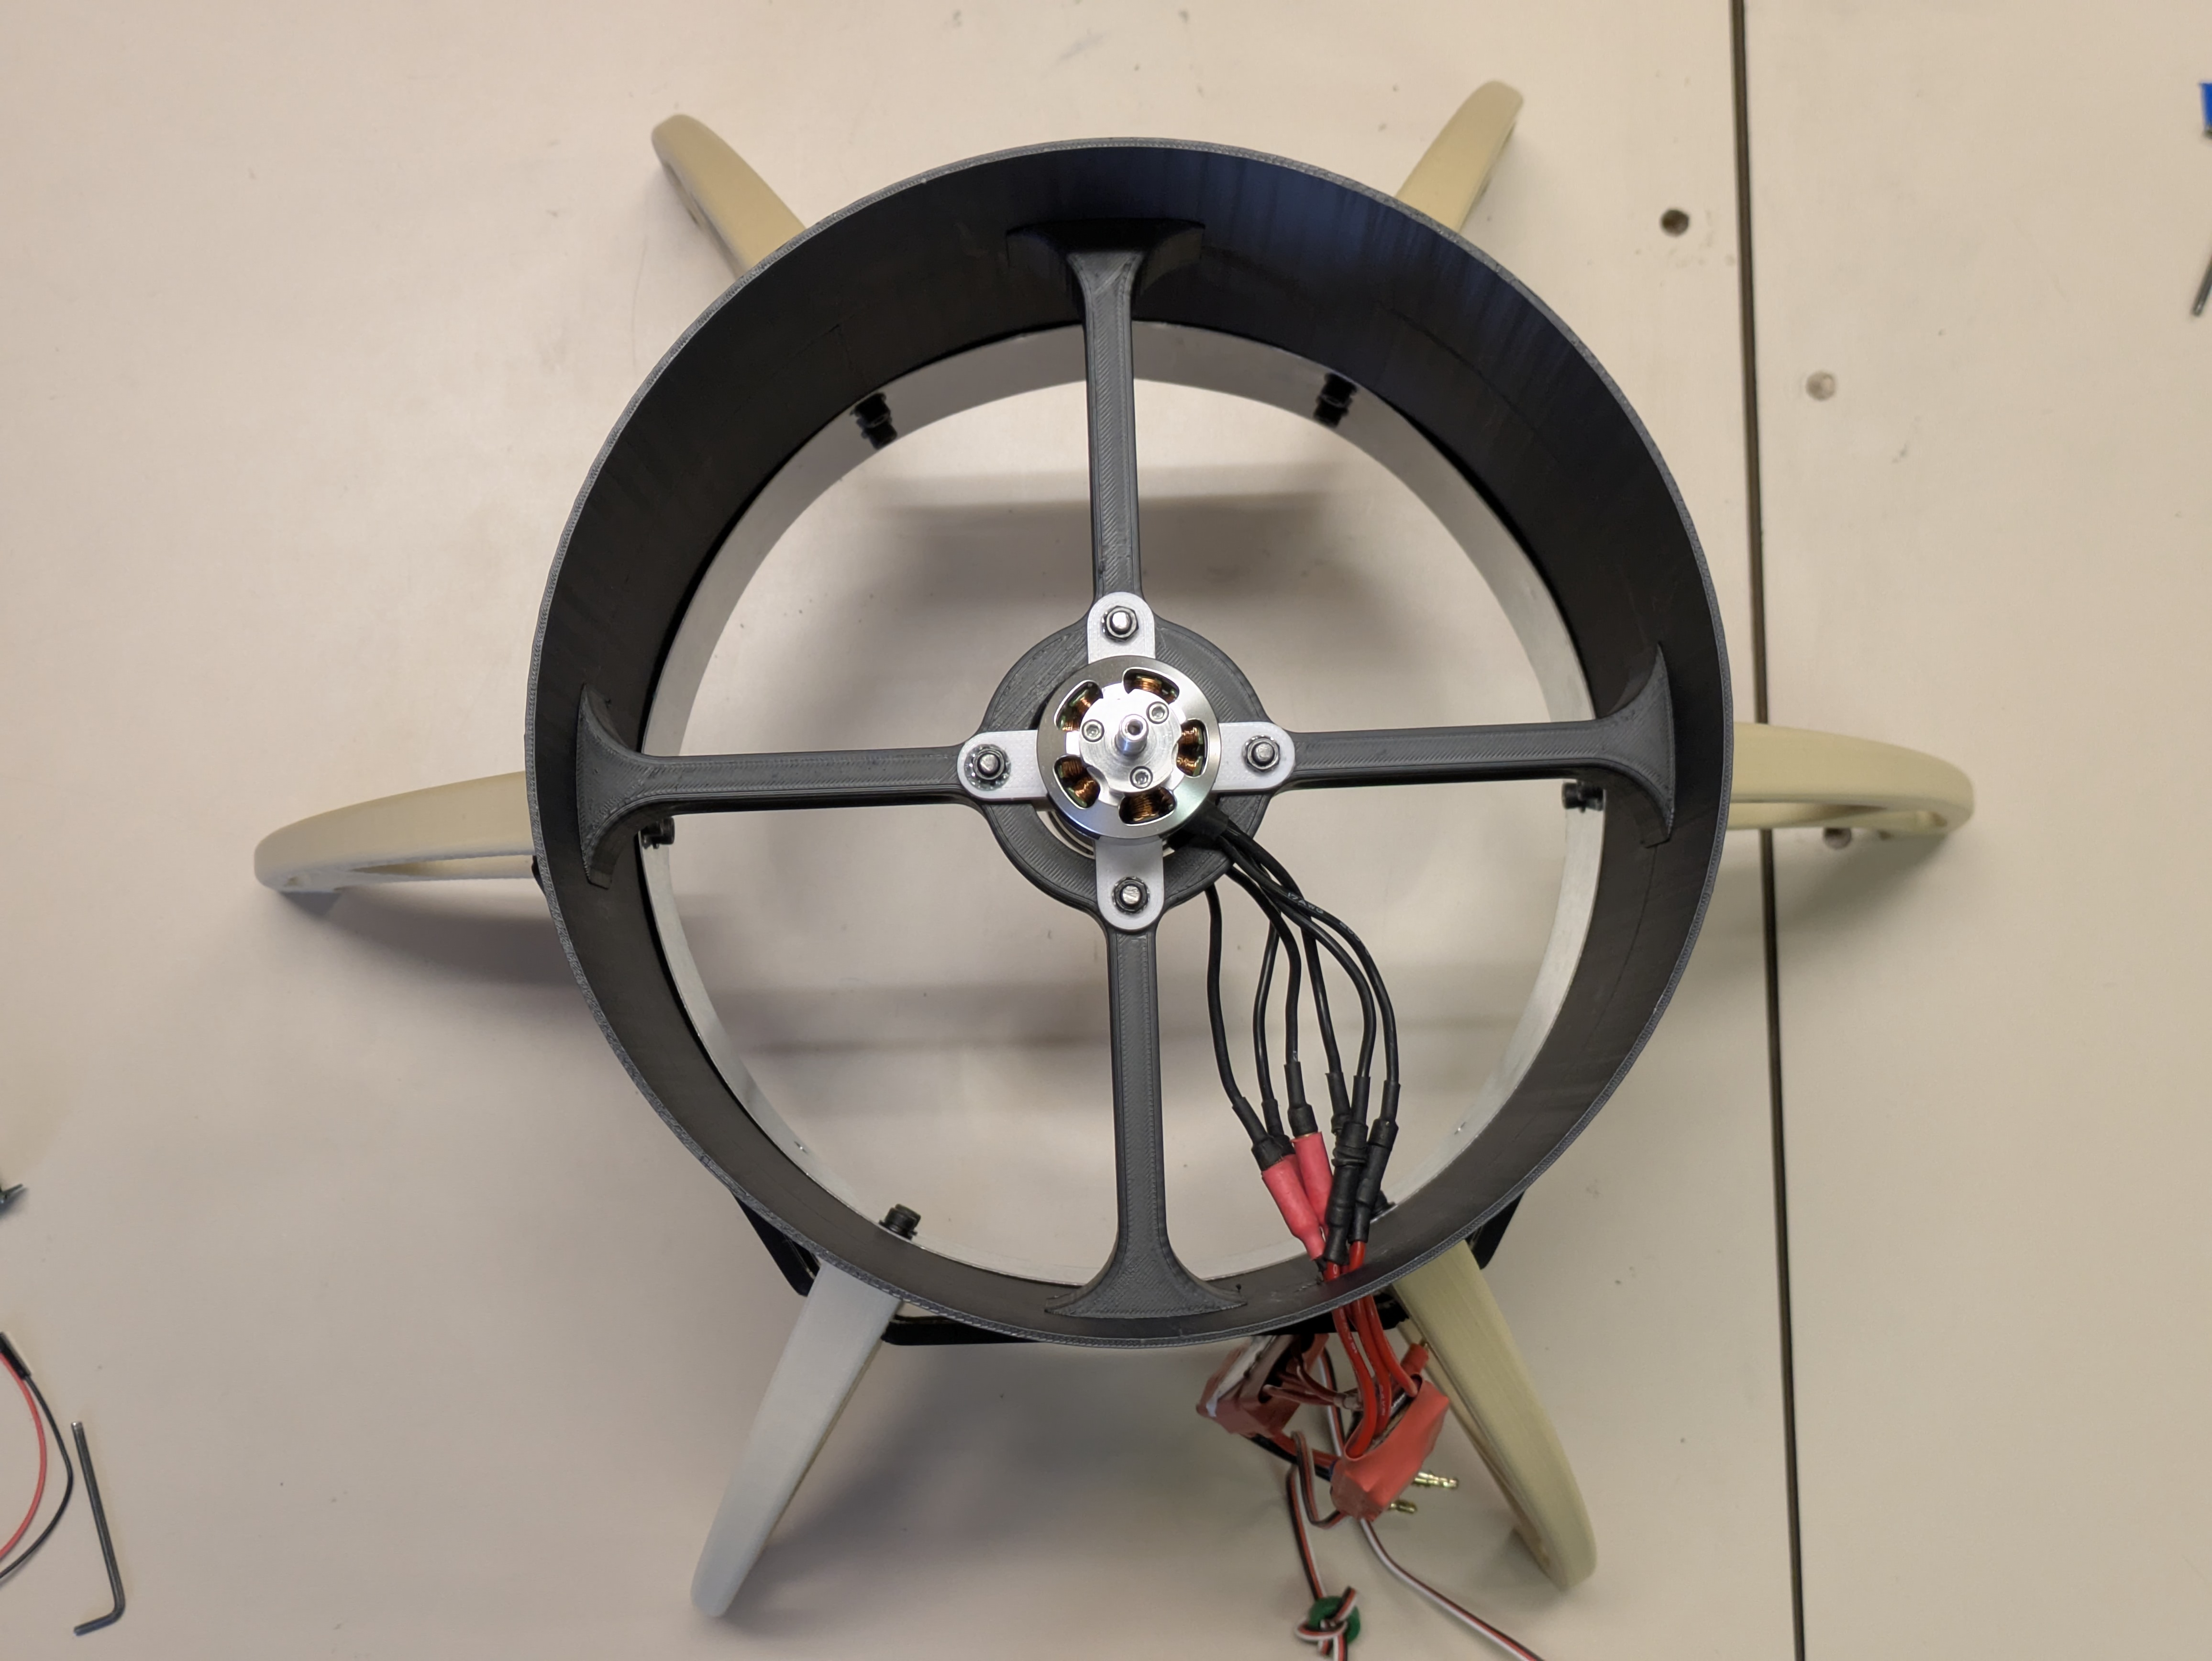
\includegraphics[height=4.5cm,keepaspectratio]{figures/01_sistema/struttura_ducted_fan_1.jpg}
			\caption{Struttura di sostegno dei motori}
		\end{subfigure}
		\hfill
		\begin{subfigure}[b]{0.48\textwidth}
			\centering
			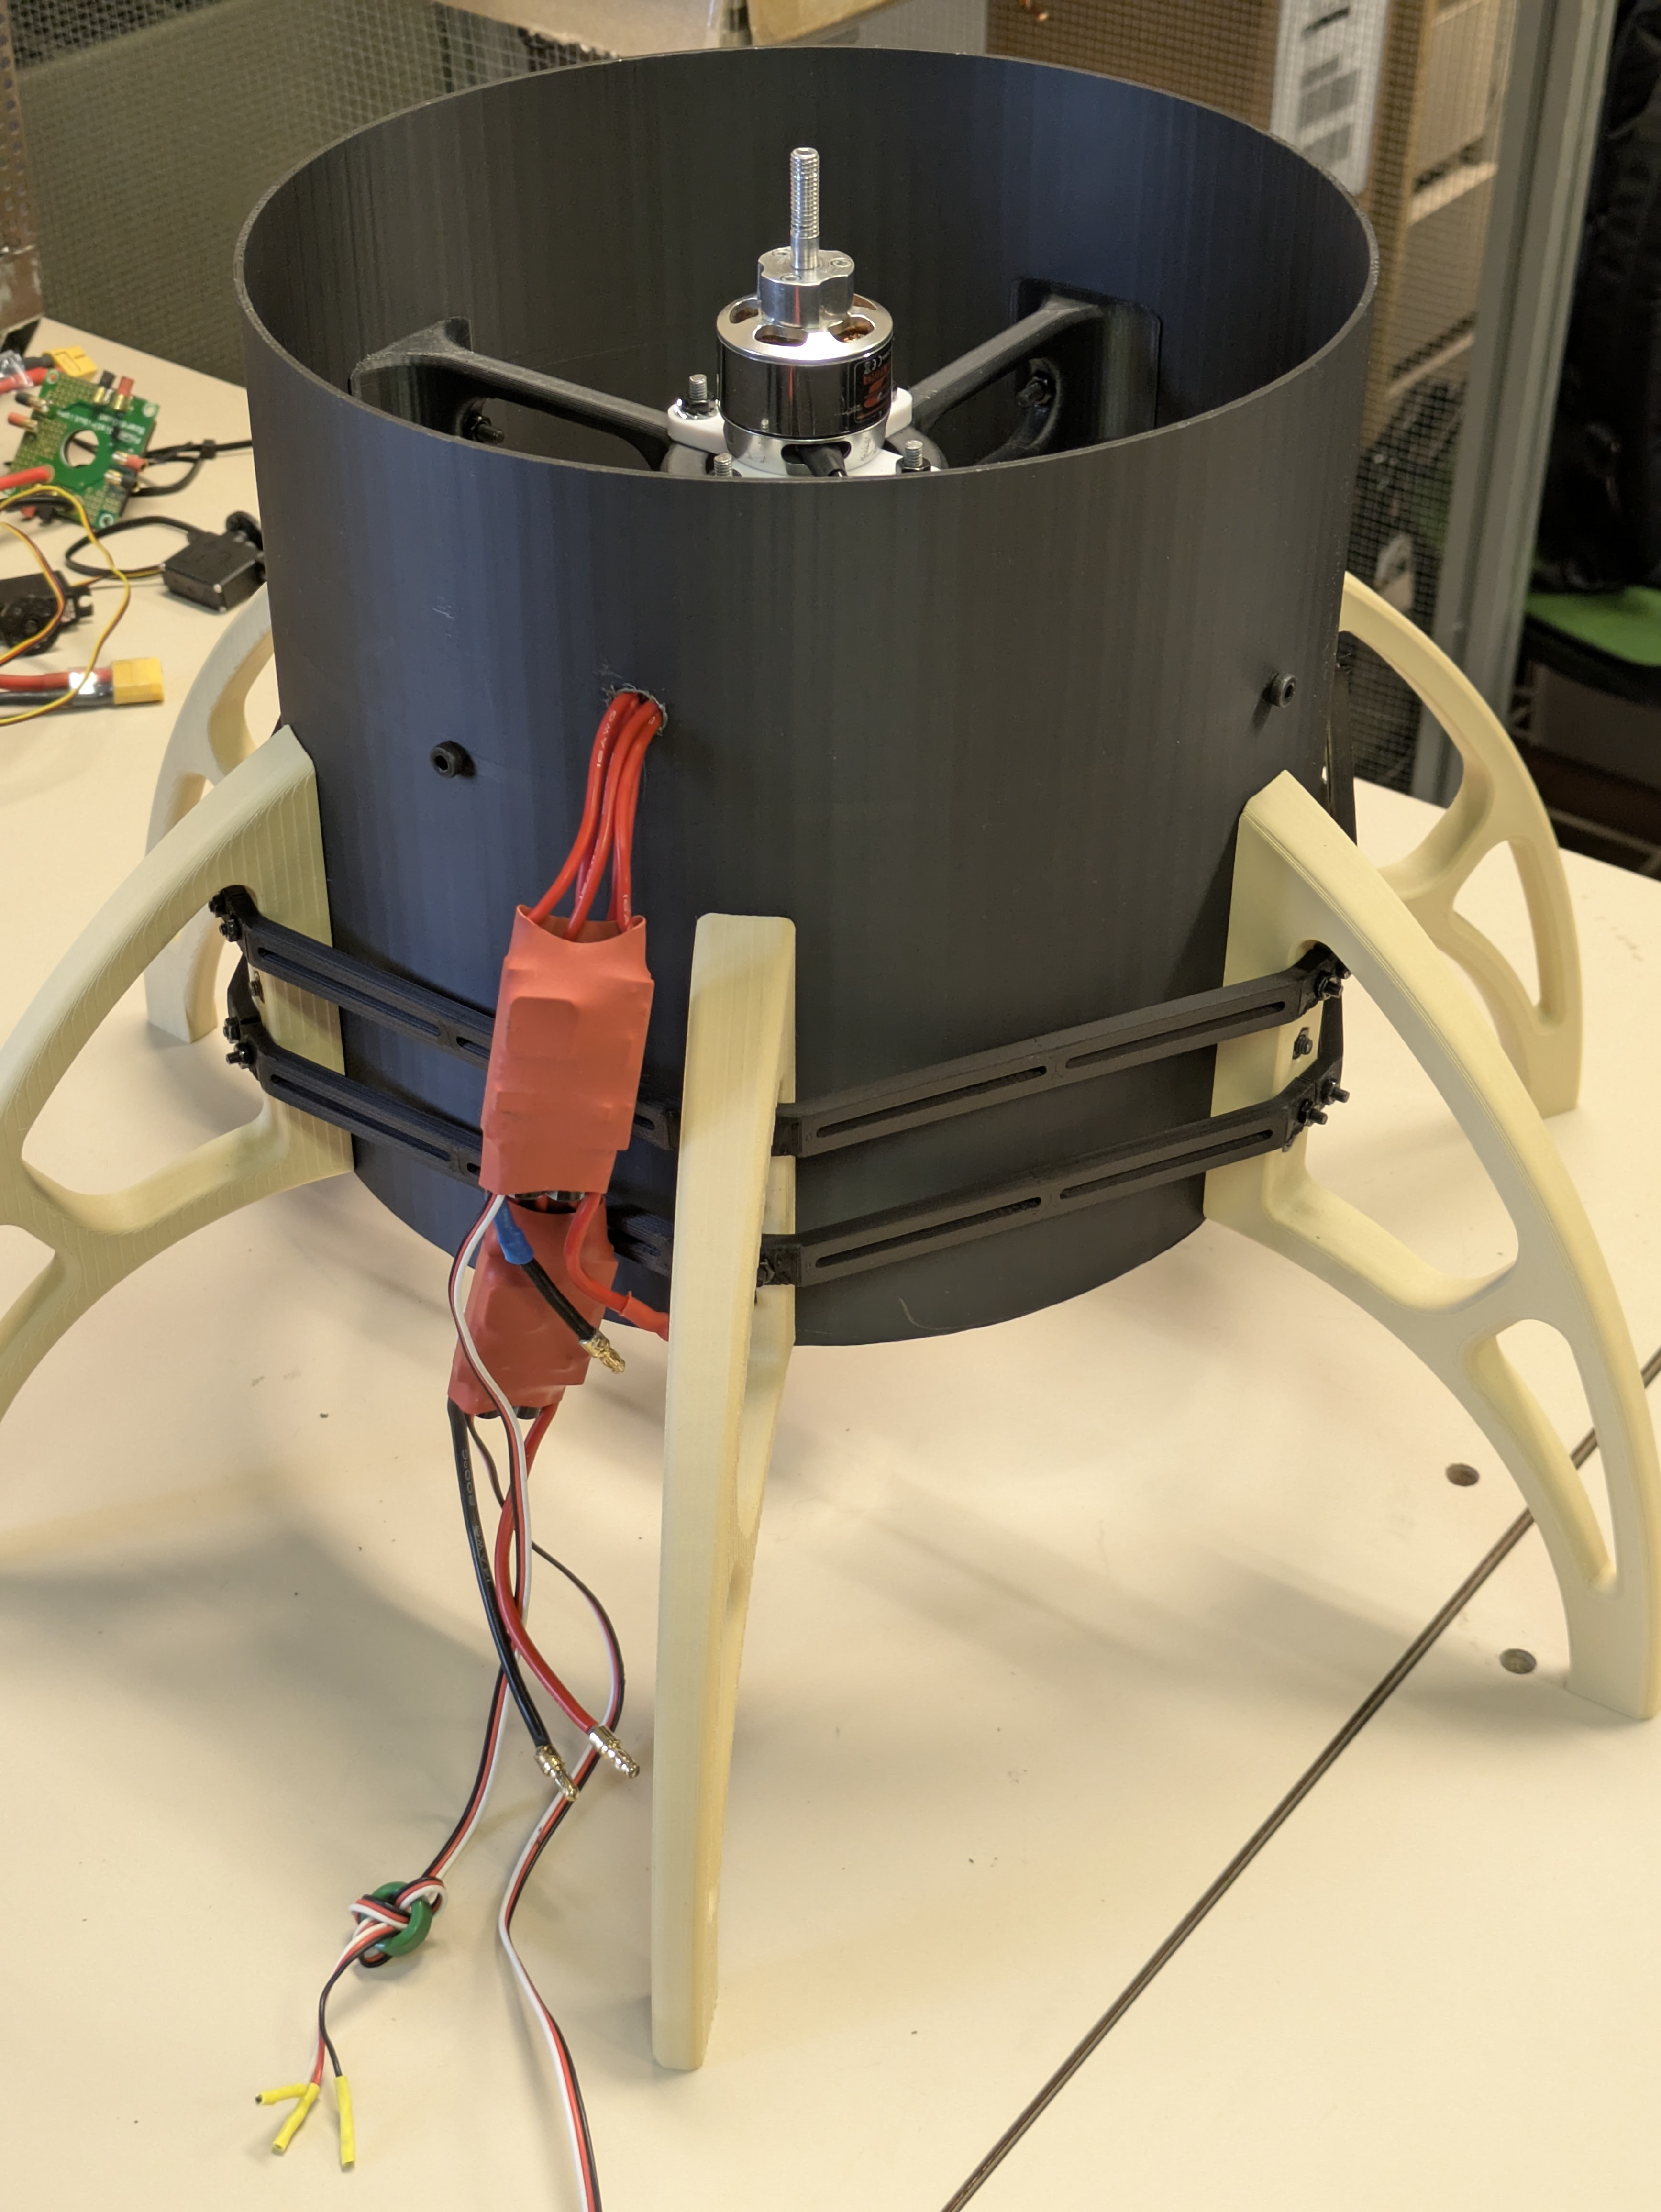
\includegraphics[height=4.5cm,keepaspectratio]{figures/01_sistema/struttura_ducted_fan_2.jpg}
			\caption{Vista frontale}
		\end{subfigure}
		\caption{\textcolor{black}{Struttura del ducted fan}}
		\label{fig:struttura_ducted_fan}
	\end{figure}
	Il disegno strutturale rende il \textit{DPDF} suscettibile a rotazioni indesiderate sul piano definito dagli assi X e Y. Tali perturbazioni possono compromettere la stabilità del sistema, determinando una completa perdita di controllo del mezzo.\\
	Al fine di limitare tali perturbazioni, la parte inferiore del \textit{DPDF} integra due \textbf{flap}: uno dedicato al controllo dell'assetto lungo l'asse delle ascisse e uno lungo l'asse delle ordinate.\\
	I \textit{flap}, interagendo con il getto d'aria generato dai motori, operano come superfici aerodinamiche di controllo dedicate alla compensazione dei disturbi di \textit{roll} e \textit{pitch}. L'intervento di regolazione si basa sulla modifica della direzione e della velocità del flusso d'aria spinto verso il basso. Il \textit{flap}, ruotando di un piccolo angolo, genera una deviazione del getto che lo investe. Tale deviazione produce una variazione della distribuzione di pressione tra il lato esposto al flusso (lato di pressione) e il lato opposto (lato di depressione). La differenza di pressione genera una forza aerodinamica risultante che produce un momento correttivo sull'assetto del velivolo. In prima approssimazione, la forza può essere considerata perpendicolare alla superficie del \textit{flap}. La direzione e il verso della forza devono essere tali da contrastare il momento perturbativo.\\
	Entrambi i \textit{flap} sono collegati, a un'estremità, al servomotore che ne gestisce il movimento, mentre all'altra sono inseriti in un apposito modulo strutturale che, oltre a fissare ciascun sensore del sistema, lo mantiene parallelo al terreno. I \textit{flap} sono posizionati in modo tale da risultare perpendicolari tra loro.\\
	Lungo la superficie esterna del cilindro sono state posizionate le componenti hardware necessarie al perseguimento degli scopi progettuali. La posizione di tali componenti è stata oggetto di studio al fine di ottenere un preciso bilanciamento del sistema. Gli elementi hardware utilizzati verranno approfonditi nel Capitolo 2.\\
	Inoltre, sulla superficie esterna sono montati sei piedi, posizionati in corrispondenza dei vertici dell'esagono in cui è inscritta la circonferenza del \textit{DPDF}. Tale configurazione permette di ottenere un'ottima distribuzione dei pesi. I piedi sono agganciati alla struttura mediante due bulloni opportunamente posizionati, il cui dado di fissaggio si trova all'esterno, lasciando così la testa all'interno. Tale impostazione permette di evitare l'allentamento del dado di fissaggio causato dal flusso d'aria incidente generato dai motori.\\
	L'intera struttura cilindrica, i \textit{flap}, i piedi di appoggio e i supporti di sostegno di tutte le componenti hardware e dei motori sono stati realizzati tramite \textbf{stampa 3D}, utilizzando \textbf{PVC} come materiale principale. Tutte le componenti sono state stampate separatamente e successivamente assemblate e fissate tra loro al fine di costruire la struttura completa del sistema.

	\begin{figure}[!htbp]
		\centering
		\begin{subfigure}[t]{0.9\textwidth}
			\centering
			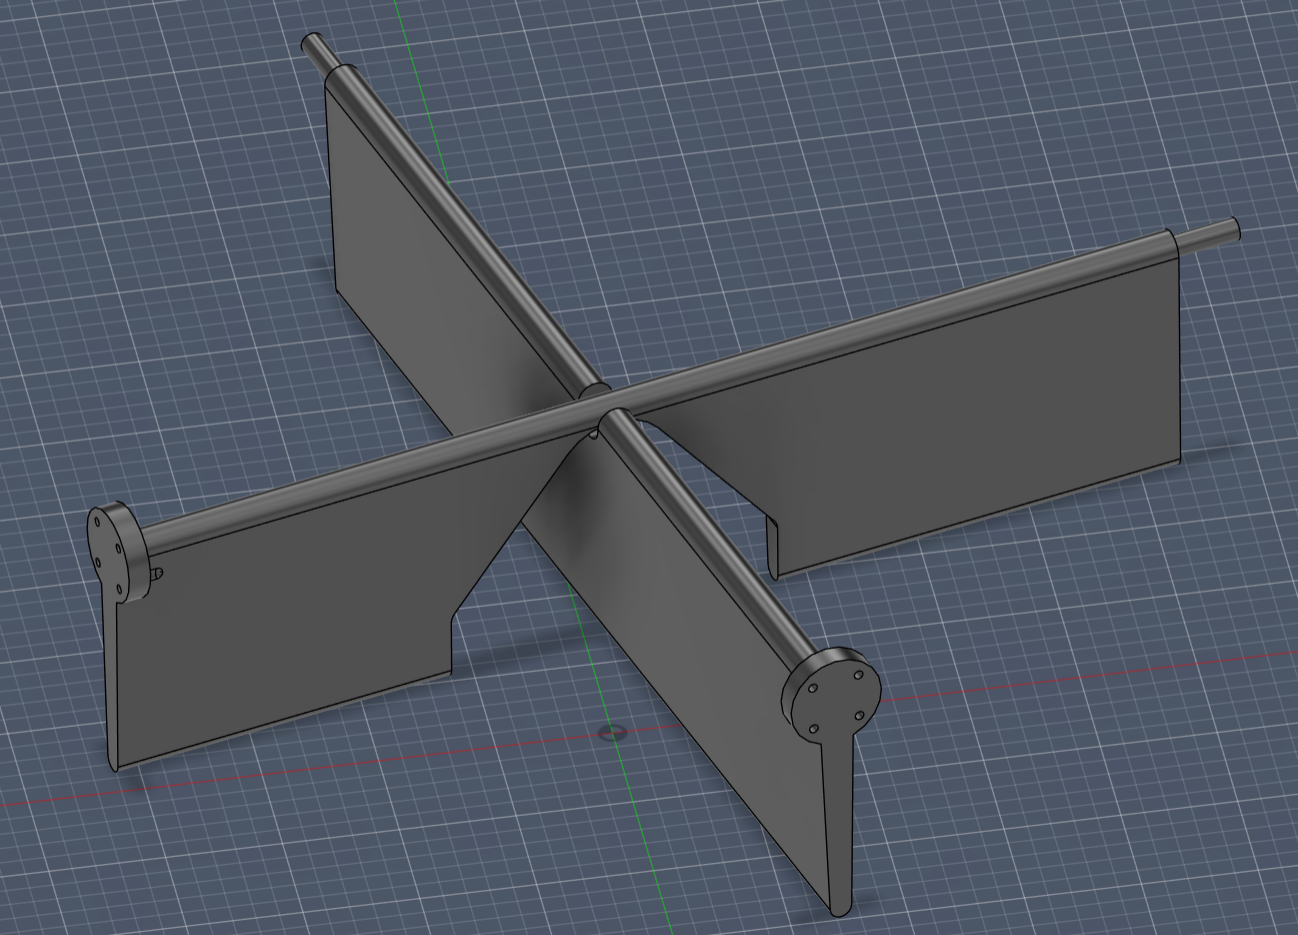
\includegraphics[height=5.4cm,keepaspectratio]{figures/01_sistema/image_fusion_1.png}
			\caption{Render flap}
		\end{subfigure}
		
		\vspace{0.5cm}
		
		\begin{subfigure}[t]{0.9\textwidth}
			\centering
			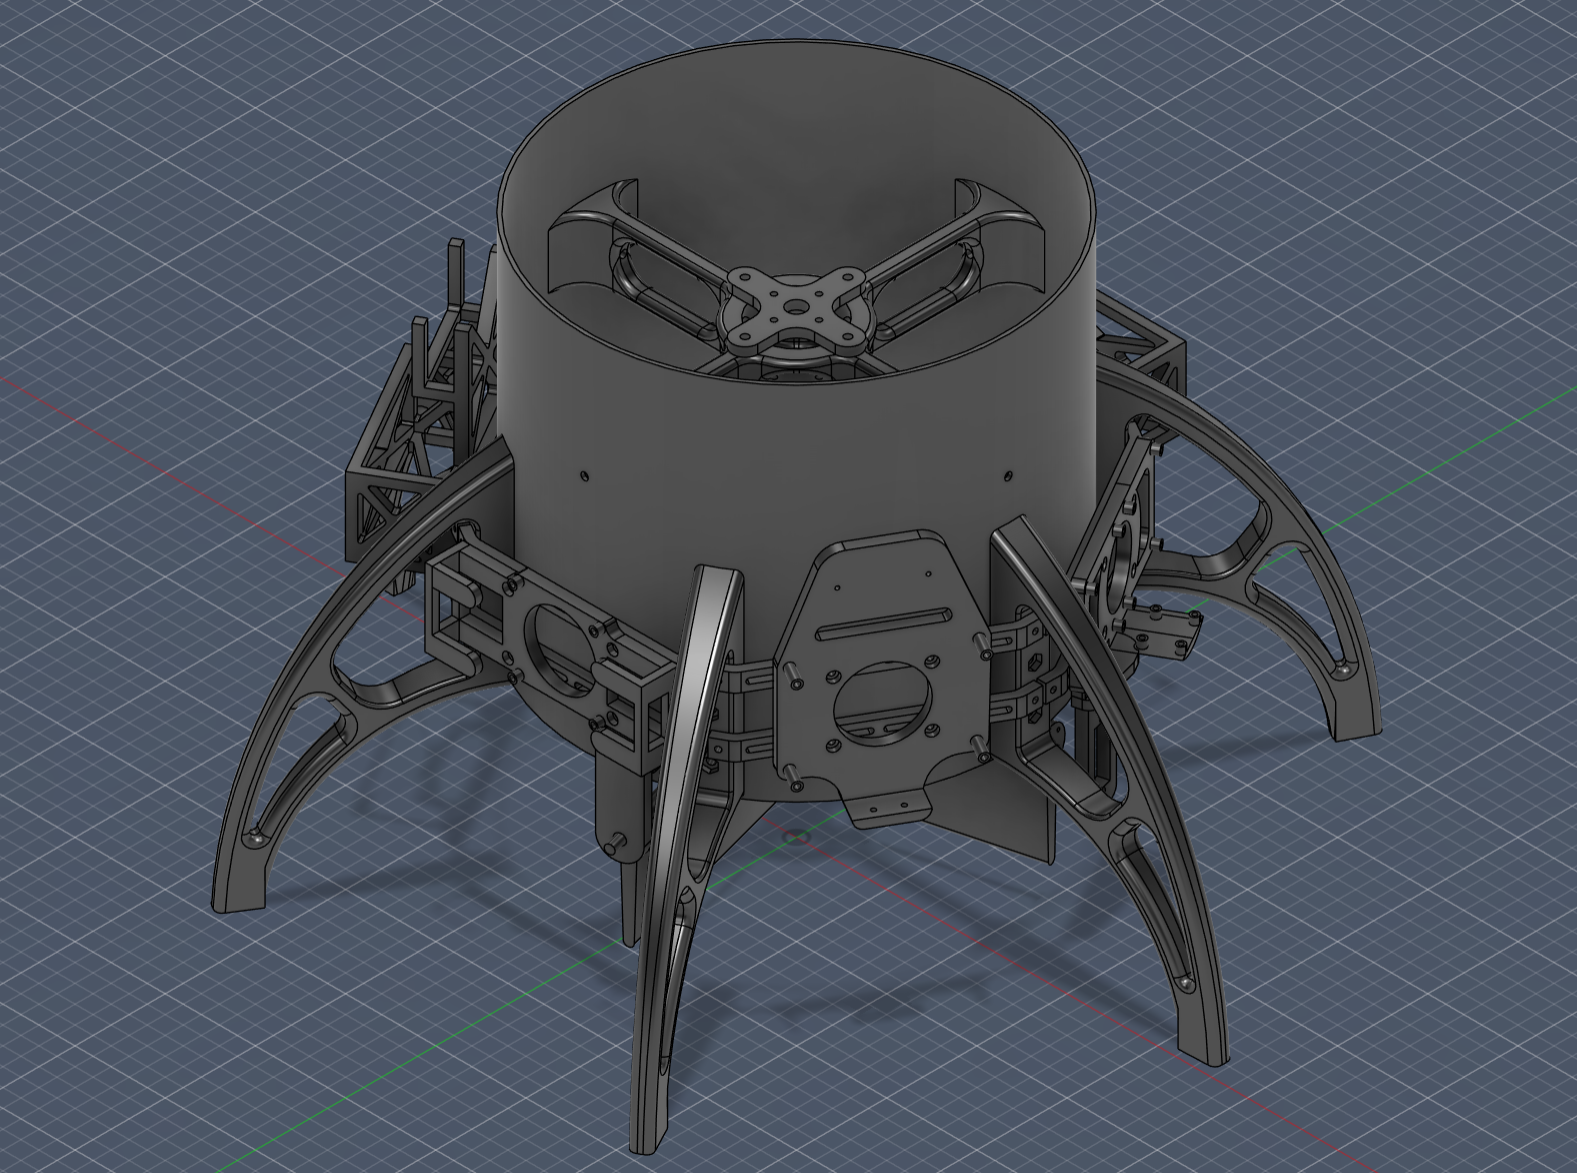
\includegraphics[height=5.4cm,keepaspectratio]{figures/01_sistema/image_fusion_2.png}
			\caption{Render struttura: vista frontale}
		\end{subfigure}
		
		\vspace{0.5cm}
		
		\begin{subfigure}[t]{0.9\textwidth}
			\centering
			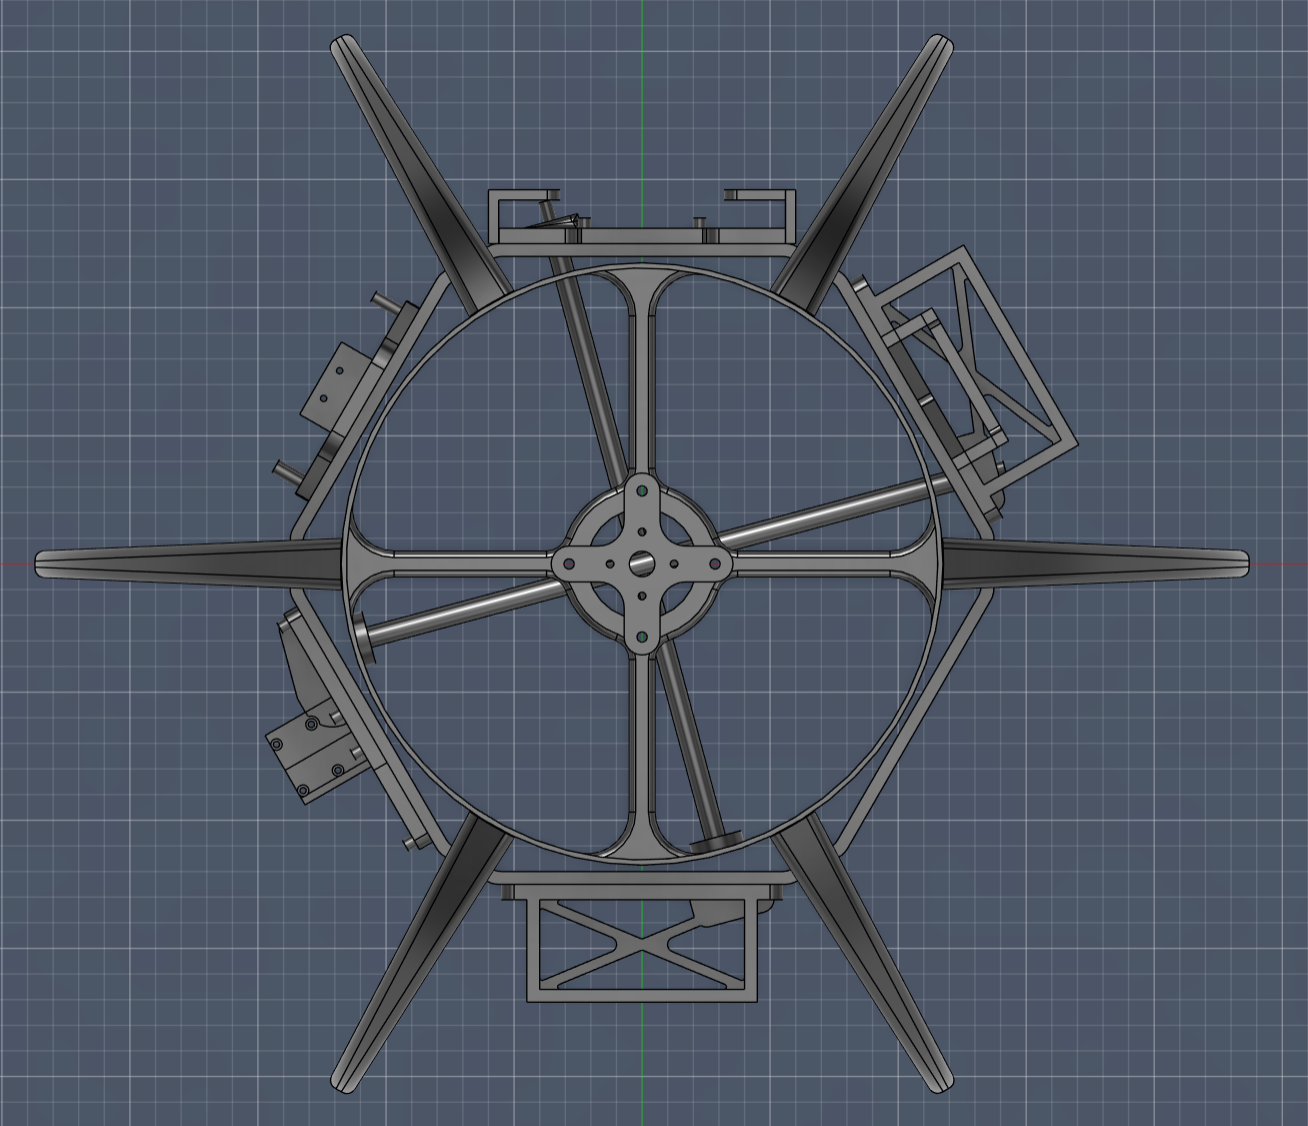
\includegraphics[height=5.4cm,keepaspectratio]{figures/01_sistema/image_fusion_3.png}
			\caption{Render struttura: vista dall'alto}
		\end{subfigure}
		\caption{\textcolor{black}{Render ducted fan}}
	\end{figure}
	
	\section{Controllo del Double Propeller Ducted-Fan}
	L'obiettivo di controllo del progetto è l'ottenimento dell'\textbf{hovering} del \textit{DPDF}. Con il termine \textit{hovering} si intende una condizione di volo stazionario in cui il velivolo mantiene quota e assetto prossimi ai valori desiderati, senza deriva apprezzabile nel breve intervallo temporale di osservazione.

	Dal punto di vista progettuale, questo obiettivo non viene affrontato come un unico problema monolitico, ma come la composizione di due sottoproblemi fisicamente distinti. Il primo è il controllo della \textbf{quota}, cioè dell'equilibrio tra peso e spinta verticale generata dai due propulsori. Il secondo è il controllo dell'\textbf{assetto}, cioè della soppressione delle rotazioni indesiderate attorno agli assi di \textit{roll} e \textit{pitch}, ottenuta deviando il getto d'aria tramite il comparto \textit{flap-servo}. Questa scomposizione è conveniente perché i due fenomeni sono osservati con sensori diversi, agiscono su attuatori diversi e presentano dinamiche caratteristiche differenti.

	Per questa ragione il firmware adotta un'architettura a tre regolatori PID: un anello dedicato alla quota, che modifica la portanza totale intervenendo in modo simmetrico sui due motori, e due anelli dedicati all'assetto, che generano l'angolo richiesto ai flap per contrastare gli errori di \textit{roll} e \textit{pitch}. La scelta dei PID non deriva da una preferenza generica per una soluzione nota, ma dal fatto che essi permettono di costruire un legame diretto e interpretabile tra errore misurato e azione correttiva, rendendo il comportamento del sistema abbastanza trasparente in fase di analisi sperimentale e di taratura.
	
	\newpage
	\chapter{Hardware}
	\label{Hardware}
	Nel presente capitolo viene fornita la descrizione di tutte le componenti hardware
	impiegate ai fini progettuali.
	Per ciascun componente sono stati approfonditi il ruolo nel sistema, le principali
	caratteristiche fisiche e tecniche e le modalità di utilizzo. Infine sono stati riportati un
	diagramma esplicativo dei collegamenti e una tabella riepilogativa delle connessioni.
	\section{STM32 NUCLEO-H745ZI-Q. La scheda di controllo}
	La scheda \textit{STM32 NUCLEO-H745ZI-Q} è una piattaforma di sviluppo prodotta da STMicroelectronics, basata sul microcontrollore STM32H745ZI-TQ6, appartenente alla famiglia ad alte prestazioni STM32H7. Il dispositivo è stato progettato per facilitare lo sviluppo, il \textit{debug} e la prototipazione di applicazioni \textit{embedded} complesse.
	La NUCLEO-H745ZI-Q è stata utilizzata per lo sviluppo e la fase di prova dei \textit{firmware} di gestione di tutte le componenti del \textit{DPDF}. Su di essa sono state caricate le librerie software sviluppate con l'ausilio di STM32CubeIDE.
	Segue una descrizione dettagliata delle principali caratteristiche del microcontrollore STM32H745ZI-TQ6.
	
	\subsection{STM32H745ZI-TQ6. Architettura}
	Il microcontrollore STM32H745ZI-TQ6 presenta un'architettura \textit{dual-core} a 32-bit composta da un processore ad alte prestazioni, il \textbf{Cortex-M7}, e da un processore il cui utilizzo è consigliato per applicazioni \textit{real-time} e \textit{low-power tasks}. L'architettura consente l'implementazione di applicazioni \textit{multithread}.
	In questo progetto di tesi, l'esecuzione delle librerie \textit{software} di gestione dei dispositivi interessati è affidata al \textbf{Cortex-M4}.
	La selezione e la configurazione delle periferiche dello \textit{STM32H745ZI-TQ6} necessarie al raggiungimento degli obiettivi progettuali verranno approfondite nel capitolo dedicato al \textit{firmware}.
	A seguire un elenco delle caratteristiche concernenti all'architettura \textit{dual-core}:
	\begin{itemize}
		\item Il \textbf{Cortex-M7} opera ad una frequenza di 480 MHz.
		\item Il \textbf{Cortex-M4} opera ad una frequenza di 240 MHz.
	\end{itemize}
	\begin{figure}[H]
		\centering
		\includegraphics[width=0.5\textwidth]{figures/02_hardware/architettura_stm32h745zi_tq6.png}
		\caption{\textcolor{black}{Il microcontrollore STM32H745ZI-TQ6}}
		\label{fig:stm32h745zi-tq6}
	\end{figure}
	
	
	\subsection{STM32H745ZI-TQ6. Memoria}
	Il microcontrollore possiede una struttura di memoria complessa e stratificata.
	Le memorie interne principali sono la memoria \textit{Flash} e la \textit{SRAM}. Inoltre, il \textit{core M7} monta una \textit{cache L1} e una piccola \textit{backup SRAM} alimentabile a batteria.
	
	\paragraph{\small{Flash}}\mbox{}\\
	La Flash interna da \textbf{2 MByte} è l'area di memoria su cui risiede il \textit{firmware}. La memoria in questione è organizzata in \textit{dual-bank}, che permette la programmazione/cancellazione di una banca dati mentre si esegue sull'altra.
	
	\paragraph{\small{SRAM}}\mbox{}\\
	Il dispositivo dispone di circa \textbf{1 MByte} di memoria dati volatile o SRAM, distribuita in più banchi con caratteristiche e destinazioni d'uso differenziate. In particolare:
	\begin{itemize}
		\item La SRAM1 e la SRAM2, rispettivamente da 320 KByte e 384 KByte, costituiscono i blocchi principali ad alta velocità, accessibili da entrambi i \textit{core}. Rappresentano l'area privilegiata per l'allocazione dei dati che richiedono tempi di accesso ridotti e condivisibilità tra i due processori.
		\item Il blocco di SRAM3, da 128 KByte, è tipicamente dedicato al \textbf{Cortex-M4}, favorendo così una separazione logica delle risorse riducendo anche i conflitti di accesso.
		\item SRAM4, SRAM5 e SRAM6, in ordine, 128 KByte, 64 KByte e 64 KByte completano la struttura, fornendo ulteriori spazi di memoria che possono essere destinati a funzioni specifiche o a buffer ad alte prestazioni, secondo esigenze applicative.
	\end{itemize}
	
	\paragraph{\small{Cache L1}}\mbox{}\\
	Il \textbf{Cortex-M7}, a supporto dell'efficienza complessiva, integra una \textit{cache L1} per istruzioni e dati, riducendo la latenza di accesso alla memoria non volatile e minimizzando i colli di bottiglia dovuti alla differenza tra la velocità del processore e quella della \textit{Flash}. In tal modo le prestazioni globali del sistema risultano incrementate.
	
	\paragraph{\small{Flexible Memory Controller e Dual-mode Quad-SPI}}\mbox{}\\
	Il \textit{Flexible Memory Controller} è un'unità hardware che consente l'interfacciamento diretto con memorie parallele esterne al dispositivo. Il \textit{FMC} supporta: SRAM, PSRAM, SDRAM, NOR Flash e NAND Flash. L'integrazione del \textit{FMC} comporta un incremento nell'efficienza delle comunicazioni. Una volta configurato il \textit{controller}, la memoria esterna entra a far parte dello spazio di indirizzi del microcontrollore mascherando la complessità del protocollo.
	Il \textit{Dual Mode Quad-SPI} è un'altra interfaccia dedicata alle \textit{Flash} seriali esterne ad alta velocità. La soluzione poco fa citata permette di espandere la memoria dedicata al \textit{firmware} oppure di archiviare dati.
	
	\paragraph{\small{Memory Protection Unit}}\mbox{}\\
	La \textit{Memory Protection Unit} è una componente hardware integrata in ciascun \textit{core} del microcontrollore. La mansione del circuito integrato in questione è quella di controllare e regolare l'accesso alla memoria.
	
	\paragraph{Unità di elaborazione}\mbox{}\\
	L'architettura dell'STM32H745ZI-TQ6 integra anche unità di elaborazione dedicate ai calcoli numerici e al processamento dei segnali.
	
	\paragraph{\small{Floating Point Unit}}\mbox{}\\
	La \textit{FPU} è un'unità hardware integrata nei due \textit{core} di elaborazione che consente l'esecuzione diretta di operazioni in virgola mobile. La presenza di questo circuito integrato riduce drasticamente la latenza di calcolo in applicazioni che richiedono elaborazioni numeriche complesse.
	Nel caso del \textit{\textbf{Cortex-M7}} la FPU supporta sia la \textit{single precision} che la \textit{double precision}, mentre il \textit{\textbf{Cortex-M4}} solo una FPU a precisione singola.
	
	\paragraph{\small{Digital Signal Processing}}\mbox{}\\
	Il \textit{Digital Signal Processing} è un supporto hardware per istruzioni dedicate all'elaborazione numerica di segnali digitali.
	
	\subsection{STM32H745ZI-TQ6. Convertitori}
	\paragraph{\small{Convertitori Analogici-Digitali}}\mbox{}\\
	Lo STM32H745ZI-TQ6 integra tre convertitori analogico-digitali \textbf{SAR ADC} (\textit{successive approximation analog-to-digital converter}) a 16 bit: ADC1, ADC2 e ADC3.
	I primi due, l'ADC1 e l'ADC2, sono \textit{tightly coupled}, cioè strettamente accoppiati, consentendo una sincronizzazione precisa delle conversioni. Questo approccio permette di ottenere alte frequenze di campionamento, precisione temporale e riduzione del carico computazionale del core. L'ADC3 invece è istanziato separatamente.
	La risoluzione può essere configurata a 16, 14, 12, 10 o 8 bit.
	
	\paragraph{\small{Convertitori Digitali-Analogici}}\mbox{}\\
	Il microcontrollore possiede 2 \textbf{DAC} indipendenti la cui risoluzione è a 12 bit.
	
	\subsection{STM32H745ZI-TQ6. Timer}
	I \textit{timer} sono periferiche hardware fornite dal microcontrollore per svolgere attività correlate al tempo.
	Lo STM32H745ZI-TQ6 fornisce 15 \textit{timer} di diverso tipo e 5 \textit{low power timer}. Alcuni di questi possono essere utilizzati per la generazione di segnali PWM.
	
	\subsection{STM32H745ZI-TQ6. Periferiche di comunicazione}
	Lo STM32H745ZI-TQ6 integra un insieme ampio e variegato di protocolli di comunicazione. Le periferiche possono essere raggruppate in tre categorie principali: comunicazione seriale, comunicazione veloce e interfacce multimediali speciali.
	Per quanto riguarda la comunicazione seriale, il microcontrollore supporta i protocolli: $I^{2}C$, USART/UART e SPI.
	Nell'ambito della comunicazione veloce e avanzata il dispositivo supporta i protocolli: CAN (\textit{Controller Area Network}), USB OTG, Ethernet MAC, SD/SDIO/MMC.
	L'integrazione delle interfacce multimediali consente la gestione di applicazioni audio, grafiche e visione artificiale: SAI (\textit{Serial Audio Interface}), DFSDM (\textit{Digital Filter for Sigma-Delta Modulators}) e DCMI (\textit{Digital Camera Interface}).
	
	\subsection{STM32H745ZI-TQ6. Eventi asincroni}
	Il microcontrollore offre la possibilità di gestire con efficacia ogni genere di \textit{interrupt} (evento asincrono) grazie all'integrazione di un'unità di elaborazione dedicata: il NVIC (\textit{Nested Vector Interrupt Controller}).
	
	
	\subsection{NUCLEO-H745ZI-Q. Caratteristiche della scheda}
	La NUCLEO-H745ZI-Q è la scheda di sviluppo (\textit{development board}) che proietta all'esterno tutte le funzionalità del microcontrollore poco fa descritto.
	
	\paragraph{Caratteristiche fisiche}
	\begin{itemize}
		\item Dimensioni: $133.34\times 70.00$ [mm].
		\item Peso: 120 [g].
	\end{itemize}
	
	\paragraph{ST-LINK/V3E}\mbox{}\\
	Lo ST-LINK/V3E è un'interfaccia hardware, gestita dal microcontrollore STM32F723, dedicata al collegamento tra elaboratore esterno e microcontrollore. Il modulo permette di caricare il compilato \textit{firmware} sul microcontrollore direttamente dalla porta USB Micro-B collegata al sistema di elaborazione.
	Il modulo permette, inoltre, di eseguire il \textit{debug} in tempo reale del codice caricato sull'\textit{MCU}.
	L'ST-LINK/V3E fornisce anche interfacce ausiliarie utili ai fini dello sviluppo.
	A seguire un breve elenco esplicativo di queste funzionalità aggiuntive:
	\begin{itemize}
		\item VCP (\textit{Virtual COM Port}): lo ST-LINK integra un’interfaccia di comunicazione
		che emula una porta seriale virtuale (da cui il nome Virtual COM Port, VCP),
		tramite connessione USB. In tal maniera, l’elaboratore riconosce lo ST-LINK
		come una porta COM standard.
		\item MSC (\textit{Mass Storage Class}): la scheda di sviluppo appare al sistema di elaborazione come una memoria esterna.
	\end{itemize}
	
	\paragraph{Alimentazione}\mbox{}\\
	La scheda di sviluppo offre diversi approcci per l'alimentazione:
	\begin{itemize}
		\item Alimentazione via USB Micro-B ST-LINK a 5V.
		\item Alimentazione via Jack esterno da 7-12V.
		\item Alimentazione tramite \textit{pin Vin} esterno a 3.3V.
	\end{itemize}
	Nonostante la presenza di diversi approcci di alimentazione e i differenti voltaggi, la tensione di alimentazione del microcontrollore è 3.3V, ottenuta attraverso regolatori interni.
	Sulla scheda di sviluppo sono presenti dei \textit{jumper}, ovvero dei piccoli interruttori meccanici che permettono di riconfigurare l'\textit{hardware} della scheda evitando di intaccare il \textit{firmware}. Si suggerisce di prestare attenzione alla configurazione dei \textit{jumper} qualora si volesse alimentare la scheda da ingressi diversi dal \textbf{COM1} o \textbf{MICRO-B ST-LINK}.
	
	\begin{figure}[H]
		\centering
		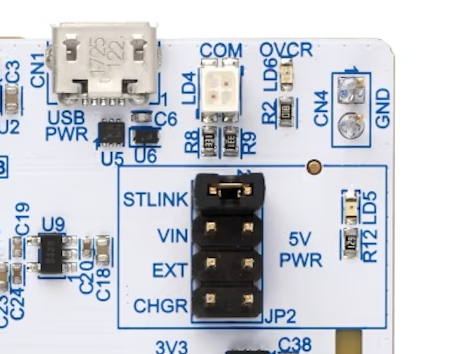
\includegraphics[width=0.6\textwidth]{figures/02_hardware/nucleo_h745zi_q_dettaglio_jumper.png}
		\caption{NUCLEO-H745ZI-Q. Dettaglio esplicativo dei \textit{jumper}}.
		\label{fig:nucleo-jumpers}
	\end{figure}
	
	\paragraph{Formato fisico}\mbox{}\\
	La scheda di sviluppo in esame appartiene alla famiglia \textbf{Nucleo-144} di STMicroelectronics e, dunque, mette a disposizione 2 connettori \textbf{\textit{Morpho}} che espongono i 144 \textit{pin} del microcontrollore. Il sistema di espansione poco fa citato viene chiamato ST Zio.
	La NUCLEO-H745ZI-Q offre, inoltre, la compatibilità hardware e pinout con gli \textit{shield Arduino Uno R3}.
	
	\begin{figure}[H]
		\centering
		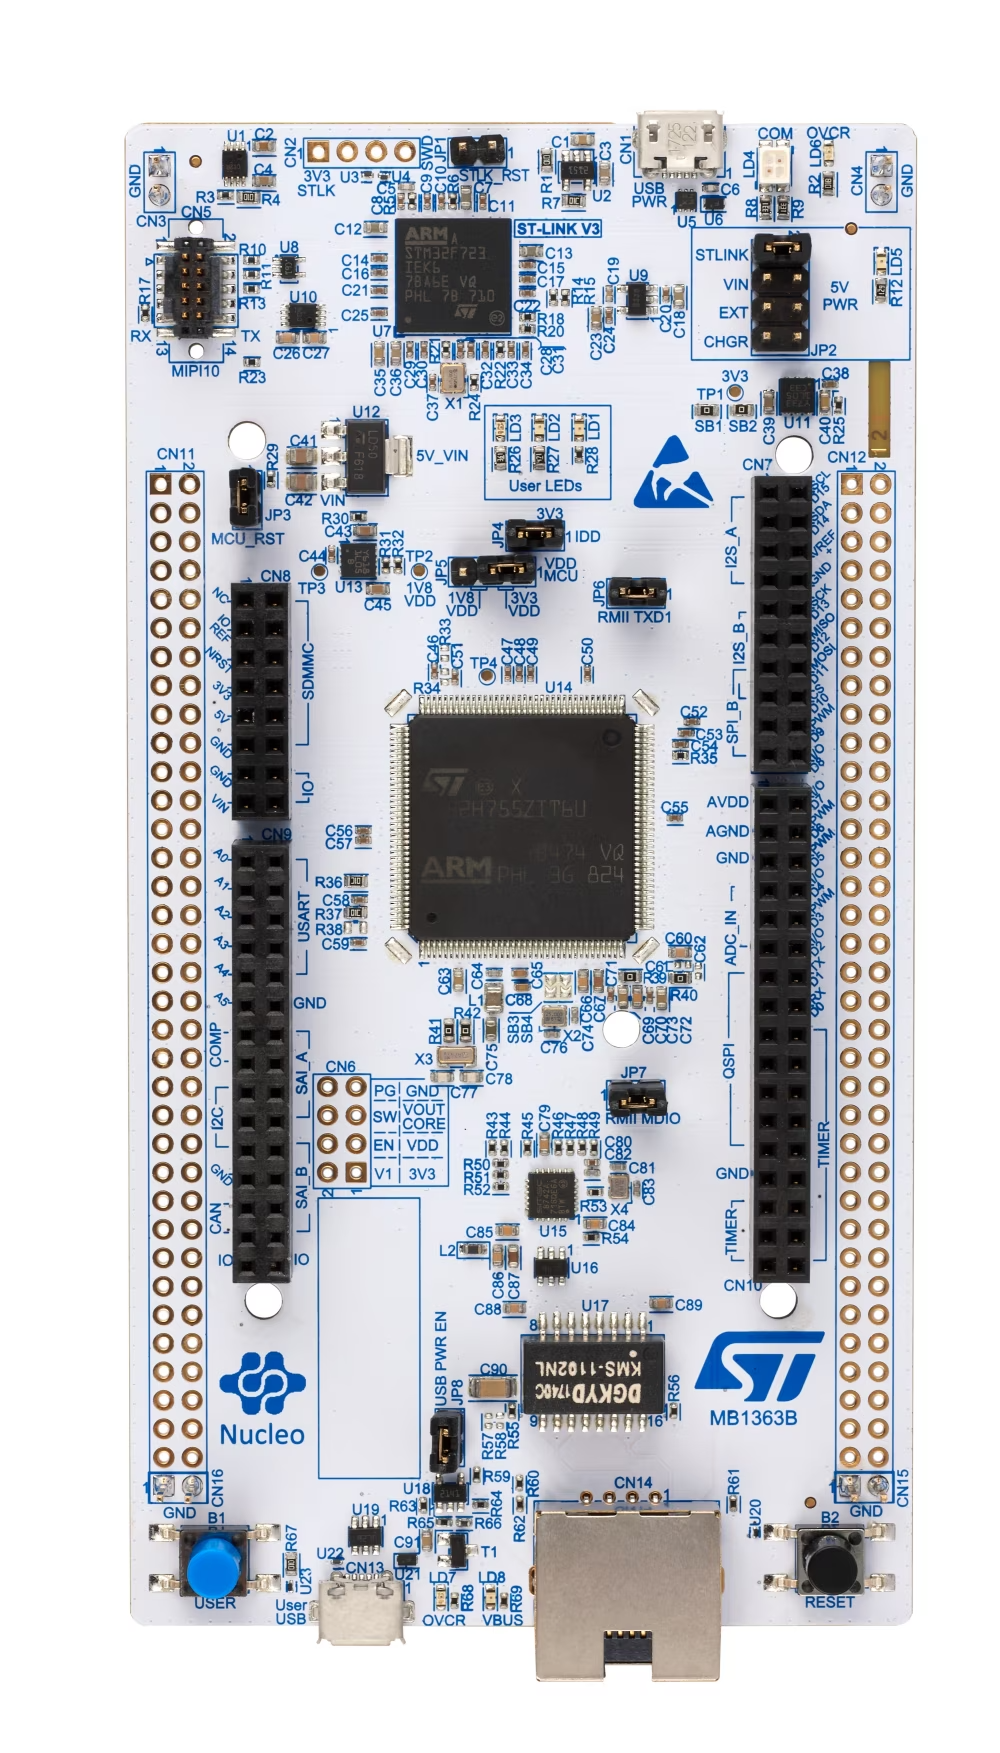
\includegraphics[width=0.6\textwidth]{figures/02_hardware/nucleo_h745zi_q_vista_superiore.png}
		\caption{\textcolor{black}{La scheda di sviluppo NUCLEO-H745ZI-Q}}
		\label{fig:nucleo-h745zi-q}
	\end{figure}
	
	
	\section{TATTU LiPo. Batteria ricaricabile}
	Motori, Servomotori e E.S.C richiedono specifici livelli di tensione per il loro funzionamento, tensioni che non possono essere fornite dalla NUCLEO H745ZI-Q.
	Si rende, quindi, necessario l'inserimento nel progetto di batterie ricaricabili.\\
	La selezione delle batterie disponibili sul mercato è stata condotta a seguito di un'analisi approfondita delle caratteristiche elettriche di motori, servomotori ed E.S.C,
	unitamente ad uno studio dettagliato delle esigenze di autonomia necessarie per le prove di volo, rapportando il tutto al \textit{budget} disponibile.\\
	Le \textbf{TATTU LiPo} possiedono le prestazioni richieste dal progetto.
	
	\subsection{TATTU LiPo. Caratteristiche fisiche}
	\begin{itemize}
		\item Dimensioni: $74\times 35.5\times 29$ [mm].
		\item Peso: 150 [g].
		\item Numero di celle: 4.
	\end{itemize}
	
	\subsection{TATTU LiPo. Caratteristiche tecniche e considerazioni operative}
	\paragraph{\small{LiPo}}\mbox{}\\
	La sigla \textit{LiPo} sta ad indicare la tecnologia elettrochimica utilizzata nella costruzione della batteria. \textit{LiPo} nasce da \textit{Lithium-Polymer}, ovvero polimero di litio.
	La particolare nominazione deriva dal componente chimico utilizzato come elettrolita, che, nel caso in esame, non è liquido, ma un polimero gelificato. Malgrado nelle fonti ufficiali non venga
	specificato il polimero usato nel progetto delle \textit{TATTU LiPo}, con il fine di informazione, è stato deciso di riportare quello più comunemente utilizzato per la tipologia di batterie in esame, il
	\textit{polivinilidenfluoruro esafluoropropilene} (PVDF-HFP).\\
	Rispetto ad altri sistemi elettrochimici presenti sul mercato (come ad esempio: Li-ion, $LiFePO_4$, NiMH ecc.), le batterie LiPo presentano un'elevata densità di potenza, una bassa resistenza interna e una
	notevole flessibilità nelle geometrie costruttive, oltre ad un contenuto peso. Tali attributi risultano vantaggiosi nell'ambito della progettazione di UAV, come il \textit{DPDF}.
	
	\paragraph{\small{Tensione}}\mbox{}\\
	La \textit{TATTU LiPo} possiede \textbf{4} celle da \textbf{3.7 [V]}. Le celle sono collegate in serie, perciò la tensione nominale è circa \textbf{14.8 [V]}.\\
	A carica completa, ogni cella può raggiungere i \textbf{4.2 [V]}, emettendo un'uscita di \textbf{16.8 [V]}.
	Il mantenimento della tensione delle celle nell'intorno dei 3.7 [V] contribuisce a preservare la stabilità chimica interna delle batterie,
	riducendo l'erosione delle celle e prolungandone la vita utile. Si consiglia di non mantenere le celle a 4.2 [V] per periodi prolungati di tempo, evitandone così il danneggiamento.\\
	Nella fase iniziale e di sviluppo \textit{firmware}, le batterie sono state tenute in bilanciamento alla tensione nominale di 14.8 [V], mentre,
	nella fase finale, in cui i \textit{test} di volo sono stati protagonisti, al fine di ottenere un aumento dell'autonomia delle batterie e della prestazione dei motori, queste venivano caricate, mantenendo il bilanciamento tra celle, fino a 4.2 [V] per cella.
	Infine, è necessario adottare un'ulteriore accortezza per evitare danni. È consigliabile non far scendere la tensione della batteria al di sotto dei \textbf{12 [V]}, mantenendo così il valore di tensione di ogni cella sopra i \textbf{3 [V]}.
	
	\paragraph{\small{Capacità}}\mbox{}\\
	La \textit{capacità} di una batteria, misurata in [mAh], \textit{milliAmpere-ora}, definisce la quantità di carica elettrica che la batteria può immagazzinare e fornire nel tempo.
	Nel caso in esame, la capacità è di \textbf{1300 [mAh]}, vale a dire che la batteria può fornire \textbf{1.3 [A]} per un'ora. In generale si può utilizzare la seguente formula approssimata per il calcolo del tempo di funzionamento:
	\begin{equation}
		t_h = \frac{C\,\,[mAh]}{A\,\,[mA]}
	\end{equation}
	dove $t_h$ rappresenta il tempo di funzionamento in ore, $C$ la capacità della batteria espressa in milliAmpere-ora e $A$ la corrente assorbita espressa in milliAmpere.
	Con il fine di aumentare l'autonomia di volo, si è optato per l'accoppiamento in parallelo di \textbf{due} \textit{TATTU LiPo}, così da ottenere una capacità totale di \textbf{2600 [mAh]}.
	L'accoppiamento in sicurezza è stato effettuato utilizzando il \textit{\textbf{PowerSafe Twin della MNR-electronics}}, il quale verrà approfondito nella successiva sezione.
	
	\paragraph{\small{Capacità di scarica}}\mbox{}\\
	Con il termine \textit{capacità di scarica} ci si riferisce alla quantità di corrente massima che la batteria può fornire, in sicurezza e in maniera continuativa, senza danneggiarsi.
	La \textit{TATTU LiPo} possiede una capacità di scarica pari a \textbf{75C}, vale a dire che può erogare:
	\begin{equation}
		A_{max} = C_s\cdot C \implies A_{max} = 75\,\,[C]\cdot 1.3\,\,[A]= 97.5\,\,[A]
	\end{equation}
	senza surriscaldarsi o danneggiarsi.\\
	Nella precedente formula, $A_{max}$ si riferisce alla corrente massima erogabile dalla batteria in sicurezza, espressa in [A], \textit{Ampère}. $C_s$ e $C$, invece, si riferiscono rispettivamente alla capacità
	di scarica e alla capacità di erogazione di corrente in un'ora, espressa sempre in [A].
	
	\begin{figure}[ht]
		\centering
		\captionsetup{margin=0pt}
		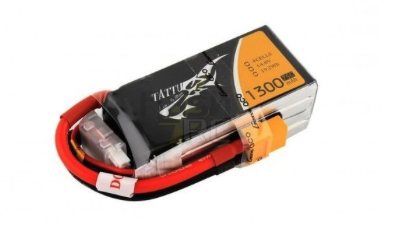
\includegraphics[width=0.6\textwidth]{figures/02_hardware/batteria_tattu_lipo_4s_1300mah_75c.jpg}
		\caption{TATTU LiPo 4S 1300mAh 75C}
		\label{fig:tattu-lipo}
	\end{figure}
	
	\section{PowerSafe Twin ADV. MNR-electronics}
	Per garantire la sicurezza e l'affidabilità dell'alimentazione a due pacchi batteria, si è deciso per l'implementazione del
	\textbf{modulo di ridondanza, PowerSafe Twin ADV di MNR-electronics}.\\
	Il dispositivo incarna un'avanzata soluzione di \textit{ridondanza attiva}. Quest'ultima fa riferimento alla capacità del sistema di intervenire attivamente nel funzionamento del circuito con il fine di garantire continuità di alimentazione.
	Il modulo, di fatto, monitora continuamente alcune variabili di stato, come tensione e corrente, selezionando, in tempo reale, il pacco alimentante il carico. Per esempio, se dovesse abbassarsi la tensione di una batteria sotto
	una certa soglia critica, il dispositivo commuterebbe automaticamente sull'altra, evitando così una significativa interruzione della potenza fornita.\\
	Nell'architettura del sistema è possibile distinguere tre moduli distinti.
	
	\paragraph{\small{Modulo di potenza}}\mbox{}\\
	Il modulo di potenza è il circuito elettrico responsabile della commutazione tra i pacchi batteria, del bilanciamento e della distribuzione di corrente verso il carico.\\
	Inoltre, il dispositivo implementa circuiti di protezione, isolando la sorgente guasta, qualora si dovesse presentare un malfunzionamento, ed evitando il trasferimento di corrente fra i pacchi batteria.
	
	\paragraph{\small{Modulo di controllo}}\mbox{}\\
	Il modulo di controllo rappresenta il "centro di comando" del dispositivo. L'implementazione di un microprocessore permette la continua misura di parametri decisionali fondamentali, quali: la tensione delle batterie, la corrente di carico
	e l'eventuale squilibrio. L'inserimento del modulo di controllo nell'architettura circuitale permette l'implementazione della, precedentemente citata, tecnologia di \textit{ridondanza attiva}.
	
	\paragraph{\small{Modulo di allarme}}\mbox{}\\
	Il modulo di allarme provvede alla segnalazione di eventuali guasti mediante emissioni luminose (LED) ed acustiche (Buzzer).
	
	\subsection{PowerSafe Twin ADV. Caratteristiche fisiche e tecniche}
	A seguire, un breve elenco delle caratteristiche fisiche e tecniche del dispositivo:
	\begin{itemize}
		\item Dimensioni con involucro protettivo: $80\times 59\times 26$ [mm].
		\item Peso, considerando sia l'involucro protettivo che i cablaggi (connettori XT60): 100 [g].
		\item Corrente massima gestibile: 100 [A] (in continua).
		\item Numero di celle per pacco batteria gestibili: $[3S-8S]$.
		\item Tensione massima ammessa in ingresso: $\approx 33.6$ [V]. Considerando il minimo 3.7 [V] e il massimo 4.2 [V] per cella: $[11.1\div 33.6]$ [V].
	\end{itemize}
	
	\begin{figure}[H]
		\centering
		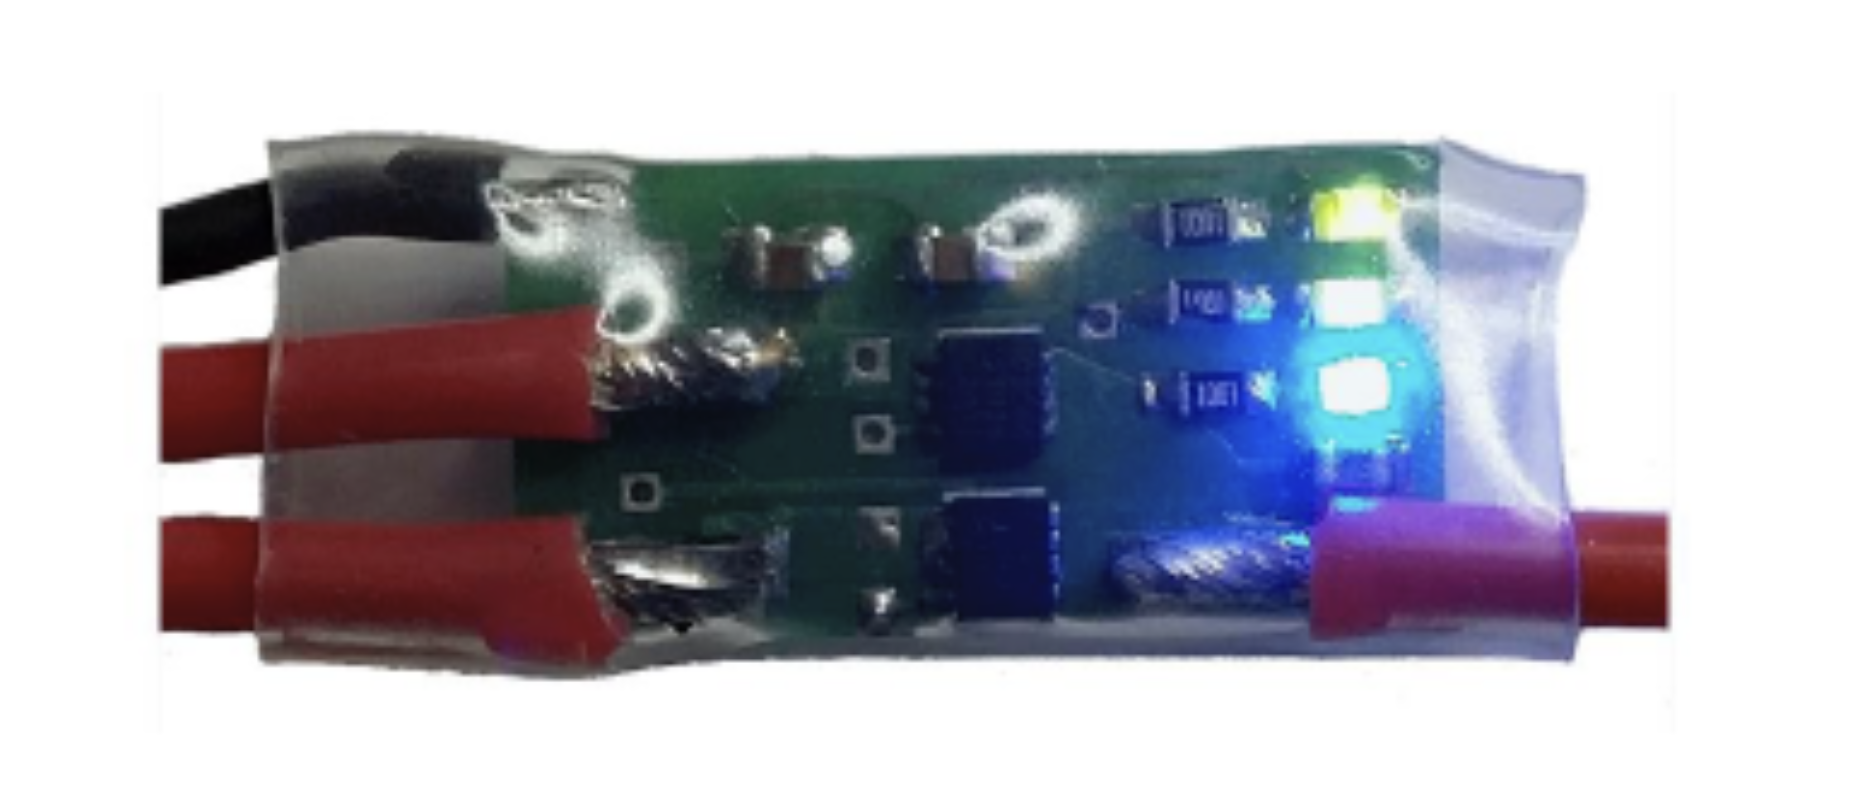
\includegraphics[width=0.6\textwidth]{figures/02_hardware/modulo_powersafe_twin_adv.png}
		\caption{PowerSafe Twin ADV MNR-electronics}
		\label{fig:powersafe-module}
	\end{figure}
	
	\section{DFRobot Power Module. Convertitore di tensione}
	Ai fini progettuali sono stati implementati diversi dispositivi, ciascuno dei quali richiedente una specifica tensione di alimentazione.
	Si è reso necessario ricorrere a convertitori di tensione per distribuire nella maniera corretta le tensioni di alimentazione ai vari dispositivi.\\
	Il \textbf{DFRobot Power Module} riceve in ingresso la tensione proveniente dal pacco batterie, erogando quattro diversi valori di tensione a seconda del terminale che si sceglie di utilizzare.\\
	La prima soluzione offerta dal dispositivo fornisce in uscita la stessa tensione che si ha in ingresso, diventando così un ponte per il passaggio della tensione.\\
	Un'altra soluzione consiste nell'utilizzo degli appositi \textit{pin} sul dispositivo, dai quali può essere erogata una tensione di \textbf{5 [V]}, selezionabile mediante un apposito \textit{switch}.\\
	Infine, il dispositivo presenta un terminale che eroga una tensione variabile il cui valore è controllato da un \textit{dimmer}. Il \textit{dimmer} permette di selezionare valori intermedi fino ad un massimo
	pari alla tensione di ingresso. Quest'ultima è stata utilizzata nell'alimentazione dei servomotori.
	La presenza di due servomotori ha richiesto l'integrazione di due convertitori di tensione.
	
	\begin{figure}[htbp]
		\centering
		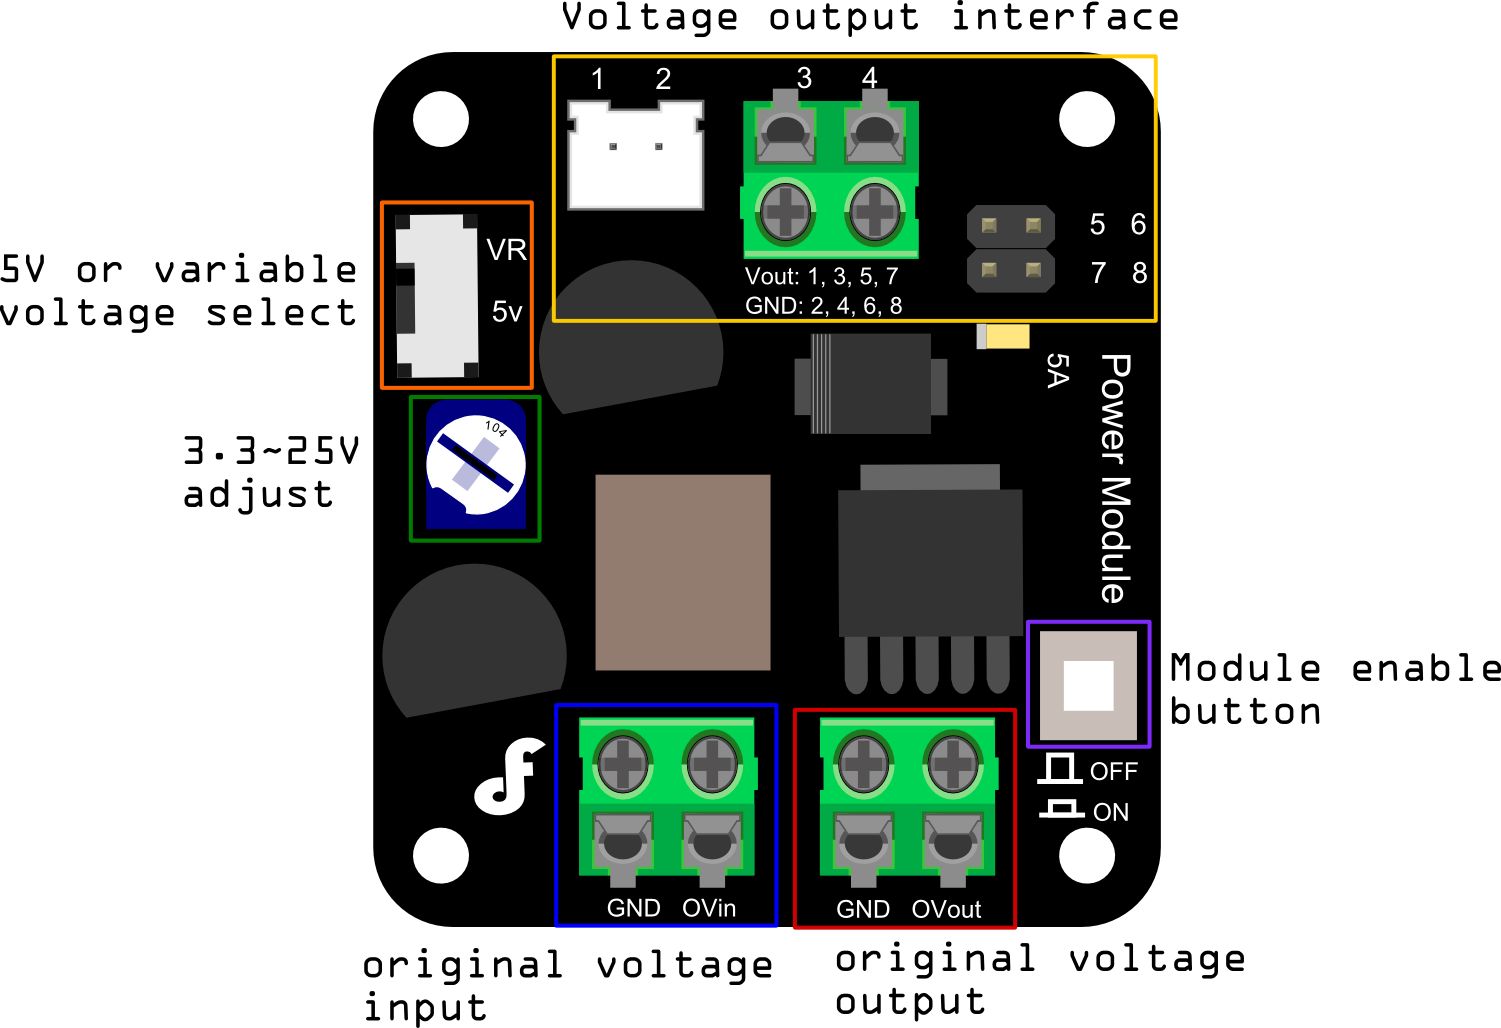
\includegraphics[width=0.5\textwidth]{figures/02_hardware/convertitore_tensione_dfrobot_terminali_uscita.png}
		\caption{DFRobot Power Module. Disposizione dei terminali di uscita}
		\label{fig:dfrobot-terminali}
	\end{figure}
	
	\paragraph{Caratteristiche fisiche}
	\begin{itemize}
		\item Dimensioni: $46\times 50\times 20$ [mm].
		\item Peso: 35 [g].
	\end{itemize}
	
	\paragraph{Caratteristiche tecniche}
	\begin{itemize}
		\item Intervallo di tensione in ingresso: \textbf{[3.6$\div$25] [V]}.
		\item Intervallo di tensione esprimibile in uscita: \textbf{[3.3$\div$25] [V]}.
		\item Massima potenza erogabile: \textbf{25 [W]}.
		\item Frequenza di variazione: \textbf{350 [kHz]}.
	\end{itemize}
	
	\begin{figure}[htbp]
		\centering
		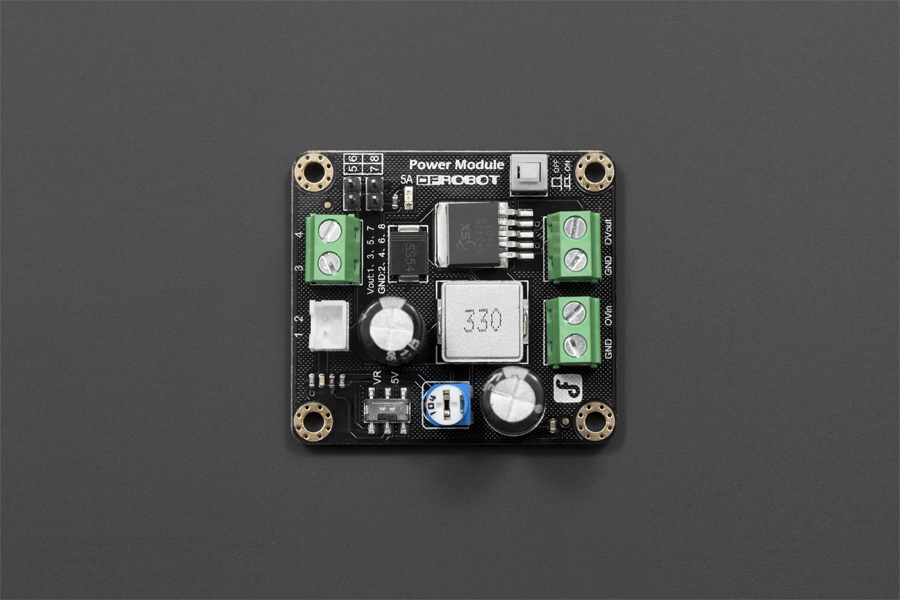
\includegraphics[width=0.6\textwidth]{figures/02_hardware/convertitore_tensione_dfrobot_foto_reale.jpg}
		\caption{DFRobot Power Module}
		\label{fig:dfrobot-modulo}
	\end{figure}
	
	\section{Power Distribution Board}
	Con \textbf{Power Distribution Board (PDB)} si fa riferimento ad un sottosistema elettrico la cui principale funzione è la \textbf{distribuzione in modo sicuro ed efficiente dell'energia fornita dal pacco batterie} agli \textit{E.S.C} e, conseguentemente, ai motori.
	Ai fini progettuali, è stata selezionata una \textit{PDB}, il cui punto di prelievo del segnale presenta un connettore \textbf{XT60}, adatto al pacco batterie.
	
	\begin{figure}[H]
		\centering
		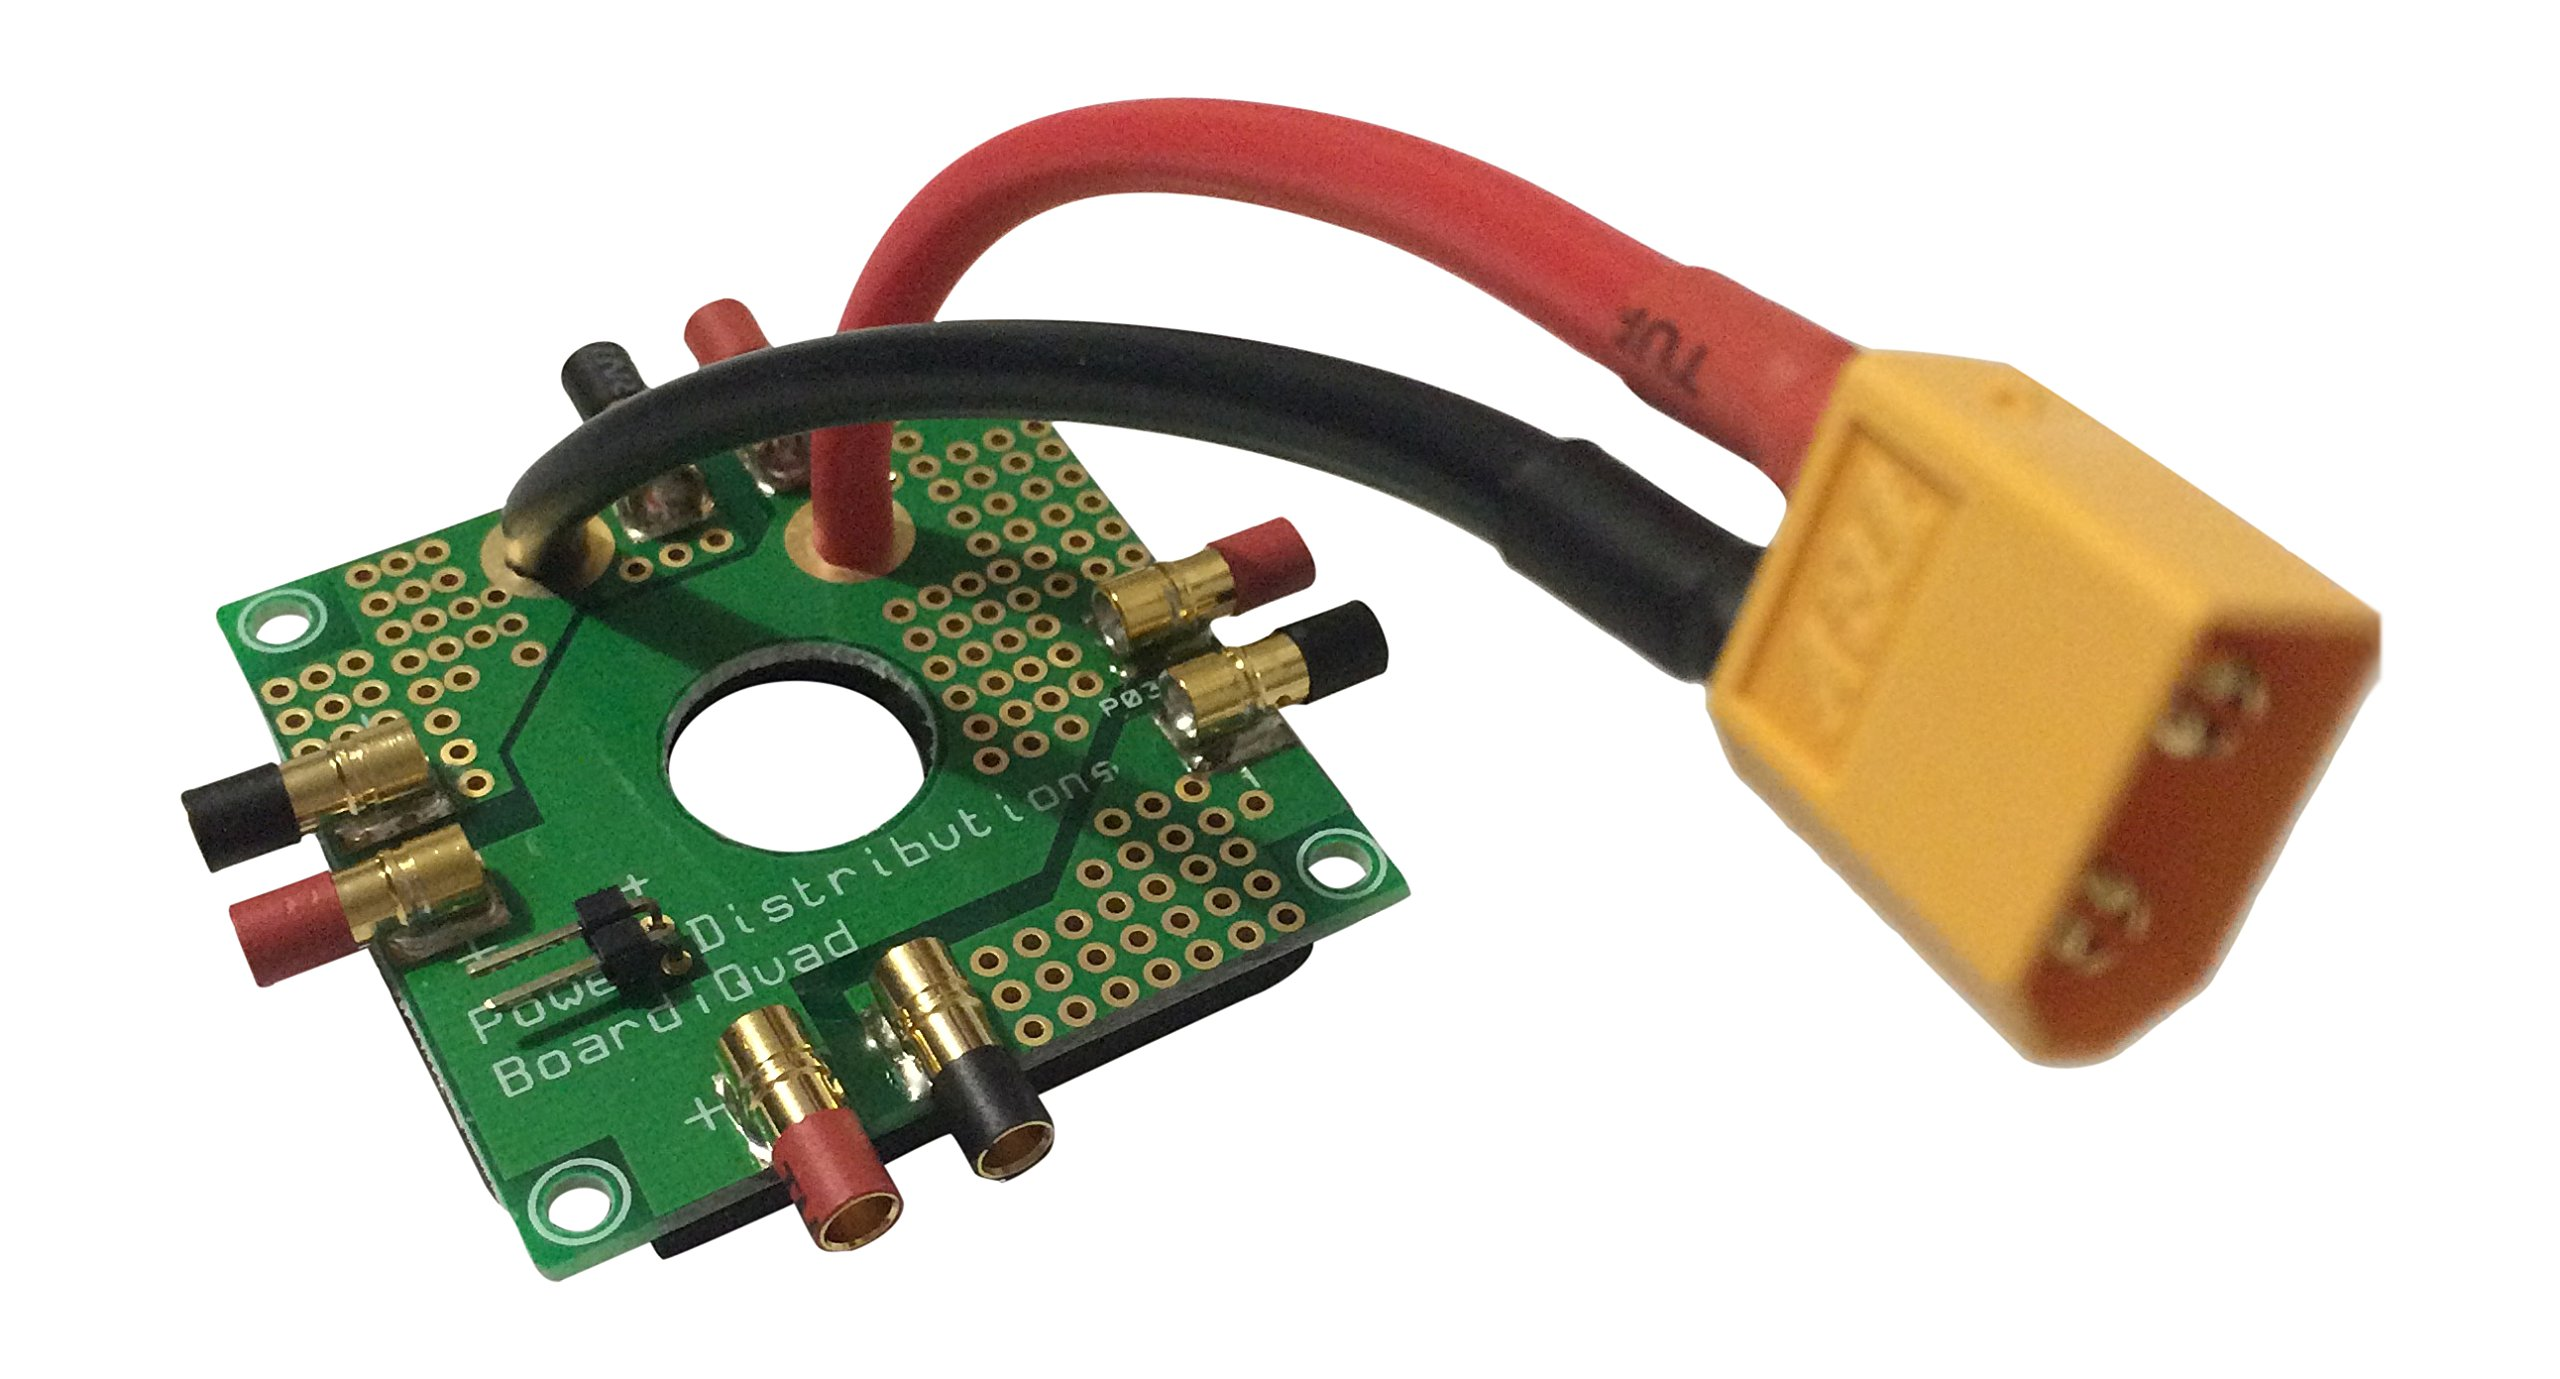
\includegraphics[width=0.6\textwidth]{figures/02_hardware/scheda_distribuzione_potenza_quad.jpg}
		\caption{Power Distribution Board}
		\label{fig:pdb}
	\end{figure}
	
	Il \textit{PDB} integrato nel contesto operativo possiede quattro uscite eroganti al massimo una corrente di \textbf{20 [A]} ed un peso di \textbf{27.3 [g]}.
	
	\section{Turnigy AereoDrive SK3-3536 1400KV}
	\label{MotoriBrushless}
	Il Turnigy AereoDrive SK3 3536 1400kv è un motore \textit{Brushless} alimentato a corrente continua e pilotato a trifase con correnti alternate.\\
	Il rotore contiene magneti permanenti disposti con polarità alternata lungo la sua circonferenza. Lo statore invece ospita tre avvolgimenti elettrici (fasi) disposti generalmente a 120 gradi elettrici l'uno rispetto all'altro, connessi ai tre terminali d'uscita che si identificano come A, B e C.\\
	Il rotore, essendo formato da magneti permanenti, non necessita di alimentazione: è lo statore a generare il campo magnetico rotante che induce il moto.\\
	Il cambio di polarità degli avvolgimenti deve essere gestito da un sistema elettronico esterno, \textit{l'Electronic Speed Controller (ESC)}, che nella successiva sezione verrà approfondito.\\
	I tre conduttori che fuoriescono dal motore rappresentano i terminali delle tre fasi dello statore. Ciascun filo è collegato a uno degli avvolgimenti e nessuno di essi costituisce un riferimento comune.
	Per far ruotare il motore è necessario che tali fasi vengano alimentate secondo una precisa sequenza temporale, generando un campo magnetico rotante.
	Se si dovessero scambiare due dei tre cavi, l'ordine di commutazione si invertirebbe con conseguente variazione del senso di rotazione.\\
	Nel progetto sono stati impiegati due motori del tipo precedentemente citato, disposti in configurazione \textbf{controrotante}, con il fine di compensare le rotazioni indesiderate di \textbf{yaw}.
	Tale scelta consente di bilanciare le coppie di reazione generate dalle eliche, riducendo il momento torcente sul velivolo. Inoltre, l'adozione di due motori si è resa necessaria in quanto un singolo
	attuatore non sarebbe stato in grado di generare una spinta sufficiente a garantire la portanza richiesta dal sistema nelle condizioni operative previste.
	
	\subsection{Turnigy AereoDrive SK3-3536 1400 KV. Caratteristiche fisiche e tecniche}
	\begin{itemize}
		\item Tensione operativa: \textbf{[11.1$\div$16.8] [V]}.
		\item Valore KV: \textbf{1400 $\left(\frac{RPM}{V}\right)$}.
		\item Potenza massima: \textbf{590 [W]}.
		\item Corrente massima: \textbf{40 [A]}.
		\item Resistenza interna: \textbf{[0.021$\div$0.025] [$\Omega$]}.
		\item Corrente a vuoto: \textbf{0.021 [A]}.
		\item Diametro dell'albero motore: \textbf{5 [mm]}.
		\item Peso: \textbf{111 [g]}.
		\item Spaziatura fori di montaggio: \textbf{25$\times$25 [mm]}.
		\item Connettori \textit{bullet} \textbf{da 3.5 [mm]}.
		\item Numero dei poli: \textbf{12}.
	\end{itemize}
	
	Il valore "KV" è comune nel contesto del modellismo ed indica il numero di giri al minuto (RPM) che il motore compie per ogni \textit{volt} applicato a vuoto, in formula:
	\begin{equation}
		RPM = KV\cdot V
	\end{equation}
	A tensioni di alimentazione maggiori rispetto a quelle specificate il motore rischia di assorbire troppa corrente e surriscaldarsi.\\
	I giri al minuto massimi dipenderanno dalla tensione applicata e dalle dimensioni delle eliche.\\
	Nel presente progetto, il motore in interesse deve essere alimentato a batteria, vale a dire in corrente continua, lasciando spazio alla necessità di un dispositivo che trasformi la tensione continua erogata dalle batterie in un segnale trifase a corrente alternata.
	Il dispositivo in questione è il precedentemente citato \textit{Electronic Speed Controller}.
	
	\begin{figure}[H]
		\centering
		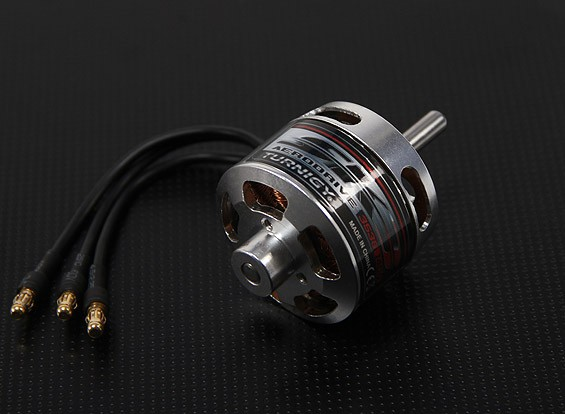
\includegraphics[width=0.5\textwidth]{figures/02_hardware/motore_turnigy_aerodrive_sk3_3536_1400kv.jpg}
		\caption{Turnigy Aereo Drive SK3 3536 1400 KV}
		\label{fig:turnigy-sk3}
	\end{figure}
	
	\section{Turnigy Plush 40A. \textit{Electronic Speed Controller}}
	Il Turnigy Plush 40A è un controllore elettronico di velocità per motori \textit{brushless} a corrente continua (BLDC) \cite{DCdriver}.\\
	Trasforma la tensione continua in ingresso in tensioni alternate sfasate di 120 gradi elettrici.\\
	L'applicazione della corretta sequenza di correnti alle fasi dello statore richiede la conoscenza della posizione angolare in ogni istante di tempo. Il Turnigy Plush 40A stima tale informazione in maniera indiretta, misurando la forza controelettromotrice indotta dal rotore, evitando così l'uso di sensori di posizione; il dispositivo in interesse può dunque essere definito \textit{sensorless}.
	L'ESC in questione può essere concettualmente suddiviso in due sezioni principali: la sezione di potenza e la sezione di controllo.
	La \textbf{sezione di potenza} è responsabile della conversione \textit{continua-trifase}. Tale conversione è mediata da un ponte trifase a sei MOSFET, suddiviso a sua volta in tre mezzi ponti, ciascuno associato ad una fase del motore.
	Ogni mezzo ponte è composto da un transistor di alto lato e da un transistor di basso lato, collegati rispettivamente al potenziale positivo della batteria e a massa. L'opportuna commutazione di apertura e chiusura dei sei MOSFET comporta la generazione di un segnale di tensione alternato per ogni fase.\\
	La \textbf{sezione di controllo} ha come protagonista un microcontrollore che si occupa della generazione di segnali di pilotaggio e della stima della posizione del rotore. Il microcontrollore riceve in ingresso il comando di velocità di rotazione del motore sotto forma di segnale PWM.
	Sulla base di tale comando, il microcontrollore determina il \textit{duty cycle} del PWM e calcola la sequenza di commutazione dei sei MOSFET, con conseguente generazione del campo magnetico rotante dello statore.\\
	Il \textit{Double Propeller Ducted Fan} monta due Turnigy Plush 40A, uno per ogni motore.
	
	\subsection{Turnigy Plush 40A. Caratteristiche fisiche}
	\begin{itemize}
		\item Corrente nominale: 40 [A].
		\item Corrente di picco: 55 [A].
		\item Presenza di un \textit{Battery Eliminator Circuit} (BEC): 5 [V] a 3 [A].
		\item Celle di batteria necessarie per il corretto funzionamento del dispositivo: $[2\div6]$.
		\item Peso: 39 [g].
		\item Dimensioni in [mm]: $60\times24\times15$.
	\end{itemize}
	
	\begin{figure}[H]
		\centering
		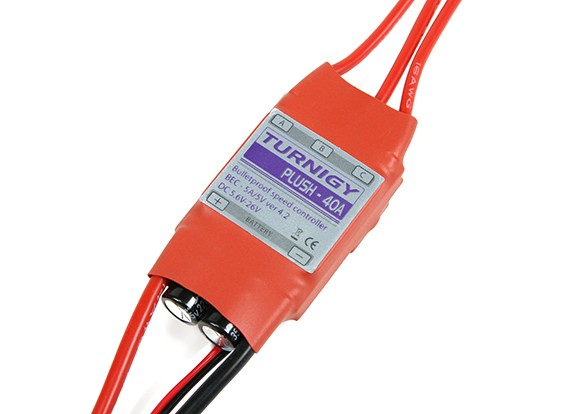
\includegraphics[width=0.6\textwidth]{figures/02_hardware/esc_turnigy_plush_40a.jpg}
		\caption{Turnigy Plush 40A}
		\label{fig:turnigy-plush-40a}
	\end{figure}
	
	\subsection{Turnigy Plush 40A. Programmazione}
	Il \textit{Turnigy Plush 40A} permette di configurare diversi parametri operativi del controllo motore. Nel progetto, entrambi gli ESC sono stati programmati tramite \textit{Turnigy Programming Card}, così da adattarne il comportamento alle esigenze del \textit{DPDF}.
	Per effettuare la programmazione è necessario predisporre i collegamenti elettrici mostrati in figura:
	
	\begin{figure}[ht]
		\centering
		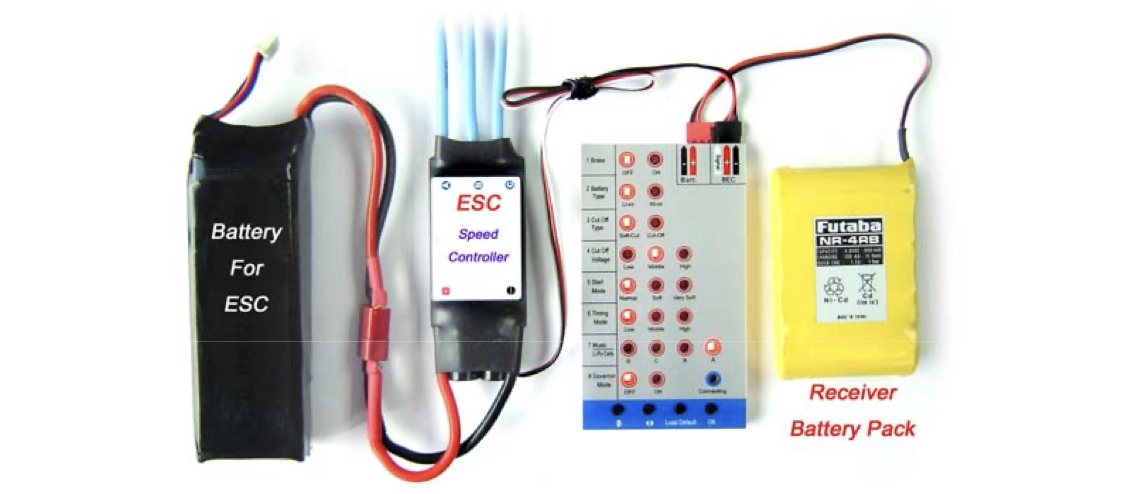
\includegraphics[width=0.6\textwidth]{figures/02_hardware/schema_collegamenti_programmazione_esc.png}
		\caption{Schema dei collegamenti per la programmazione dell'ESC}
		\label{fig:programmazione-esc}
	\end{figure}
	
	La \textit{Programming Card} è alimentata nell'intervallo $[4.8\div6]$ [V]; la navigazione fra i parametri avviene tramite i pulsanti \textit{up/down} e \textit{left/right}. Il LED \textit{connecting} segnala la corretta memorizzazione del parametro selezionato.
	Di seguito sono riportati i parametri principali e le impostazioni adottate.
	
	\paragraph{\small{Brake}}\mbox{}\\
	Il parametro \textit{Brake} definisce il comportamento del motore in assenza di segnale PWM. Poiché le prove sono state svolte in gabbia, questo parametro non è risultato determinante; è stato comunque impostato su \texttt{OFF}.
	
	\paragraph{\small{Battery Type}}\mbox{}\\
	Il \textit{Battery Type} informa l'ESC sul tipo di batteria utilizzata (LiPo o NiHM), così da gestire correttamente la protezione di bassa tensione. Poiché il sistema utilizza batterie \textbf{Tattu LiPo}, è stata selezionata l'impostazione \textit{Li-xx}.
	
	\paragraph{\small{Low Voltage Protection Mode (Cut-off Type)}}\mbox{}\\
	Questo parametro stabilisce come l'ESC reagisce quando la tensione di batteria scende sotto la soglia impostata. Per evitare arresti bruschi dei motori durante le prove, è stata scelta la modalità \textit{Soft Cut-Off}, che riduce progressivamente la potenza.
	
	\paragraph{\small{Cut Off Voltage}}\mbox{}\\
	Il parametro definisce la soglia di attivazione della protezione di bassa tensione:
	\begin{itemize}
		\item \textit{Low}: 2.85 [V];
		\item \textit{Medium}: 3.15 [V];
		\item \textit{High}: 3.3 [V].
	\end{itemize}
	È stata scelta l'impostazione \textbf{Medium}, che nel caso di una batteria LiPo a 4 celle corrisponde a una soglia complessiva di $11.4$ [V].
	
	\paragraph{\small{Start Mode}}\mbox{}\\
	La \textit{Start Mode} regola la rapidità con cui il motore accelera da fermo. Per limitare sollecitazioni meccaniche, movimenti bruschi ed errori di misura durante le prove in gabbia, è stata selezionata la modalità \textit{Soft Start}.
	
	\paragraph{\small{Timing Mode}}\mbox{}\\
	Il \textit{Timing} rappresenta l'anticipo con cui l'ESC commuta le fasi del motore rispetto alla posizione del rotore. Un valore basso privilegia efficienza e regolarità, uno alto favorisce potenza e velocità. Nel progetto è stata adottata la modalità \textit{Medium Timing}, in quanto compromesso tra prestazioni ed efficienza.
	
	\paragraph{\small{Music Li-Po Cells}}\mbox{}\\
	Questa funzione ha solo scopo estetico e non influisce sul comportamento del sistema; non è stata quindi utilizzata.
	
	\paragraph{\small{Governor Mode}}\mbox{}\\
	La \textit{Governor Mode} serve a mantenere costante la velocità del motore al variare del carico. Non essendo necessaria ai fini progettuali, è stata impostata su \texttt{OFF}.
	
	\begin{figure}[ht]
		\centering
		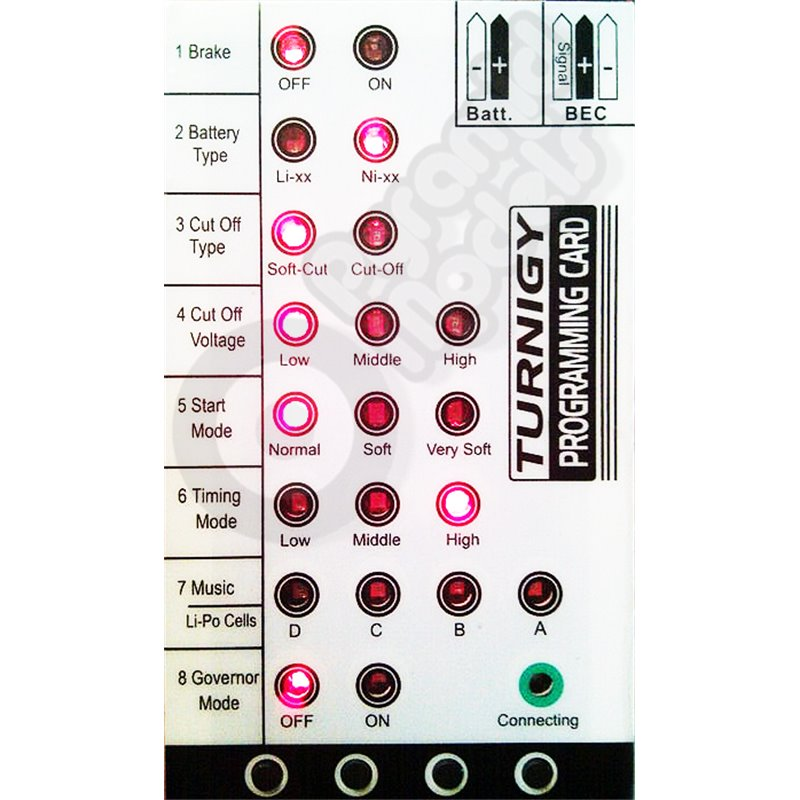
\includegraphics[width=0.6\textwidth]{figures/02_hardware/scheda_programmazione_turnigy.jpg}
		\caption{Turnigy Programming Card}
		\label{fig:turnigy-programming-card}
		\vspace{2mm}
		{\footnotesize L'immagine riportata sopra non è riferita alla configurazione attuale degli ESC, ma ha esclusivamente scopo illustrativo.}
	\end{figure}
	
	\subsection{Turnigy Plush 40A. Risoluzione e controllo dei motori}
	\label{ESCRisoluzioneEControllo}
	Il \textit{Turnigy Plush 40A} controlla i motori tramite un segnale PWM a $50$ [Hz], frequenza tipica delle applicazioni modellistiche. Prima del funzionamento è necessaria una procedura di armamento, ottenuta inviando un segnale con \textit{duty cycle} pari al $4.75\%$.
	L'esito dell'armamento può essere riconosciuto tramite le emissioni acustiche dell'ESC.
	
	\paragraph{\small{Attesa di un segnale di armamento valido}}\mbox{}\\
	Un'emissione sonora ogni due secondi indica che l'ESC è alimentato ma non ha ancora ricevuto un segnale PWM valido per l'armamento.
	
	\paragraph{\small{Esito positivo dell'operazione di armamento}}\mbox{}\\
	Tre segnali brevi seguiti da un segnale prolungato indicano che la procedura di armamento è andata a buon fine.
	
	\paragraph{\small{Esito negativo dell'operazione di armamento}}\mbox{}\\
	Una rapida sequenza di segnali acustici segnala invece un errore di armamento, generalmente dovuto a un segnale iniziale non corretto o a una variazione troppo rapida del \textit{duty cycle}. In base alle prove effettuate, è consigliabile attendere $[2\div6]$ [s] prima di aumentare il comando e l'intervallo di lavoro utile dei motori è risultato compreso tra $[6\%\div12\%]$.
	
	\paragraph{Risoluzione}\mbox{}\\
	Nel caso degli ESC, la ``risoluzione'' è intesa come intervallo di valori PWM distinguibili dal dispositivo. Questa informazione sarebbe utile per determinare la minima variazione di comando applicabile ai motori.
	Per il \textit{Turnigy Plush 40A} la documentazione ufficiale non fornisce un valore certo; alcune fonti non ufficiali indicano una risoluzione compresa tra 8 e 12 bit. A causa di questa incertezza, lo sviluppo del controllore è stato impostato in modo da non dipendere esplicitamente dalla risoluzione dell'ESC.
	
	\section{Eliche}
	Al fine di ottenere una corretta realizzazione progettuale, si rende necessario un minuzioso studio delle eliche da utilizzare.
	Le eliche e i motori costituiscono un perfetto connubio: se si dovessero scegliere eliche non adeguate, potrebbe non verificarsi la generazione della portanza necessaria al sollevamento del \textit{DPDF}.\\
	I parametri fondamentali per selezionare un'elica sono il \textbf{diametro} e il \textbf{passo}.\\
	Con il primo si indica il diametro della circonferenza che l'elica descrive durante la rotazione. Con il secondo, invece, si fa riferimento alla distanza teorica che l'elica percorrerebbe lungo il proprio asse in una singola rotazione completa, assumendo un fluido perfettamente solido e assenza di slittamento.
	Per chiarire il concetto, si può pensare a una vite che compie un giro completo mentre viene inserita nel legno.
	
	Il \textbf{diametro} di un'elica ne influenza:
	\begin{itemize}
		\item \textbf{Spinta}. Un aumento del diametro comporta un aumento della spinta a parità di RPM.
		\item \textbf{Efficienza}. Un aumento del diametro suggerisce un, seppur leggero, aumento dell'efficienza aerodinamica, dal momento che viene mosso un volume d'aria maggiore con una minore velocità del getto.
		\item \textbf{Coppia del motore richiesta}. A parità di regime di rotazione, eliche con diametro maggiore oppongono una coppia più elevata da parte del motore per essere mantenute in rotazione. Questo effetto non è in contrasto con il miglioramento dell'efficienza sopra descritto, poiché riguarda lo sforzo necessario a sostenere un determinato RPM, non la potenza richiesta per generare la medesima spinta.
		\item \textbf{Reattività}. Più è alto il valore del diametro e più è alta l'inerzia rotazionale, diminuendo la reattività del sistema.
	\end{itemize}
	Un elevato diametro è consigliato per sistemi che hanno l'obiettivo di stabilità.
	Per quanto riguarda il \textbf{passo}, il parametro influisce su:
	\begin{itemize}
		\item \textbf{Velocità in volo orizzontale}. Un aumento del passo costituisce un aumento della velocità espressa orizzontalmente.
		\item \textbf{Spinta}. La spinta espressa dall'elica aumenta se se ne aumenta il passo; tuttavia, il diametro dell'elica ha un'influenza maggiore.
		\item \textbf{Coppia del motore richiesta}. Un maggior passo richiede una maggior coppia indotta dai motori, con conseguente aumento dello stress meccanico.
		\item \textbf{Bassa efficienza di hovering}. Un aumento del passo comporta un aumento della velocità dell'aria mossa dall'elica, con conseguente diminuzione della stabilità.
	\end{itemize}
	Al contrario, un elevato passo è tipico dei sistemi focalizzati sulla velocità orizzontale e verticale.
	
	\subsection{APC 9x4.5. Caratteristiche fisiche}
	I dati riportati in \cite{Relazione1} indicano le seguenti caratteristiche fisiche:
	\begin{itemize}
		\item Diametro: 9 [in], pari a 228.6 [mm].
		\item Passo: 4.5 [in], pari a 114.3 [mm].
		\item Peso: 17.9 [g].
		\item Materiale: Nylon rinforzato con fibra di vetro (\textit{Fiberglass-Reinforced Nylon, FRN}).
	\end{itemize}
	
	\begin{figure}[H]
		\centering
		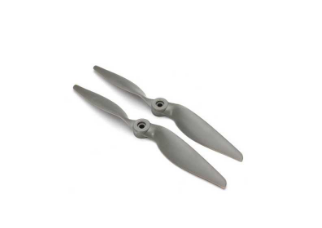
\includegraphics[width=0.55\textwidth]{figures/02_hardware/elica_apc_9x4_5.png}
		\caption{Elica APC 9x4.5}
		\label{fig:apc-9x45}
	\end{figure}
	
	\section{Hitec HS-82MG Gear micro servo}
	\label{HitecHS82MG}
	Il disegno strutturale rende il \textit{DPDF} suscettibile a rotazioni indesiderate sul piano definito dagli assi X ed Y. Tali perturbazioni possono compromettere la stabilità del sistema, determinandone una completa perdita di controllo del mezzo.\\
	Al fine di limitare tali perturbazioni, sono stati integrati due \textit{flap}, uno relativo al controllo lungo l'asse delle ascisse e uno lungo l'asse delle ordinate.\\
	I \textit{flap} operano come superfici aerodinamiche di controllo dedicate alla compensazione dei disturbi di \textit{rollio} e \textit{beccheggio}. Sono posizionati sulla parte terminale del condotto ed interagiscono con il getto generato
	dai motori controrotanti. L'intervento si basa sulla modifica della direzione e della velocità del flusso d'aria spinto verso il basso.
	Nel progetto sono stati integrati due servomotori del tipo sopra citato, uno per ogni \textit{flap}.
	
	\subsection{HS-82MG Hitec. Caratteristiche fisiche}
	\begin{itemize}
		\item Dimensioni: $29.8\times 12.0\times 29.6$ [mm].
		\item Peso: 19.0 [g].
	\end{itemize}
	
	\begin{figure}[ht]
		\centering
		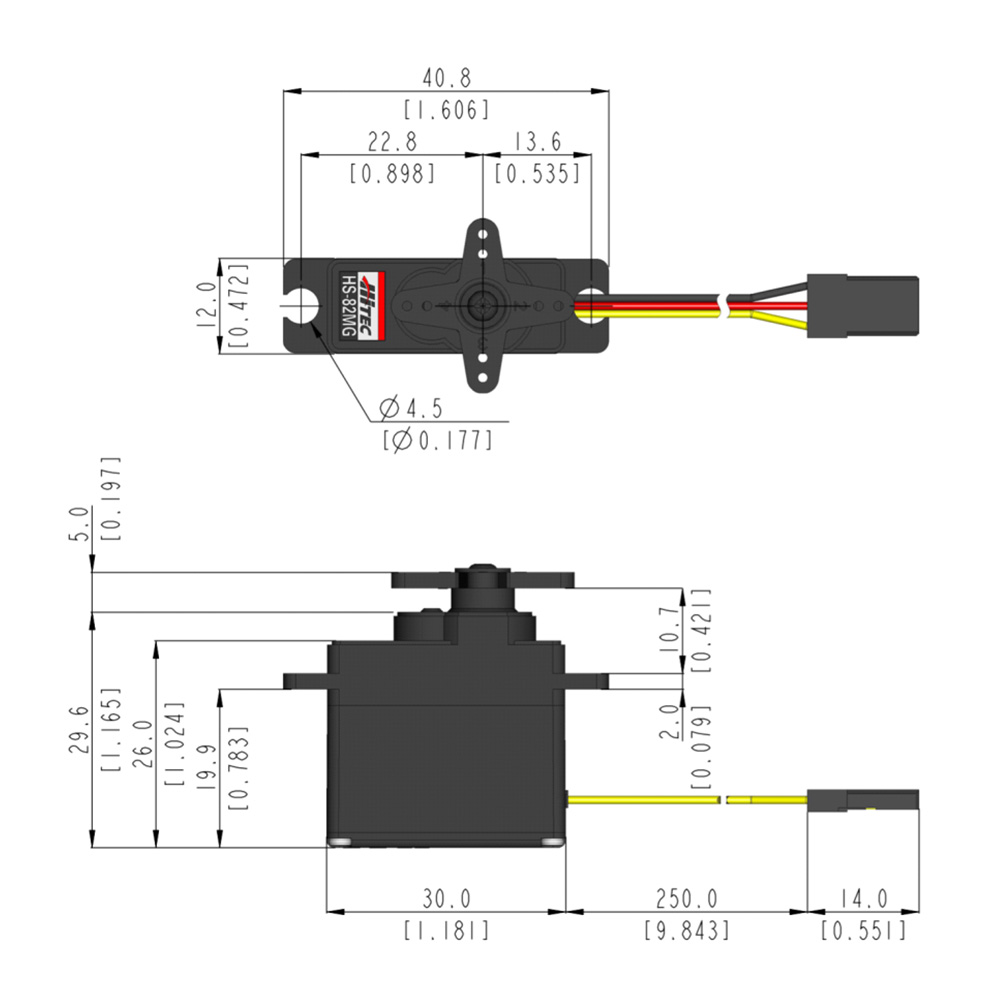
\includegraphics[width=0.4\textwidth]{figures/02_hardware/servo_hs_82mg_caratteristiche_fisiche.jpg}
		\caption{HS-82MG Hitec. Misure}
		\label{fig:hs82-misure}
	\end{figure}
	
	\paragraph{Coppia di stasi}\mbox{}\\
	Con \textit{coppia di stasi} si fa riferimento alla coppia massima che il servomotore può mantenere in posizione statica mentre oppone resistenza ad una forza esterna.\\
	L'\textit{HS-82} offre una coppia di stasi pari a: \textbf{2.2 [Kg$\cdot$cm]} con \textbf{4.8 [V]} in ingresso e \textbf{2.7 [Kg$\cdot$cm]} a \textbf{6.0 [V]}.
	
	\paragraph{Coppia di stallo}\mbox{}\\
	La coppia di stallo è la massima coppia teorica che il servomotore può generare a velocità angolare nulla, vale a dire con carico irremovibile.\\
	Per il dispositivo, la coppia di stallo assume i seguenti valori: \textbf{2.8 [Kg$\cdot$cm]} a \textbf{4.8 [V]} e \textbf{3.4 [Kg$\cdot$cm]} a \textbf{6.0 [V]}.
	
	\paragraph{Velocità angolare}\mbox{}\\
	La velocità angolare del dispositivo senza carico è di \textbf{60\degree\, in 0.12 [s]} a \textbf{4.8 [V]}, mentre è di \textbf{60\degree\, in 0.10 [s]} a \textbf{6.0 [V]}.
	Rapportando ad un singolo grado di variazione, si ha: \textbf{1\degree\, in 0.0020 [s]} a \textbf{4.8 [V]} e \textbf{1\degree\, in 0.0017 [s]} a \textbf{6.0 [V]}.
	
	\paragraph{Corrente operativa}\mbox{}\\
	La corrente operativa è la corrente assorbita dal servomotore mentre questo è in movimento. Le informazioni qui sotto riportate si riferiscono al servomotore privo di carico.\\
	Si ha un assorbimento di \textbf{220 [mA] per 60\degree} a \textbf{4.8 [V]} e un assorbimento di \textbf{280 [mA] per 60\degree} a \textbf{6.0 [V]}.
	
	\paragraph{Corrente di stallo}\mbox{}\\
	Con \textit{corrente di stallo} si fa riferimento alla massima corrente che il dispositivo assorbe quando è alimentato in condizione di blocco meccanico.
	Con questa configurazione, l'assorbimento di corrente ammonta a \textbf{1450 [mA]} a \textbf{4.8 [V]} e \textbf{1800 [mA]} a \textbf{6.0 [V]}.
	
	\paragraph{Corsa operativa}\mbox{}\\
	La \textit{corsa operativa} fa riferimento all'intervallo angolare che il servomotore copre in risposta ad un segnale PWM \textbf{standard}.
	Nel caso del \textit{HS-82}, l'intervallo è pari a \textbf{120\degree}.
	
	\begin{figure}[ht]
		\centering
		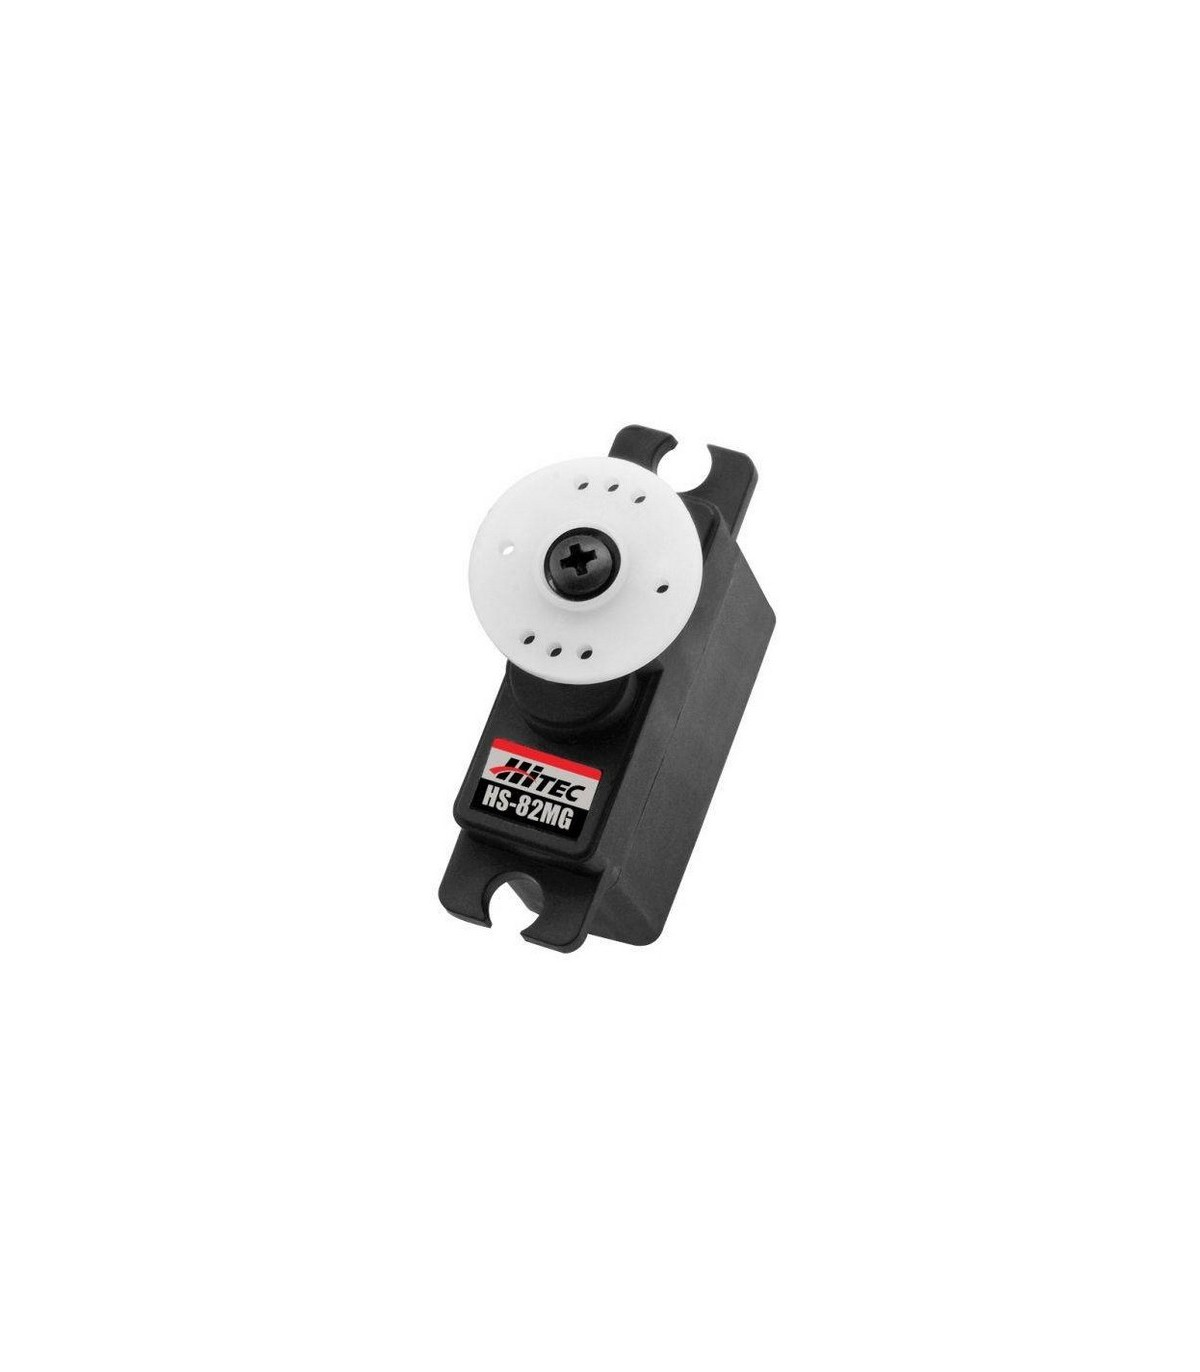
\includegraphics[width=0.6\textwidth]{figures/02_hardware/servo_hs_82mg_foto.jpg}
		\caption{HS-82MG}
		\label{fig:hs82-foto}
	\end{figure}
	
	\subsection{HS-82MG Hitec. Caratteristiche tecniche e controllo}
	\label{HS82ControlloAlimentazione}
	
	\paragraph{Alimentazione}\mbox{}\\
	L'intervallo di tensione operativa è il seguente: \textbf{[4.8$\div$6.0] [V]}.\\
	Per valori di tensione prossimi all'estremo superiore dell'intervallo si hanno dei miglioramenti sulle prestazioni generali del dispositivo. Tuttavia aumentano anche gli effetti dei comportamenti indesiderati, come un aumento della dispersione di calore per effetto Joule o dello stress sull'elettronica interna di controllo.\\
	Per evitare complicazioni, il valore di tensione in ingresso è stato impostato a \textbf{5.5 [V]}.
	
	\paragraph{Controllo}\mbox{}\\
	Il controllo della posizione angolare del rotore avviene tramite segnale PWM. Si è optato per una frequenza di \textbf{50 [Hz]}, mentre l'ampiezza è pari a \textbf{3.3 [V]}.
	Con il fine di ottenere il posizionamento dei \textit{flap} in configurazione perpendicolare al terreno, è necessario fornire un impulso di attivazione pari a \textbf{1.5 [ms]}. Con la frequenza scelta, tale valore corrisponde ad un \textbf{duty cycle del 7.5\%}, che rappresenta la posizione centrale del servomotore.\\
	La documentazione indica una \textit{Dead Band Width} pari a \textbf{5 [$\mu$s]}, ovvero la minima variazione di impulso che il servomotore è in grado di rilevare. Da ciò si deduce che la minima variazione angolare attuabile col servomotore è di \textbf{0.5\degree}. Nel contesto applicativo ciò equivale ad una variazione minima del \textit{duty cycle} pari a \textbf{0.025\%}.
	Per ottenere una rotazione oraria del rotore, il comando deve operare nel seguente intervallo di impulsi: \textbf{1.5$\div$2.1 [ms]}. L'effetto di rotazione antioraria si ha per: \textbf{0.9$\div$1.5 [ms]}.
	Analizzando il dato di velocità dei servomotori, è possibile determinare il tempo necessario affinché il servo compia la minima variazione angolare. Da questa informazione si può calcolare la frequenza massima di variazione della posizione del rotore, che si aggira intorno ai \textbf{400 [Hz]}.
	
	\begin{figure}[ht]
		\centering
		
\includegraphics[width=0.7\textwidth]{figures/02_hardware/servo_hs_82mg_collegamenti_elettrici.png}
		\caption{HS-82MG Hitec. Disposizione dei terminali}
		\label{fig:hs82-terminali}
	\end{figure}
	
	\section{BNO055 Bosch Sensortec. Unità di misura inerziale e magnetometro}
	Al fine di controllare l'orientamento nello spazio del \textit{DPDF} mediante servomotori, si necessita dell'informazione di rotazione del sistema nello spazio di riferimento. Si richiede, dunque, un dispositivo
	capace di ottenere tale informazione. Il \textbf{BNO055} della casa \textbf{Bosch Sensortec}, con la sua accuratezza, è il miglior candidato per tale responsabilità.
	Il \textbf{BNO055} è un sensore di orientamento assoluto a 9 assi sviluppato da \textbf{Bosch Sensortec}.
	Il dispositivo è un \textit{System in Package} che integra un accelerometro triassiale a 14 bit, un giroscopio triassiale a 16 bit, un sensore geomagnetico triassiale e un
	microcontrollore Cortex $M0^+$ a 32 bit incaricato nell'eseguire il \textit{software di sensor fusion} integrato.\\
	Il \textit{software}, poc'anzi citato, combina i dati provenienti da accelerometro, giroscopio e magnetometro, fornendo: \textbf{Quaternioni, Angoli di Eulero come pitch, roll e yaw e Vettori di orientamento lineari e gravitazionali}.
	Nel presente progetto, il \textit{chip} BNO055 è stato acquistato con montaggio su \textit{scheda di breakout} incluso, dunque nel paragrafo sottostante sono state aggiunte sia le dimensioni/peso del modulo che le dimensioni/peso del chip.
	
	\subsection{BNO055 Bosch Sensortec. Caratteristiche fisiche}
	\begin{itemize}
		\item dimensioni del modulo: $20\times24\times2$ mm.
		\item dimensioni del chip: $3.8\times5.2\times1.1$ mm.
		\item massa del modulo: 3 g.
		\item massa del chip: $\approx 150 mg$.
	\end{itemize}
	
	\subsection{BNO055 Bosch Sensortec. Infrastruttura di alimentazione, comunicazione ed integrazione del sensore}
	\paragraph{\small{Alimentazione}}
	Il \textit{BNO055} dispone dei terminali \textbf{$V_{DD}$} e \textbf{$V_{DDIO}$}, dedicati rispettivamente all'alimentazione del sensore e delle interfacce digitali. I relativi intervalli di alimentazione sono \textbf{[2.4$\div$3.6] [V]} per $V_{DD}$ e \textbf{[1.7$\div$3.6] [V]} per $V_{DDIO}$. Nel modulo utilizzato, questi ingressi sono gestiti internamente dalla \textit{breakout board} tramite il terminale unico $V_{IN}$, alimentabile nell'intervallo \textbf{[2.4$\div$3.6] [V]}. Tra le modalità di alimentazione disponibili, nel progetto è stata scelta la \textbf{\textit{Normal mode}}.
	
	\paragraph{\small{Protocollo di comunicazione}}\mbox{}\\
	Il \textit{BNO055} supporta i protocolli seriali \textit{$I^{2}C$} e \textit{UART}; nel progetto è stato utilizzato esclusivamente \textit{$I^{2}C$}. Il sensore può operare sia in \textit{Standard Mode} a 100 [kHz] sia in \textit{Fast Mode} a 400 [kHz]. Sia il sensore sia la relativa \textit{breakout board} espongono i terminali \textbf{SDA} e \textbf{SCL} per la comunicazione digitale.
	\begin{figure}[ht!]
		\centering
		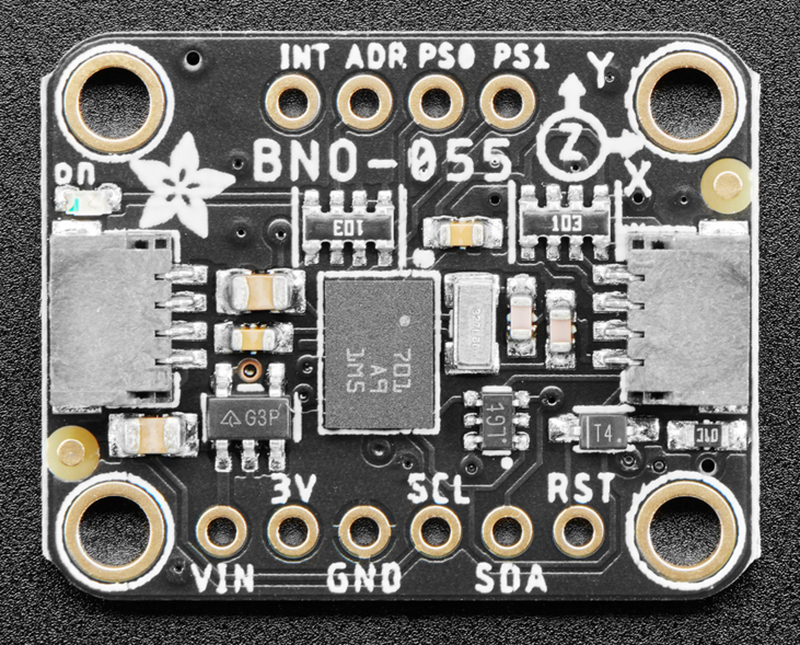
\includegraphics[width=0.4\textwidth]{figures/02_hardware/bno055_pinout_superiore.jpg}
		\caption{\textcolor{black}{BNO055 Bosch Sensortec. Configurazione dei pin e breakout board}}
		\label{fig:bno055-pinout}
	\end{figure}
	
	
	
	\subsection{Principio di misura dell'accelerometro, giroscopio e magnetometro}
	Prima di descrivere le caratteristiche del \textit{BNO055}, è utile richiamare sinteticamente il principio di funzionamento dei tre sensori che lo compongono.
	\paragraph{Accelerometro}\mbox{}\\
	L'accelerometro del \textit{BNO055} è un sensore capacitivo M.E.M.S. che misura l'accelerazione lungo i tre assi cartesiani. Il suo principio di funzionamento si basa sullo spostamento di una massa sospesa (\textit{proof mass}), che genera una variazione differenziale di capacità fra elettrodi fissi e mobili. Tale variazione viene convertita in segnale elettrico e successivamente digitalizzata.
	
	\paragraph{Giroscopio}\mbox{}\\
	Il giroscopio integrato è un M.E.M.S. vibrante che misura la velocità angolare sui tre assi. Il funzionamento si basa sull'effetto Coriolis: quando il sensore ruota, le masse vibranti interne subiscono una forza laterale proporzionale alla velocità angolare,
	\begin{equation}
		\vec{F_c}=2m(\vec{v}\times \vec{\omega })
	\end{equation}
	che viene rilevata come variazione di capacità e convertita in un segnale digitale.
	
	\paragraph{Magnetometro}\mbox{}\\
	Il magnetometro è basato sull'effetto Hall e misura il campo magnetico terrestre lungo i tre assi. La presenza di un campo magnetico perpendicolare alla direzione della corrente produce una tensione trasversale proporzionale al campo stesso. Questa tensione, dopo amplificazione e conversione analogico-digitale, fornisce le componenti cartesiane del vettore magnetico locale e permette di ricavare un riferimento assoluto di orientamento.
	
	\subsection{BNO055 Bosch Sensortec. Accelerometro, giroscopio e magnetometro integrati}
	Il \textit{BNO055} integra accelerometro, giroscopio e magnetometro Bosch Sensortec, combinandoli con un algoritmo interno di \textit{sensor fusion}.
	
	\paragraph{Accelerometro}\mbox{}\\
	L'accelerometro ha una \textbf{risoluzione di 14 bit} e supporta intervalli di misura pari a $[\pm 2]$ [g], $[\pm 4]$ [g], $[\pm 8]$ [g] e $[\pm 16]$ [g]. Nel progetto, con \textit{sensor fusion} attiva, viene utilizzato l'intervallo $[\pm 4]$ [g], adatto alla maggior parte delle applicazioni. In questa configurazione la banda passante è pari a \textbf{62.5 Hz}.
	
	\paragraph{Giroscopio}\mbox{}\\
	Il giroscopio ha una \textbf{risoluzione di 16 bit} e mette a disposizione intervalli di misura pari a $[\pm 125]$\degree/s, $[\pm 250]$\degree/s, $[\pm 500]$\degree/s, $[\pm 1000]$\degree/s e $[\pm 2000]$\degree/s. Con \textit{sensor fusion} attiva viene adottato l'intervallo $[\pm 2000]$\degree/s; pur essendo più rumoroso, consente di evitare saturazioni e il rumore viene compensato dall'elaborazione interna. La banda passante in questa modalità è \textbf{32 Hz}.
	
	\paragraph{Magnetometro}\mbox{}\\
	Il magnetometro misura campi fino a \textbf{$\pm 1300$ [\,$\mu$T]} sugli assi X e Y e fino a \textbf{$\pm 2500$ [\,$\mu$T]} sull'asse Z. La risoluzione è rispettivamente di \textbf{13 bit} e \textbf{15 bit}. Il sensore è sensibile a disturbi magnetici di tipo \textit{soft iron} e \textit{hard iron}, mitigati dall'uso della \textit{sensor fusion}. Con \textit{sensor fusion} attiva, la banda passante è \textbf{10 Hz}.
	
	\paragraph{Sensor fusion}\mbox{}\\
	Considerati singolarmente, i tre sensori presentano limiti complementari: il giroscopio è soggetto a deriva, l'accelerometro risente delle accelerazioni non gravitazionali e il magnetometro è vulnerabile ai disturbi magnetici ambientali. La \textit{sensor fusion} combina tali informazioni per ottenere una stima più stabile e affidabile dell'orientamento. Secondo la documentazione del \textit{BNO055}, l'elaborazione interna impiega un algoritmo di \textit{sensor fusion} che utilizza un \textbf{Filtro di Kalman esteso}; nel progetto questa modalità è stata mantenuta sempre attiva per migliorare attendibilità, accuratezza e stabilità della misura.\\
	A seguire una rappresentazione schematica del \textit{System in package BNO055 Bosch Sensortec}.
	\begin{figure}[ht!]
		\centering
		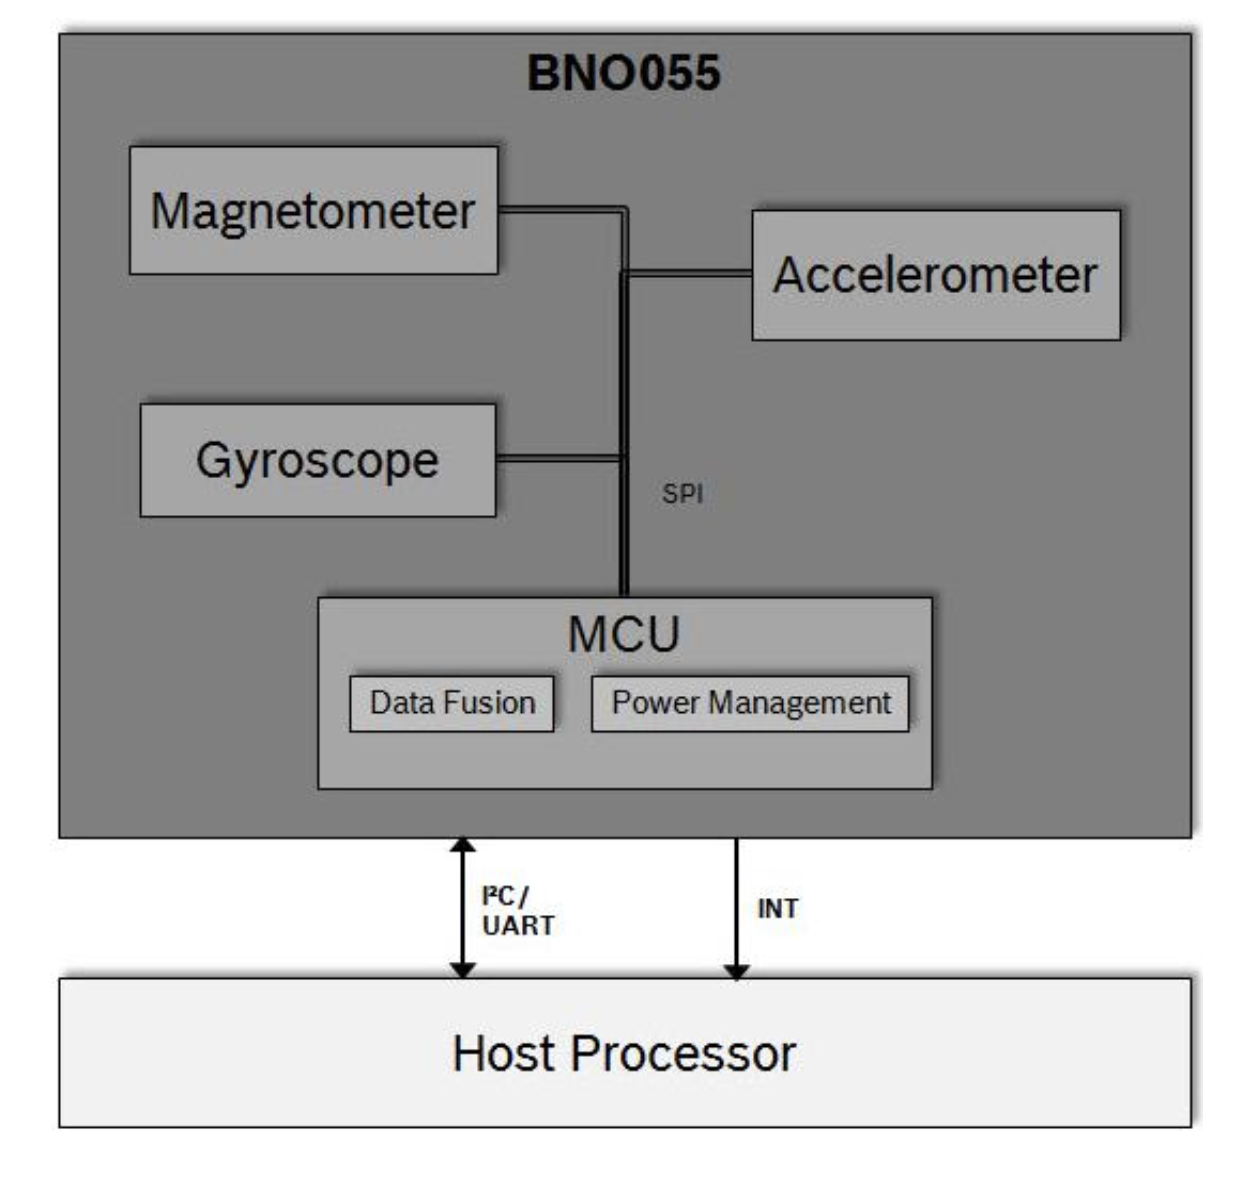
\includegraphics[width=0.4\textwidth]{figures/02_hardware/bno055_architettura_sistema.png}
		\caption{\textcolor{black}{BNO055 Bosch Sensortec. Architettura di sistema}}
		\label{fig:bno055-architettura}
	\end{figure}
	
	\subsection{BNO055 Bosch Sensortec. Modalità operative}
	Il dispositivo di misura fornisce una grande varietà di segnali di \textit{output}, che possono essere scelti selezionando l'appropriata modalità operativa.\\
	Le modalità operative vengono classificate in base all'attivazione o meno del \textit{software di sensor fusion}, nello specifico distinguiamo tra le \textit{Non-Fusion modes} e le \textit{Fusion modes}.
	\paragraph{Fusion-modes}\mbox{}\\
	Nel momento in cui viene impostata una delle seguenti modalità, l'algoritmo di fusione \textbf{esegue automaticamente, in \textit{background}, la calibrazione dei sensori}.
	\begin{itemize}
		\item \textbf{IMU (Inertial Measurement Unit)}. In questa modalità di fusione, l'orientamento relativo del \textit{BNO055} nello spazio, è determinato utilizzando i dati estratti dall'accelerometro e dal giroscopio. La computazione è veloce, di fatto è suggerita nelle applicazioni ad alta velocità.
		\item \textbf{M4G (Magnet for Gyroscope)}. Simile alla precedente modalità, tuttavia, il giroscopio non viene più utilizzato per la rilevazione della rotazione bensì la variazione dell'orientamento del magnetometro nel campo magnetico terrestre.
		\item \textbf{COMPASS}. In questa modalità, il \textit{BNO055} opera come una bussola elettronica, stimando l'orientamento sul piano orizzontale rispetto al nord magnetico. Rispetto alle modalità IMU e NDOF, che sfruttano il giroscopio per una risposta più pronta e stabile, questa modalità utilizza il magnetometro con consumi inferiori ma robustezza minore.
		\item \textbf{NDOF}. In questa modalità, la computazione dell'orientamento del dispositivo, è eseguita servendosi di tutti i dati provenienti dai sensori. La presente modalità è quella con il più alto consumo di corrente.
	\end{itemize}
	Nel presente progetto, la modalità \textbf{NDOF} è sempre stata scelta come modalità operativa del \textit{BNO055}.
	A seguire, un'immagine riportata dalla documentazione ufficiale, specificante la frequenza con cui il sensore produce dati in uscita, nel mentre che la \textit{sensor fusion} è attiva.
	\begin{figure}[ht!]
		\centering
		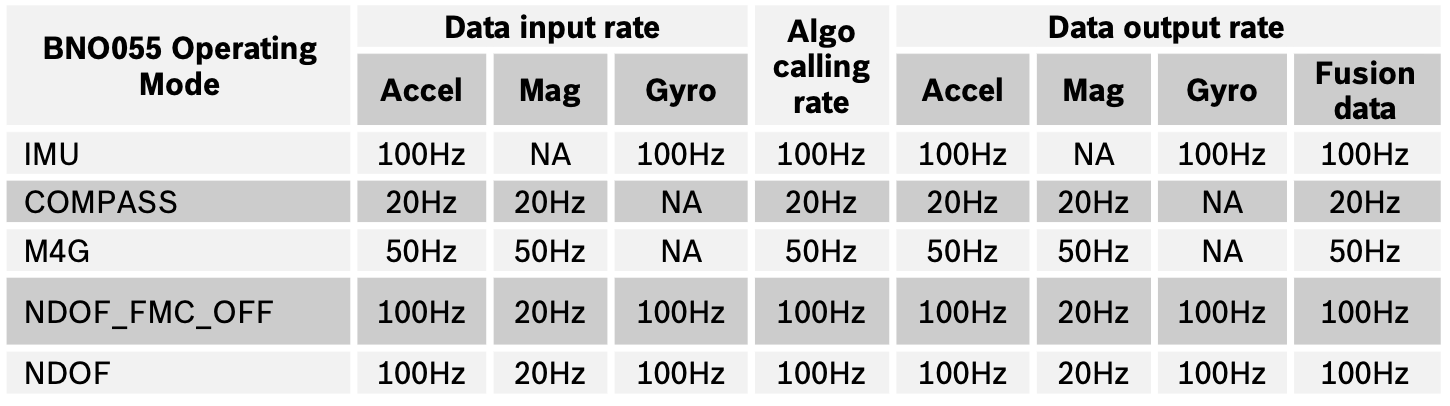
\includegraphics[width=1.0\textwidth]{figures/02_hardware/bno055_frequenza_aggiornamento.png}
		\caption{\textcolor{black}{Frequenza di acquisizione della misura per ciascuna modalità
				di fusione sensoriale, tabella ripresa dal datasheet ufficiale}}
		\label{fig:bno055-frequenza}
	\end{figure}
	\paragraph{Non-Fusion Modes}
	\begin{itemize}
		\item \textbf{ACCONLY}. Il dispositivo fornisce solamente dati grezzi provenienti dall'accelerometro, ponendo magnetometro e giroscopio nella modalità a basso consumo.
		\item \textbf{MAGONLY}. Se impostata, il dispositivo fornisce solamente i dati del magnetometro, sospendendo accelerometro e giroscopio.
		\item \textbf{GYROONLY}. La modalità è simile alle precedenti, però, in questo caso il dispositivo fornisce solo le misure del giroscopio, sospendendo l'accelerometro ed il magnetometro.
		\item \textbf{ACCMAG}. In questa modalità, il sistema fornisce sia le misure dell'accelerometro che quelle del magnetometro. Il giroscopio è sospeso.
		\item \textbf{ACCGYRO}. Simile alla precedente, ma il sensore rende disponibili solo le misure dell'accelerometro e del giroscopio.
		\item \textbf{MAGGYRO}. In questo caso, il sensore fornisce le misure del magnetometro e del giroscopio, sospendendo l'accelerometro.
		\item \textbf{AMG (ACC-MAG-GYRO)}. Con la presente modalità, il $\mu C$ attiva tutti i sensori, fornendo le misure di accelerometro, giroscopio e magnetometro.
	\end{itemize}
	
	\section{VL53L1X ST. Sensore Time-of-Flight per la misurazione a lunga distanza}
	Al fine di controllare correttamente il \textbf{DPDF}, è necessario stimare la distanza dal suolo durante il volo. Per questo scopo è stato adottato il \textbf{VL53L1X} di STMicroelectronics. Nel progetto non è stato utilizzato il sensore in forma nativa, ma il modulo \textbf{IRIS11A0J9776} prodotto da \textbf{Pololu}, scelto per semplificare l'integrazione elettronica grazie alla relativa \textit{breakout board}.
	
	\subsection{Il principio di misura di un sensore \textit{Time-of-Flight (ToF)}}
	La misura \textit{Time-of-Flight} si basa sul tempo impiegato da un impulso luminoso per compiere un tragitto di andata e ritorno tra il sensore e l'oggetto da rilevare. Nel caso del \textit{VL53L1X}, l'emissione avviene tramite un laser \textit{VCSEL}, mentre la radiazione riflessa viene raccolta da un rilevatore sensibile, tipicamente uno \textit{SPAD array}.
	Una volta noto il tempo di volo $\Delta t$, la distanza si ricava da:
	\begin{equation}
		d=\frac{c\cdot \Delta{t}}{2}
	\end{equation}
	dove $d$ è la distanza dall'oggetto e $c$ è la velocità della luce. Il fattore $2$ tiene conto del percorso di andata e ritorno del segnale. Nel caso in esame, il \textit{VL53L1X} utilizza la tecnologia \textit{dToF} (\textit{Direct Time-of-Flight}), adatta a misure di distanza accurate e robuste per il controllo di quota del sistema.
	
	\subsection{VL53L1X STMicroelectronics. Caratteristiche fisiche}
	A seguire, un breve elenco delle principali caratteristiche fisiche:
	\begin{itemize}
		\item dimensioni del chip: $4.90\times 1.25\times 1.56$ [mm].
		\item dimensioni del modulo: $17.50\times 12\times 2.56$ [mm].
		\item massa del chip: 30 [mg].
		\item massa del modulo: 0.5 [g] (senza i \textit{pin header}).
	\end{itemize}
	
	\subsection{VL53L1X STMicroelectronics. Caratteristiche tecniche}
	\paragraph{\small{Alimentazione}}\mbox{}\\
	Il \textit{VL53L1X} presenta un unico ingresso di alimentazione, indicato come $V_{DD}$, con intervallo operativo \textbf{[2.6$\div$3.5] [V]}.
	
	\paragraph{\small{Protocollo di comunicazione}}\mbox{}\\
	Il sensore comunica esclusivamente tramite protocollo \textit{$I^2C$} e supporta la \textit{Fast Mode} a 400 [kHz]. I terminali messi a disposizione per la comunicazione sono \textbf{SDA} e \textbf{SCL}.
	
	\paragraph{\small{XSHUT e GPIO 1 (Interrupt)}}\mbox{}\\
	Il \textit{VL53L1X} dispone dell'ingresso \textbf{XSHUT}, usato per spegnimento, riavvio o \textit{reset} hardware del dispositivo, e dell'uscita \textbf{GPIO1}, utilizzata come linea di interrupt per segnalare eventi al microcontrollore. Nel progetto, \textbf{XSHUT} è stato impiegato per il \textit{reset} forzato del sensore, mentre \textbf{GPIO1} è stato usato per notificare la disponibilità di una nuova misura, semplificando la gestione firmware e la temporizzazione.
	\begin{figure}[H]
		\centering
		\captionsetup{margin=0pt}
		\begin{minipage}{0.45\textwidth}
			\centering
			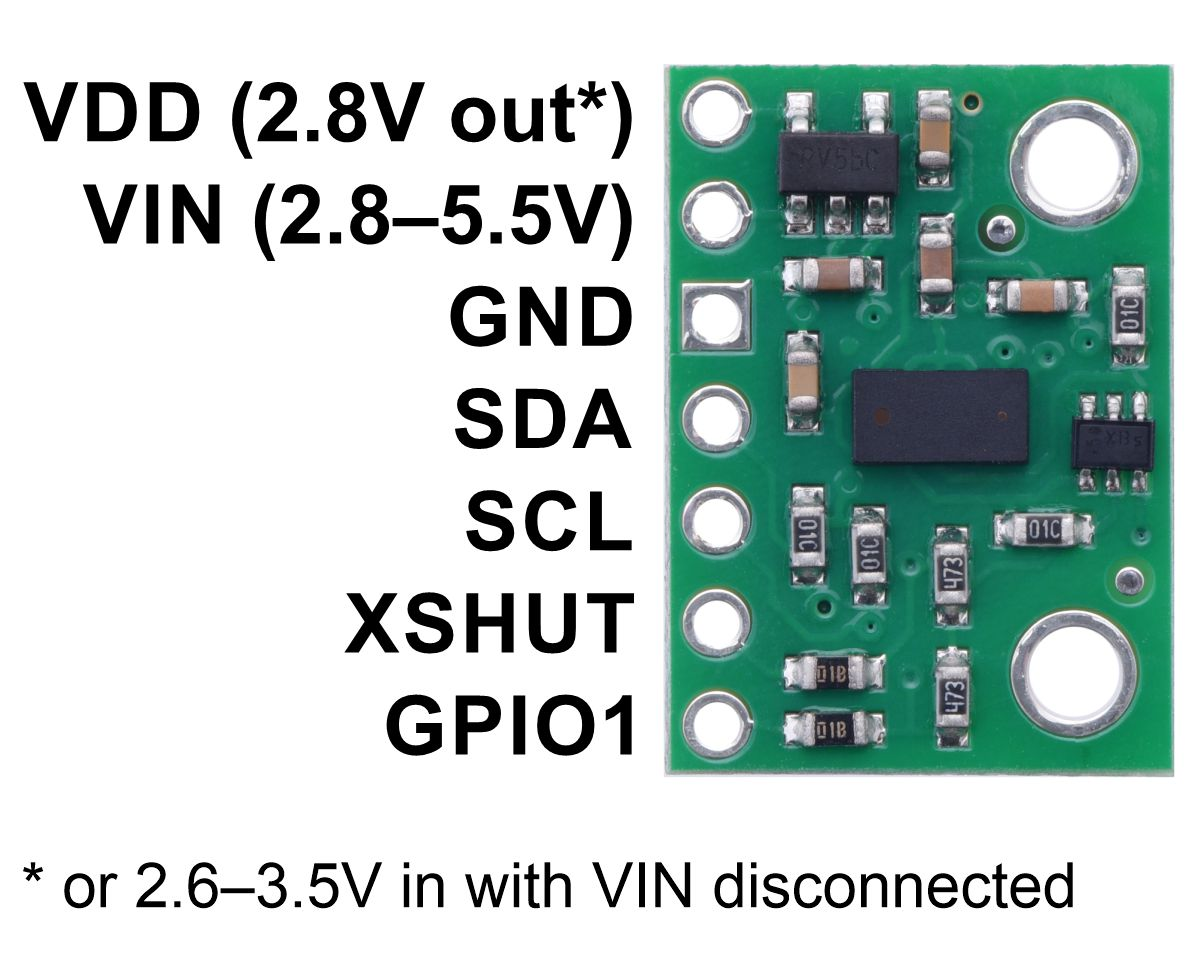
\includegraphics[width=\textwidth]{figures/02_hardware/vl53l1x_modulo_pololu_configurazione_pin.jpg}
			\caption{Pin Configuration}
			\label{fig:img1}
		\end{minipage}
		\hfill
		\begin{minipage}{0.45\textwidth}
			\centering
			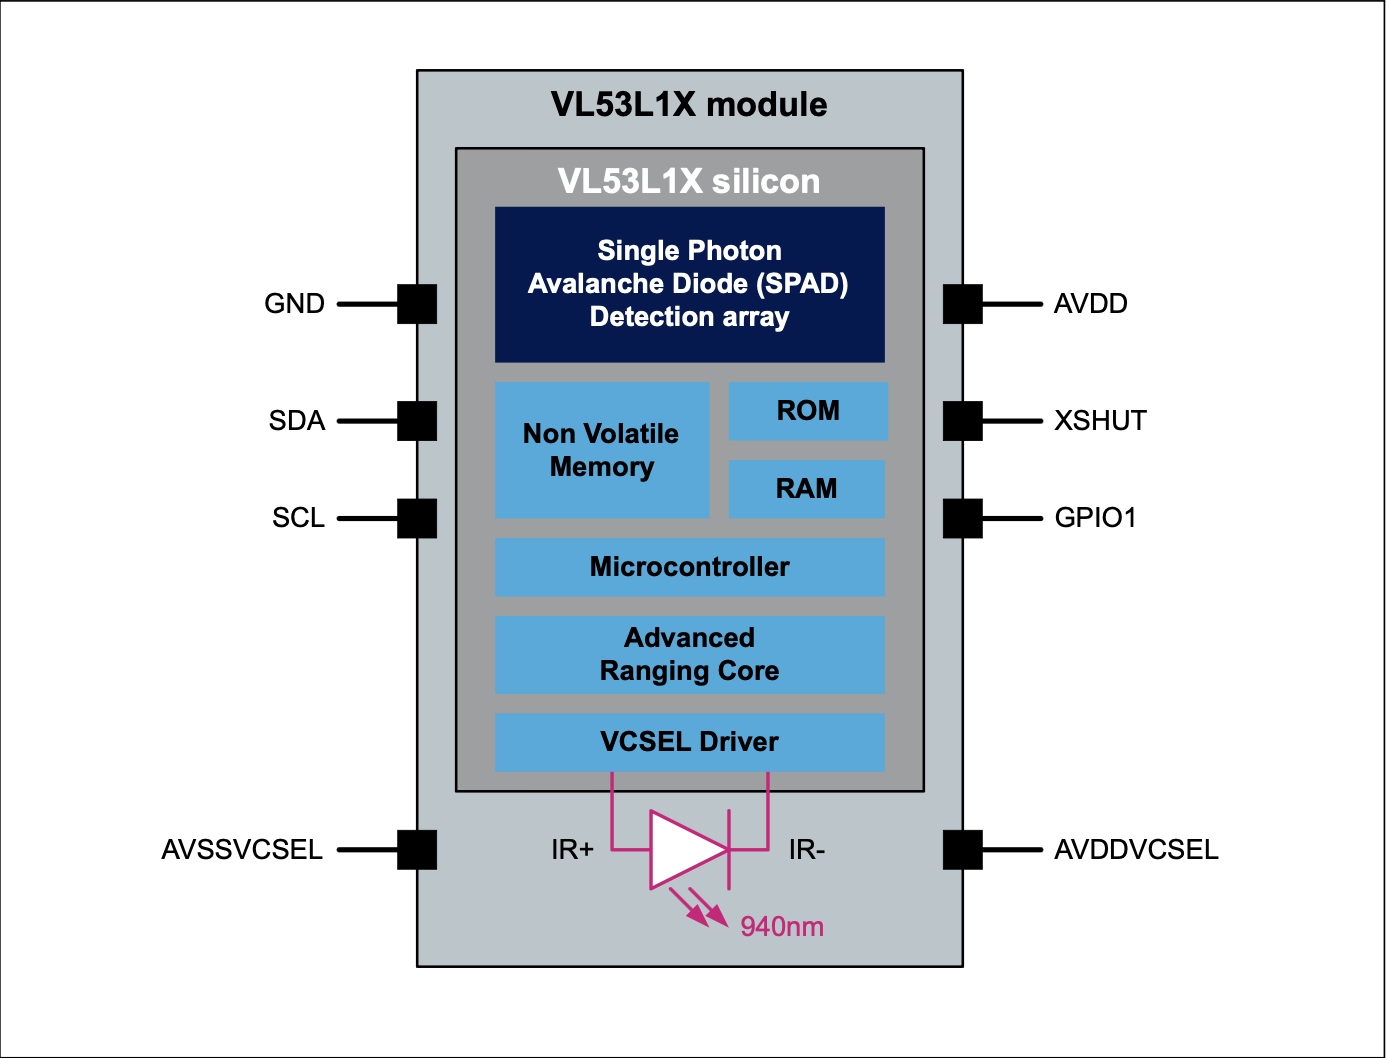
\includegraphics[width=\textwidth]{figures/02_hardware/vl53l1x_schema_blocchi_sistema.png}
			\caption{System Block Diagram}
			\label{fig:img2}
		\end{minipage}
		\
		{\footnotesize L'immagine a sinistra specifica la disposizione della piedinatura del modulo \textit{Pololu} (\textit{P.C.: Pin Configuration}), mentre la figura di destra rappresenta la suddivisione modulare del \textit{VL53L1X} (\textit{S.B.D.: System Block Diagram}).}
	\end{figure}
	\paragraph{\small{Emettitore}}\mbox{}\\
	Il \textit{VL53L1X} integra un emettitore \textbf{laser a infrarossi con lunghezza d'onda pari a 940 [nm]}, classificato come \textbf{\textit{Classe 1}} secondo la norma internazionale \textbf{IEC 60825-1}.
	Tale classificazione descrive il livello di rischio associato all'esposizione umana alla radiazione laser, in particolare per occhi e pelle. La norma suddivide infatti gli emettitori in diverse \textit{classi}, ciascuna associata a un diverso livello di pericolosità. Nel caso di un laser di \textit{Classe 1}, come quello utilizzato dal dispositivo, le condizioni operative normali sono considerate sicure per l'esposizione di occhi e pelle.
	
	\begin{figure}[H]
		\centering
		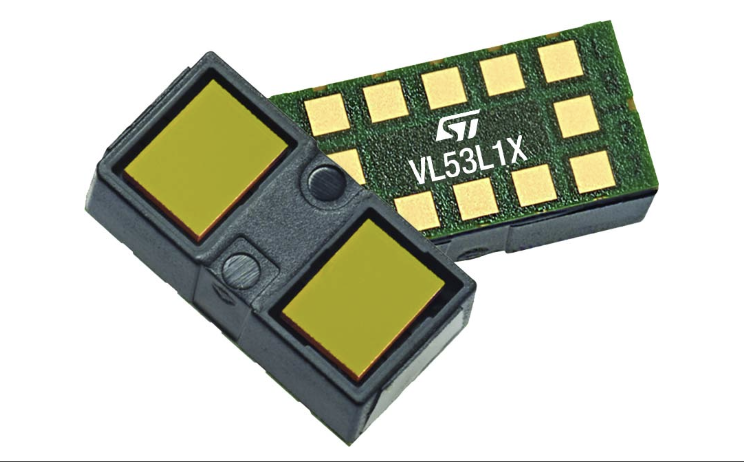
\includegraphics[width=0.6\textwidth]{figures/02_hardware/vl53l1x_dettaglio_emettitore.png}
		\caption{VL53L1X, dettaglio sull'emettitore}
	\end{figure}
	
	\paragraph{\small{Field of View  (FoV)}}\mbox{}\\
	Il \textit{Field of View} rappresenta l'angolo massimo entro il quale il dispositivo è in grado di rilevare un oggetto. Per il sensore in esame, il \textbf{FoV} è pari a circa \textbf{27\degree}.\\
	A seguire, un'immagine esplicativa del \textit{FoV}:
	\begin{figure}[H]
		\centering
		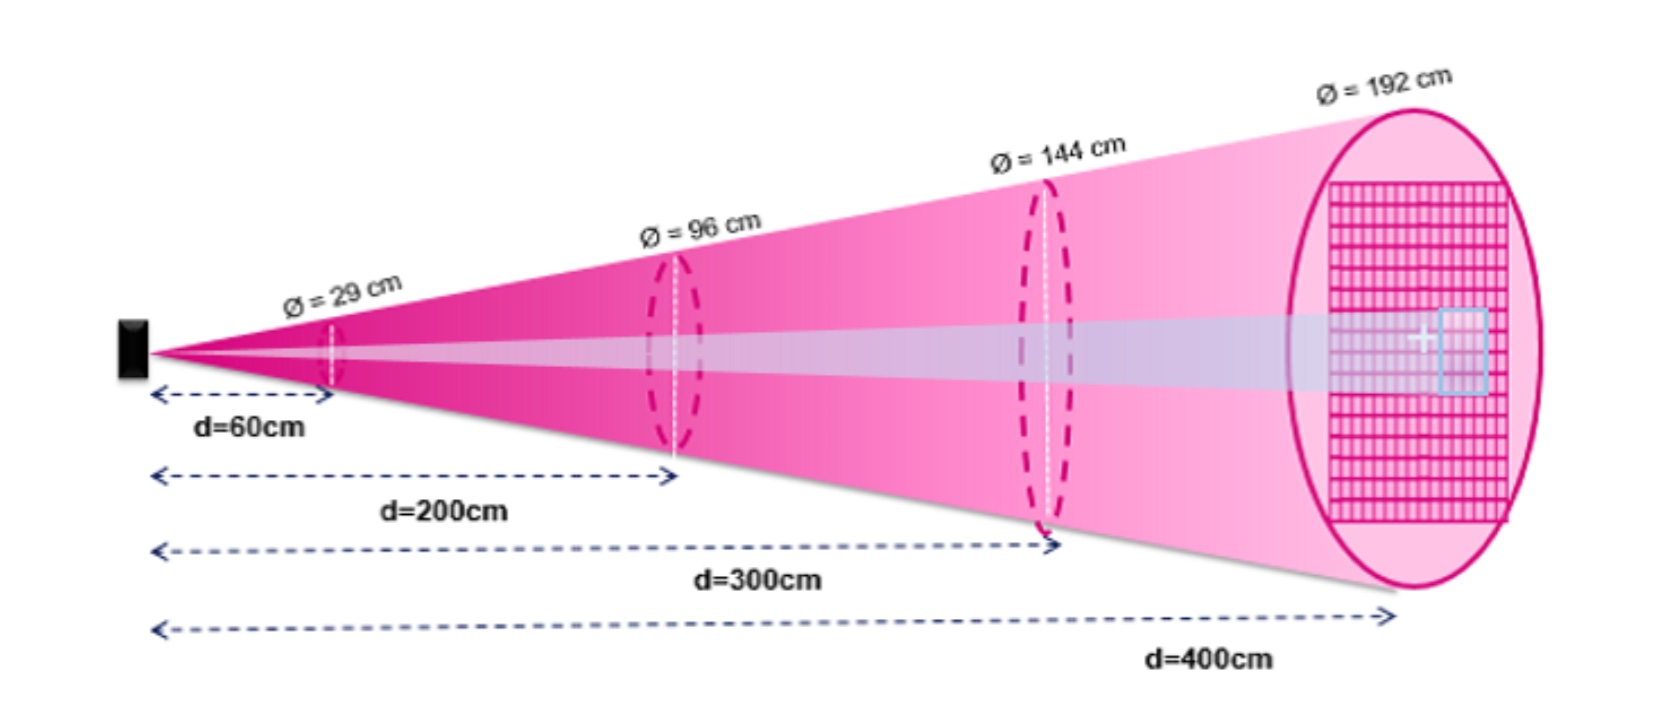
\includegraphics[width=0.7\textwidth]{figures/02_hardware/vl53l1x_cono_campo_visivo.jpg}
		\caption{Field of View del VL53L1X}
	\end{figure}
	
	\paragraph{\small{Region-of-interest (R.O.I)}}\mbox{}\\
	Con \textit{Region-Of-Interest} si indica una funzione del \textit{VL53L1X} che permette di restringere il \textit{Field of View} effettivamente utilizzato durante la misura.
	Questa opzione è utile quando si vuole migliorare la precisione su oggetti di piccole dimensioni.\\
	Nel presente progetto, il sensore è impiegato per la misura dell'altitudine del \textit{DPDF}; di conseguenza, la funzione \textit{R.O.I.} non è mai stata utilizzata e il \textit{FoV} è stato lasciato al valore nominale di 27\degree.
	
	\paragraph{\small{Prestazioni di misura, Timing Budget e modalità operative di misura}}\mbox{}\\
	Il \textit{VL53L1X} offre buone prestazioni di misura in termini di accuratezza e rapidità. Il dispositivo è in grado di misurare distanze fino a 4 [m], con frequenze che possono arrivare fino a 50 [Hz].
	Per adattarsi a scenari applicativi differenti, il sensore consente di selezionare la modalità di misura più adatta, bilanciando portata, robustezza e velocità di acquisizione.
	A seguire, una tabella riassuntiva delle modalità di misura offerte dal dispositivo:
	\begin{table}[htb]
		\centering
		\caption{VL53L1X. Modalità di misura}
		\resizebox{\textwidth}{!}{
			\begin{tabular}{l c c}
				\toprule
				\textit{Modalità} & Range massimo in condizioni di scarsa luce (approssimato) & Range massimo con luce ambientale \\
				\midrule
				\textit{Short}    & 136 [cm]                                                  & 135 [cm]                          \\
				\textit{Medium}   & 290 [cm]                                                  & 76 [cm]                           \\
				\textit{Long}     & 360 [cm]                                                  & 73 [cm]                           \\
				\bottomrule
			\end{tabular}
		}
		\label{tab:VL53L1X. Hardware}
	\end{table}
	\begin{center}
		\footnotesize \textit{Tabella riportata dal datasheet ufficiale del VL53L1X. I valori presentati, sono stati ricavati sotto le seguenti condizioni : \textit{timing budget} = 100 [ms], bersaglio bianco, riflettanza : 88\%, luce ambientale : 200 [kcps/SPAD].}
	\end{center}
	
	La \textit{Short ranging mode} è pensata per misure ravvicinate, stabili e robuste anche in ambienti luminosi. La \textit{Long range mode} privilegia invece la massima portata, accettando però misure più sensibili al rumore. Tra queste due opzioni si colloca la \textit{Medium range mode}, che rappresenta un compromesso tra distanza operativa e robustezza.\\
	L'ambiente in cui sono stati eseguiti i test di volo era fortemente illuminato; inoltre, i fili di sostegno costituivano un vincolo sull'altitudine massima raggiungibile, che non superava i 60 [cm].\\
	Per queste ragioni, ai fini progettuali è stata scelta la \textbf{\textit{Short ranging mode}}, che è rimasta l'unica modalità operativa utilizzata per l'intero progetto.\\
	Per gestire in modo accurato il compromesso tra temporizzazione e precisione, è stata sfruttata la funzione di \textbf{Timing Budget} del sensore. Con \textit{Timing Budget} si indica il tempo totale impiegato dal sensore per eseguire una singola misura di distanza. Tale grandezza è espressa in [ms] e può assumere valori compresi nell'intervallo \textbf{[20$\div$1000] [ms]}.
	Un aumento del \textit{Timing Budget} comporta una riduzione della frequenza di misura ma, al tempo stesso, ne migliora l'accuratezza e la stabilità.\\
	La documentazione suggerisce che un \textit{Timing Budget} di \textbf{33 ms} offra un buon compromesso tra velocità e accuratezza; per questo motivo, ai fini progettuali, è stato selezionato tale valore. La gestione dell'effettiva temporizzazione è stata poi completata intervenendo sull'\textit{Inter-Measurement Period}, approfondito nella sezione \textit{Software}.\\
	A seguire, un'immagine riportata direttamente dallo \textit{User Manual} del \textit{VL53L1X}, raffigurante le prestazioni di misura a fronte di diversi valori del \textit{Timing Budget}.
	\begin{figure}[ht]
		\centering
		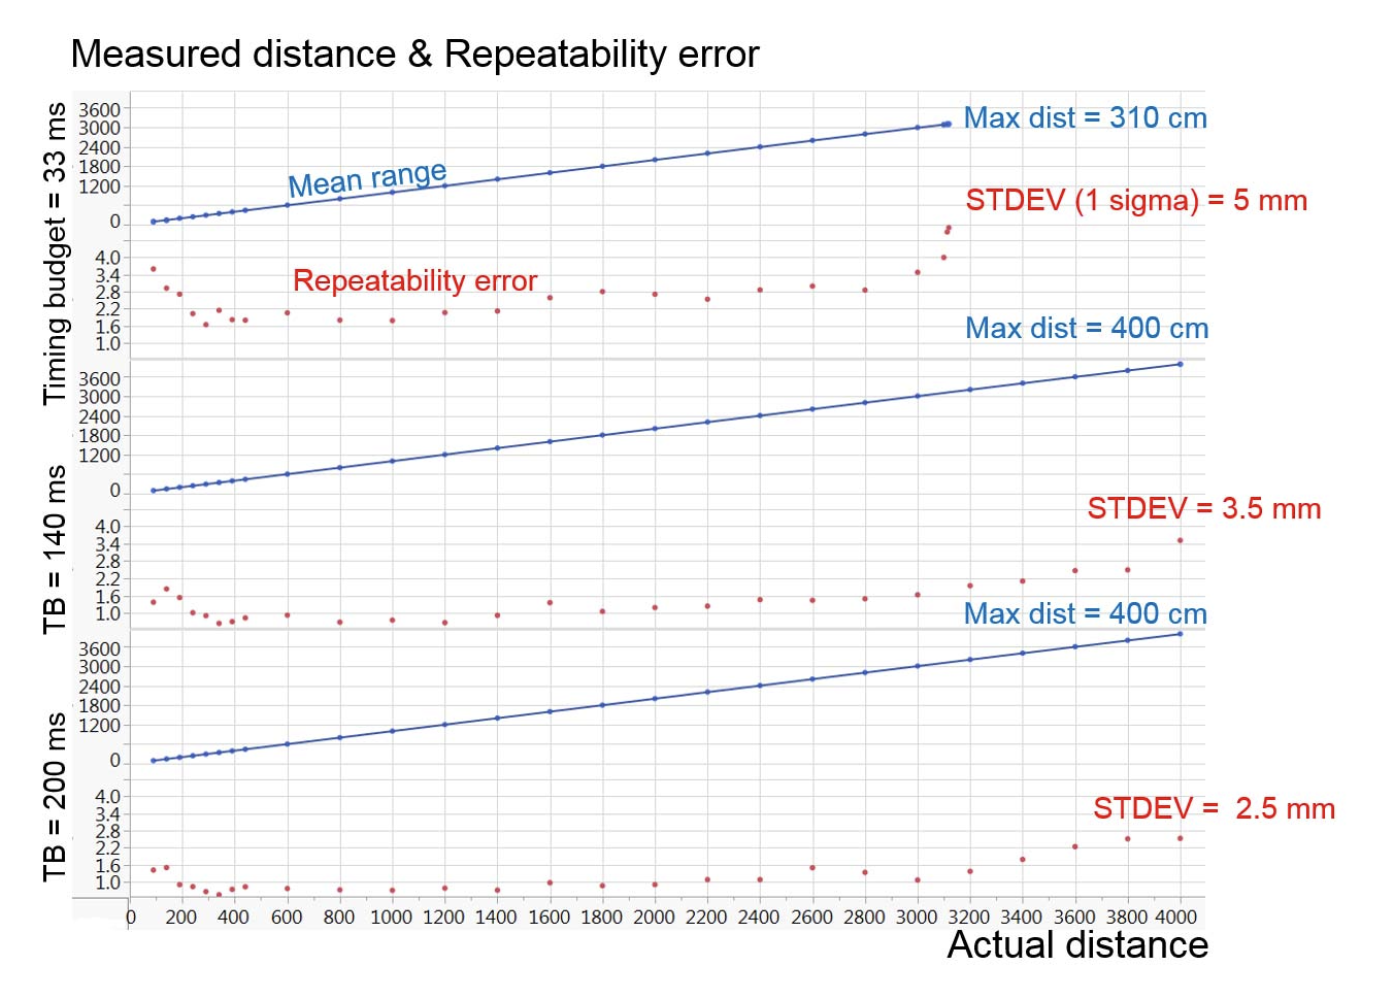
\includegraphics[width=0.7\textwidth]{figures/02_hardware/vl53l1x_prestazioni_timing_budget.png}
		\caption{VL53L1X, prestazioni di misura}
	\end{figure}
	
	\section{Schema dei collegamenti}

	\begin{figure}[H]
		\centering
		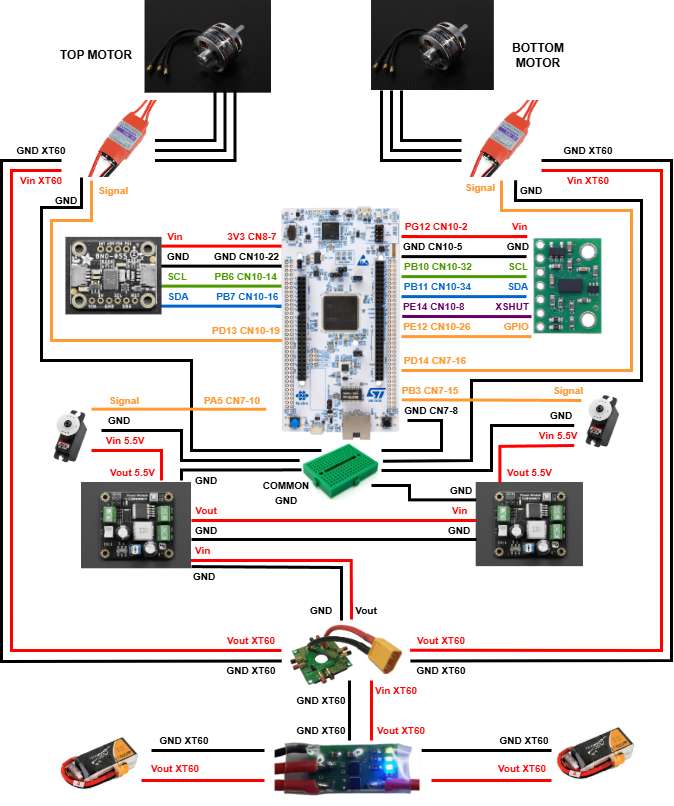
\includegraphics[width=0.8\textwidth,keepaspectratio]{figures/02_hardware/schema_collegamenti_ducted_fan.png}
		\caption{Schema dei collegamenti}
		\label{fig:schema}
	\end{figure}

	\subsection{Tabelle dei collegamenti}
	Di seguito sono riportati i collegamenti elettrici tra i principali componenti del sistema e la scheda di controllo.

	\paragraph{Collegamenti NUCLEO-H745ZI-Q e VL53L1X}\mbox{}\\
	Il sensore \textit{VL53L1X} (STMicroelectronics) è stato collegato direttamente alla \textit{NUCLEO-H745ZI-Q}.
	\begin{table}[H]
		\centering
		\begin{tabular}{l l}
			\toprule
			\textbf{VL53L1X} & \textbf{NUCLEO-H745ZI-Q} \\
			\midrule
			Vin & PG12, CN10-2 \\
			GND & GND, CN10-5 \\
			SCL & SCL I2C2: PB10, CN10-32 \\
			SDA & SDA I2C2: PB11, CN10-34 \\
			XSHUT & PE14, CN10-8 \\
			GPIO & CN10-26 \\
			\bottomrule
		\end{tabular}
		\caption{Collegamenti NUCLEO-H745ZI-Q e VL53L1X}
	\end{table}

	\paragraph{Collegamenti NUCLEO-H745ZI-Q e BNO055}\mbox{}\\
	Il sensore \textit{BNO055} (Bosch Sensortec) è stato collegato direttamente alla \textit{NUCLEO-H745ZI-Q}.
	\begin{table}[H]
		\centering
		\begin{tabular}{l l}
			\toprule
			\textbf{BNO055} & \textbf{NUCLEO-H745ZI-Q} \\
			\midrule
			Vin & 3.3V, CN8-7 \\
			GND & GND, CN8-11 \\
			SCL & SCL I2C1: PB6, CN10-14 \\
			SDA & SDA I2C1: PB7, CN10-16 \\
			\bottomrule
		\end{tabular}
		\caption{Collegamenti NUCLEO-H745ZI-Q e BNO055}
	\end{table}

	\paragraph{Collegamenti DF-Robot, servo e NUCLEO-H745ZI-Q}\mbox{}\\
	Per garantire il corretto funzionamento del comparto servomotori è necessario un riferimento di massa comune. Nel progetto è stata utilizzata una \textit{breadboard} esterna per distribuire la massa proveniente dalla NUCLEO-H745ZI-Q (GND, CN7-8). L'alimentazione dei servomotori è stata prelevata direttamente dall'uscita dei convertitori di tensione collegati in serie.

	\begin{table}[H]
		\centering
		\begin{tabular}{l l l l}
			\toprule
			\textbf{DF-Robot roll} & \textbf{Roll-servo} & \textbf{Common GND} & \textbf{NUCLEO-H745ZI-Q} \\
			\midrule
			Vout-3 & Vin (5.5V) & - & - \\
			Vout-GND & GND & C.GND & GND, CN7-8 \\
			- & Signal & - & TIM2-CH1: PA5, CN7-10 \\
			\bottomrule
		\end{tabular}
		\caption{Collegamenti NUCLEO-H745ZI-Q e Roll-servo}
	\end{table}

	\begin{table}[H]
		\centering
		\begin{tabular}{l l l l}
			\toprule
			\textbf{DF-Robot pitch} & \textbf{Pitch-servo} & \textbf{Common GND} & \textbf{NUCLEO-H745ZI-Q} \\
			\midrule
			Vout-3 & Vin (5.5V) & - & - \\
			Vout-GND & GND & C.GND & GND, CN7-8 \\
			- & Signal & - & TIM2-CH2: PB3, CN7-15 \\
			\bottomrule
		\end{tabular}
		\caption{Collegamenti NUCLEO-H745ZI-Q e Pitch-servo}
	\end{table}

	\paragraph{Collegamenti Power Distribution Module, ESC e NUCLEO-H745ZI-Q}\mbox{}\\
	Per il comparto motori, gli ESC sono collegati al \textit{Power Distribution Module}, a sua volta connesso al comparto batterie-PSM e ai motori tramite i rispettivi connettori trifase. Il terminale di massa degli ESC deve condividere la massa della NUCLEO-H745ZI-Q, mentre il terminale \textit{Signal} deve essere connesso al pin PWM della scheda.

	\begin{table}[H]
		\centering
		\begin{tabular}{l l l}
			\toprule
			\textbf{Power Distribution Module} & \textbf{Top-motor-ESC} & \textbf{NUCLEO-H745ZI-Q} \\
			\midrule
			Vout XT-60 & Vin XT-60 & - \\
			GND XT-60 & GND XT-60 & - \\
			- & Signal & TIM4-CH2: PD13, CN10-19 \\
			- & GND & GND \\
			\bottomrule
		\end{tabular}
		\caption{Collegamenti NUCLEO-H745ZI-Q e Top-motor-ESC}
	\end{table}

	\begin{table}[H]
		\centering
		\begin{tabular}{l l l}
			\toprule
			\textbf{Power Distribution Module} & \textbf{Bottom-motor-ESC} & \textbf{NUCLEO-H745ZI-Q} \\
			\midrule
			Vout XT-60 & Vin XT-60 & - \\
			GND XT-60 & GND XT-60 & - \\
			- & Signal & TIM4-CH3: PD14, CN7-16 \\
			- & GND & GND \\
			\bottomrule
		\end{tabular}
		\caption{Collegamenti NUCLEO-H745ZI-Q e Bottom-motor-ESC}
	\end{table}

	\textit{Nota}: il dispositivo che riceve il segnale PWM deve condividere lo stesso riferimento di massa del dispositivo che genera tale segnale.

	\chapter{Software}
	Il firmware di controllo del \textit{Double Propeller Ducted-Fan (DPDF)} è stato sviluppato con l'obiettivo di ottenere una condizione di \textit{hovering} sufficientemente stabile del velivolo.
	L'implementazione è stata realizzata in linguaggio C all'interno di \textit{STM32CubeIDE} (versione \textbf{1.16.1}), utilizzando i flussi di configurazione hardware, generazione codice basata su HAL (\textit{Hardware Abstraction Layer}), compilazione e debug integrati nell'ambiente.
	Per la configurazione delle periferiche del microcontrollore \textit{STM32H745ZI-TQ6} è stato impiegato \textit{STM32CubeMX} (versione \textbf{6.12.1}).
	
	Per i sensori \textit{BNO055} (Bosch Sensortec) e \textit{VL53L1X} (STMicroelectronics) sono stati integrati i driver ufficiali dei produttori, nativamente \textit{platform-agnostic}, e adattati al contesto HAL tramite un sottile livello di interfaccia per comunicazione, interrupt e gestione dei pin.
	Una parte del sub-firmware di base, in particolare l'infrastruttura iniziale e alcuni moduli driver, era già stata sviluppata in precedenza. Il lavoro svolto si è quindi concentrato sulla modifica, miglioramento, integrazione e validazione del codice nel contesto del progetto DPDF.
	
	Nelle sezioni successive vengono quindi descritti i diagrammi di flusso e l'organizzazione del firmware adottata nel progetto, mantenendo la terminologia operativa usata nel codice (i termini \textit{procedura} e \textit{funzione} sono considerati equivalenti in questa relazione).
	
	\section{Diagrammi di flusso}
	Nella presente sezione sono stati riportati i diagrammi di flusso esplicativi del funzionamento del \textit{firmware}. Poiché i driver di gestione del \textit{VL53L1X} e \textit{BNO055} sono esterni allo sviluppo, sono stati riportati anche i diagrammi di flusso di questi, in tal modo da specificare la procedura di estrazione dell'informazione.
	
	\subsection{Diagramma di flusso del firmware}
	\begin{figure}[H]
		\centering
		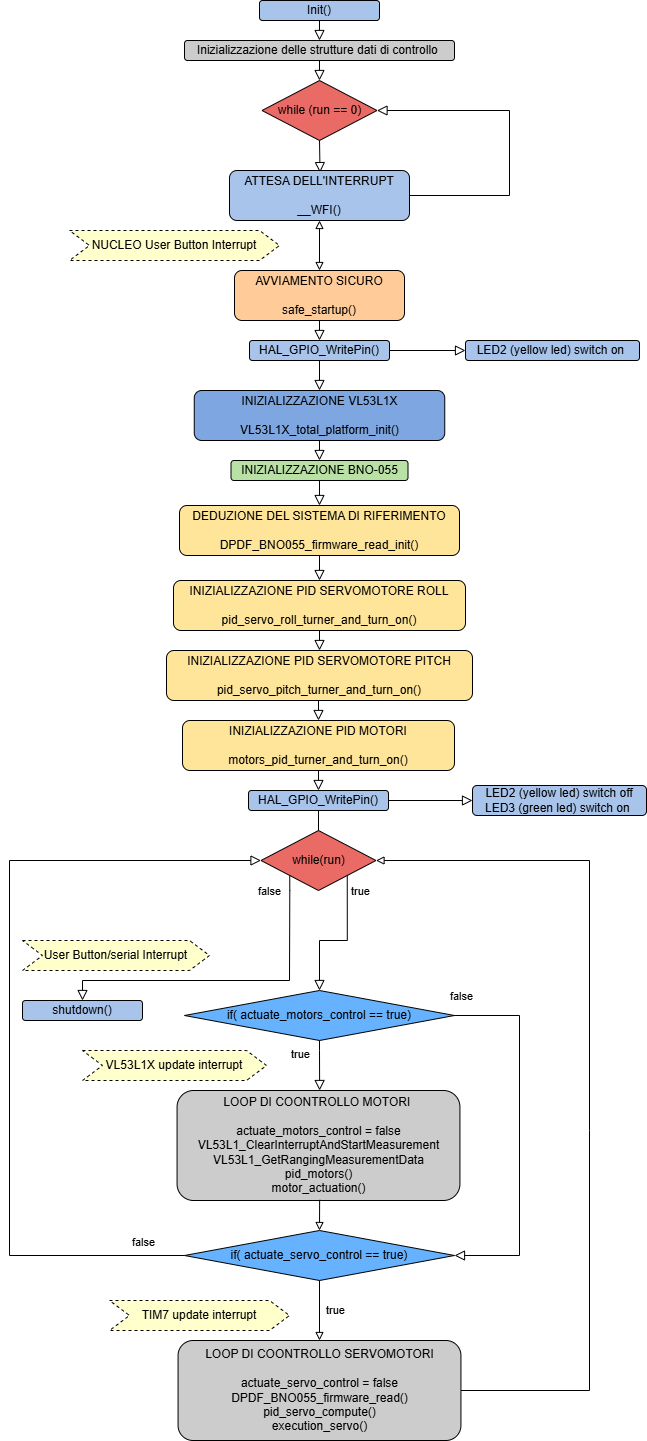
\includegraphics[width=0.55\textwidth,keepaspectratio]{figures/03_software/diagramma_di_flusso_generale.png}
		\caption{Diagramma di flusso del funzionamento del firmware}
		\label{fig:diagramma-firmware-generale}
	\end{figure}
	

	\subsection{Diagramma di flusso del VL53L1X per misurazione di quota}
	
	\begin{figure}[H]
		\centering
		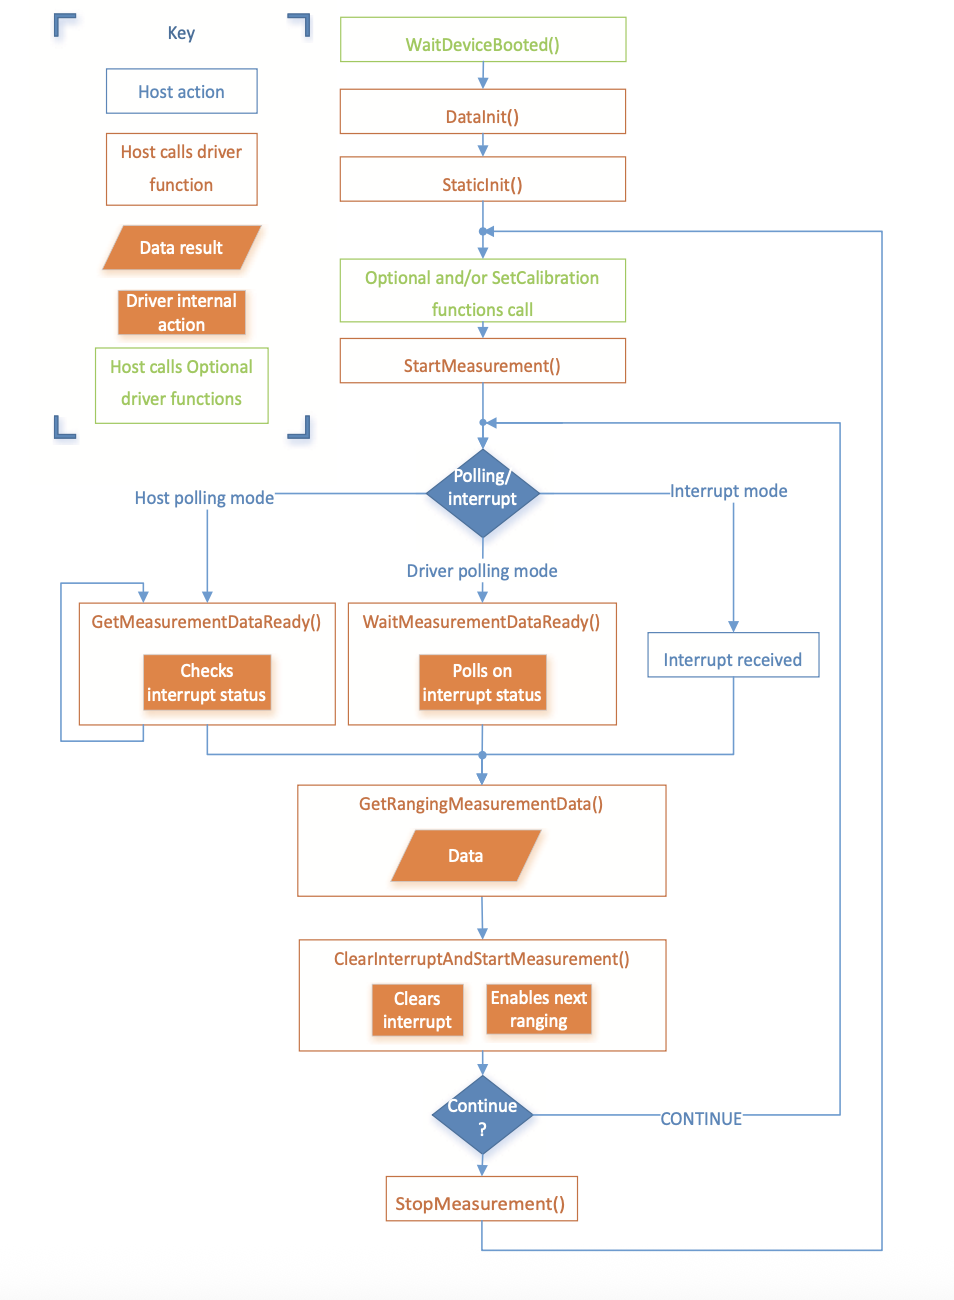
\includegraphics[width=0.88\textwidth,keepaspectratio]{figures/03_software/diagramma_di_flusso_VL53L1X.png}
		\caption{Diagramma di flusso del VL53L1X per la misurazione della quota}
		\label{fig:diagramma-vl53l1x}
	\end{figure}
	
	\subsection{Diagramma di flusso del BNO055}
	
	\begin{figure}[H]
		\centering
		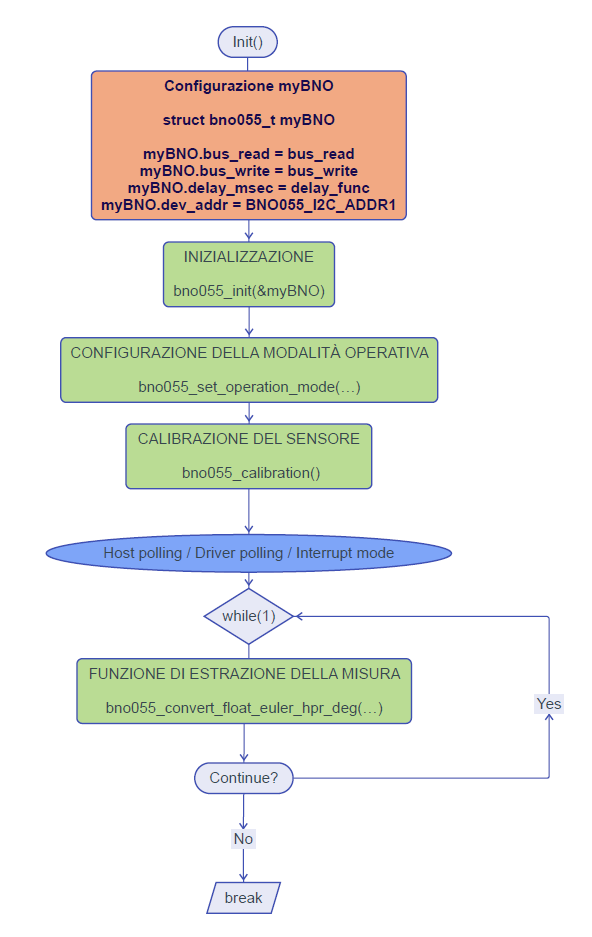
\includegraphics[height=0.78\textheight,keepaspectratio]{figures/03_software/diagramma_di_flusso_BNO055.png}
		\caption{Diagramma di flusso del BNO055 per l'estrazione dell'orientamento}
		\label{fig:diagramma-bno055}
	\end{figure}
	
	\section{Gestione singoli componenti}
	Il firmware è organizzato in modo modulare perché, in un sistema di controllo reale, la chiarezza dell'architettura ha un impatto diretto sulla robustezza. Il file \texttt{main.c} svolge il ruolo di supervisore: inizializza le periferiche, imposta i riferimenti, configura i controllori e coordina il ciclo principale. I moduli specialistici separano invece le responsabilità fisiche: \texttt{pwm.c} traduce i comandi in segnali per motori e servo, \texttt{pid.c} implementa il nucleo numerico dei regolatori e il filtro mediano, \texttt{tof.c} corregge la misura di quota rispetto all'inclinazione del velivolo, mentre \texttt{imu.c} raccoglie lettura e riorientamento delle misure di assetto.

	Questa suddivisione non è utile soltanto per ``tenere ordinato'' il codice. Il motivo principale è che i blocchi time-critical possono restare semplici, mentre la logica numerica viene mantenuta nel ciclo principale. Le callback di interrupt non eseguono perciò elaborazioni di controllo, ma si limitano a notificare la presenza di un evento tramite le flag \texttt{actuate\_motors\_control} e \texttt{actuate\allowbreak\_servo\allowbreak\_control}. Così si riduce il tempo passato in ISR, si limita il jitter e si rende il percorso misura-elaborazione-comando più leggibile e verificabile.

	\subsection{Architettura del controllo}
	L'architettura prevista è costruita come un sistema a due rami principali, ciascuno dedicato a una grandezza fisica ben definita. Il primo ramo controlla la quota, cioè la distanza verticale dal piano di riferimento. Il secondo controlla l'assetto, cioè la vicinanza degli angoli di \textit{roll} e \textit{pitch} al valore nullo. Separare i due rami è una scelta naturale perché la quota dipende in modo predominante dalla spinta totale, mentre l'assetto dipende soprattutto dai momenti aerodinamici generati dai flap.

	Dal punto di vista concettuale, il controllo opera secondo la seguente catena causale: il sensore misura una grandezza fisica, la misura viene trasformata nella coordinata utile al problema, il regolatore confronta il valore misurato con il riferimento e genera un comando che abbia lo stesso significato fisico dell'attuatore. Nel ramo motori, l'uscita del controllore è un livello di comando PWM comune ai due ESC; nel ramo flap, l'uscita del controllore è invece un angolo richiesto, successivamente convertito in PWM per i servo. Questo passaggio intermedio è importante perché evita di confondere il livello di controllo con il livello di attuazione.

	La scomposizione adottata può essere riassunta come segue:
	\begin{itemize}
		\item \textbf{quota}: riferimento verticale $z_{ref}$, misura proveniente dal VL53L1X, comando comune ai due motori;
		\item \textbf{assetto}: riferimenti $\phi_{ref}=0$ e $\theta_{ref}=0$, misura proveniente dal BNO055, comando angolare ai flap di \textit{roll} e \textit{pitch}.
	\end{itemize}
	La presenza di due motori controrotanti e di due flap ortogonali rende infatti possibile associare in maniera sufficientemente pulita ciascun attuatore alla grandezza dominante che deve correggere.

	\subsection{Definizione delle costanti e delle strutture condivise}
	Il file \texttt{DPDF\_var\_def.h} raccoglie i parametri numerici che descrivono il comportamento ammissibile del sistema. Centralizzare questi valori non serve soltanto a evitare la dispersione di costanti nel codice, ma soprattutto a rendere esplicito il confine tra legge di controllo e limiti imposti dall'hardware reale. In un problema di controllo embedded, infatti, il regolatore ideale e l'attuatore fisico non coincidono: il primo potrebbe richiedere qualunque valore, mentre il secondo può operare solo entro un intervallo ristretto e sicuro.

	Le macro principali sono le seguenti:
	\begin{itemize}
		\item \texttt{NUMBER\_OF\_TOGGLES} fissa la durata del conto alla rovescia prima dell'avvio;
		\item \texttt{UPPER\_LIMIT\_MOTOR} e \texttt{LOWER\_LIMIT\_MOTOR} delimitano il range PWM utilizzabile dagli ESC;
		\item \texttt{UPPER\_LIMIT\_SERVO}, \texttt{CENTER\_SERVO} e \texttt{LOWER\_LIMIT\_SERVO} definiscono la zona di lavoro meccanicamente sicura dei servomotori;
		\item \texttt{CCR\_PER\_DEGREE} e \texttt{MAX\_FLAP\_ANGLE\_DEG} descrivono la conversione tra grandezza fisica richiesta al flap e valore effettivamente scrivibile nel registro timer.
	\end{itemize}

	Il significato di queste costanti è quindi progettuale prima ancora che implementativo. La saturazione dei motori impedisce di uscire dal range accettato dagli ESC; quella dei servo evita il raggiungimento di fine corsa inutili o dannosi. Dichiarare questi limiti in modo esplicito rende il controllore più interpretabile, perché ogni uscita numerica può essere letta come ``comando valido e realizzabile'', non come semplice risultato di una formula.

	Il firmware utilizza inoltre una struttura PID unica, inizializzata tramite \texttt{pid\_init()} e aggiornata tramite \texttt{pid\_compute()}. Questa scelta uniforma il comportamento interno dei tre regolatori: inizializzazione dello stato, gestione dell'integrale, calcolo della derivata e saturazione seguono la stessa logica, mentre cambiano i parametri che descrivono il problema fisico. In questo modo il codice non contiene tre implementazioni diverse dello stesso concetto, ma un solo strumento generale specializzato tramite configurazione.

	\begin{lstlisting}[style=base,language=C,caption={Costanti principali usate dal firmware per definire i limiti hardware e di sicurezza}]
		#define UPPER_LIMIT_MOTOR                      1500
		#define LOWER_LIMIT_MOTOR                       750
		#define UPPER_LIMIT_SERVO                      1545
		#define CENTER_SERVO                           1125
		#define LOWER_LIMIT_SERVO                       705
		#define CCR_PER_DEGREE                          5.0f
		#define MAX_FLAP_ANGLE_DEG                     60.0f
	\end{lstlisting}

	\subsection{Teoria del regolatore PID}
	Il regolatore PID nasce dall'idea di trasformare l'errore di controllo in un comando che tenga conto non soltanto della sua ampiezza istantanea, ma anche della sua storia e della sua tendenza futura. Indicando con $r(t)$ il riferimento, con $y(t)$ la variabile misurata e con
	\begin{equation}
		e(t)=r(t)-y(t)
	\end{equation}
	l'errore di controllo, la forma continua classica del PID è
	\begin{equation}
		u(t)=K_p e(t) + K_i \int_0^t e(\tau)\,d\tau + K_d\frac{de(t)}{dt}.
	\end{equation}
	Questa scrittura è utile perché separa tre effetti fisicamente diversi. Il termine proporzionale reagisce subito all'errore presente e determina la prontezza della risposta. Il termine integrale accumula l'errore nel tempo e serve a rimuovere gli scostamenti persistenti, cioè quelle condizioni in cui il sistema resta vicino al riferimento ma non vi converge esattamente. Il termine derivativo, infine, reagisce alla rapidità con cui l'errore cambia e introduce un effetto di anticipazione che tende a smorzare la dinamica.

	Dal punto di vista ingegneristico, il PID non è interessante perché somma tre termini, ma perché consente di assegnare un significato fisico distinto a ciascuna componente dell'azione di controllo. In un sistema come il DPDF questo è particolarmente utile: una parte del comando deve reagire rapidamente agli scostamenti, una parte può compensare errori sistematici e una parte, se necessaria, può limitare l'insorgenza di oscillazioni.

	Una forma equivalente, spesso utile nella taratura, si ottiene introducendo il tempo integrale $T_i$ e il tempo derivativo $T_d$:
	\begin{equation}
		u(t)=K_p\left[e(t)+\frac{1}{T_i}\int_0^t e(\tau)\,d\tau + T_d\frac{de(t)}{dt}\right].
	\end{equation}
	Questa parametrizzazione mette in evidenza che il guadagno proporzionale fissa la scala complessiva dell'azione di controllo, mentre integrale e derivata modellano il modo in cui il regolatore reagisce alla persistenza e alla variazione dell'errore.

	\subsection{PID discreto adottato nel firmware}
	Il firmware non implementa un PID continuo ideale, ma una sua approssimazione numerica causale, compatibile con il periodo di campionamento, con il rumore dei sensori e con i limiti fisici degli attuatori. In altre parole, il passaggio al discreto non è una semplice riscrittura formale: è il modo con cui la legge di controllo viene resa eseguibile da un microcontrollore che riceve misure a istanti separati e aggiorna il comando solo quando dispone di nuovi dati.

	Indicando con $k$ l'indice temporale e con $T_s$ il periodo di campionamento, si definisce innanzitutto
	\begin{equation}
		e[k]=r[k]-y[k].
	\end{equation}
	La forma concettuale implementata nel firmware è
	\begin{equation}
		u[k]=u_0 + P[k] + I[k] + D[k],
	\end{equation}
	dove $u_0$ è un eventuale offset, mentre i tre contributi sono calcolati come
	\begin{align}
		P[k] &= K_p e[k], \\
		I[k] &= I[k-1] + K_i T_s e[k], \\
		D_e[k] &= \frac{K_d}{T_s}\bigl(e[k]-e[k-1]\bigr).
	\end{align}
	La seconda equazione è la discretizzazione in avanti dell'integrale e mostra con chiarezza il motivo per cui il termine integrale può diventare dominante: se l'errore persiste, il suo contributo si accumula passo dopo passo. È proprio questa capacità di memoria che rende l'integrale utile contro gli errori statici, ma anche potenzialmente pericoloso se non viene limitato.

	Nel firmware il termine derivativo può essere calcolato anche sulla misura, scelta particolarmente utile quando il riferimento può cambiare nel corso delle prove e non si vuole che un suo gradino produca un picco artificiale di comando. In tal caso la forma adottata è
	\begin{equation}
		D_y[k]= -\frac{K_d}{T_s}\bigl(y[k]-y[k-1]\bigr).
	\end{equation}
	Il segno meno compare perché, se la misura cresce a parità di riferimento, l'errore diminuisce. Dal punto di vista fisico, derivare la misura significa far reagire il regolatore al moto osservato del sistema più che al cambiamento imposto dall'esterno al riferimento.

	Il comando grezzo viene quindi scritto come
	\begin{equation}
		u_{raw}[k]=u_0 + K_p e[k] + I[k] + D[k].
	\end{equation}
	Questa è la quantità che il PID vorrebbe applicare in assenza di vincoli. In un sistema reale, tuttavia, il comando non può essere arbitrario: motori e servomotori lavorano entro intervalli ben precisi. Per questa ragione si introduce la saturazione logica del controllore
	\begin{equation}
		u_{pid}[k]=\mathrm{clamp}\bigl(u_{raw}[k],u_{min},u_{max}\bigr),
	\end{equation}
	che ha il compito di rendere l'uscita del regolatore compatibile con il dominio di lavoro previsto. A questa si sovrappone poi una seconda limitazione, di natura strettamente hardware, applicata nella fase di attuazione: per i motori il PWM deve restare nel range accettato dagli ESC, mentre per i servo il comando deve rispettare sia il campo angolare sicuro sia la corrispondente finestra di conteggi timer. Distinguere questi due livelli è utile perché il primo appartiene alla legge di controllo, mentre il secondo appartiene all'interfaccia fisica con l'attuatore.

	\subsection{Scelta dei tempi di campionamento}
	I due rami di controllo non sono campionati alla stessa frequenza perché non osservano la stessa dinamica né usano la stessa sorgente di misura. Il ramo servo lavora con periodo nominale di \texttt{10 ms}, generato da \texttt{TIM7}, perché il controllo di assetto deve reagire con maggiore rapidità alle variazioni angolari. Il ramo motori lavora invece con periodo nominale di circa \texttt{33 ms}, associato alla disponibilità di nuove misure del VL53L1X, perché la dinamica della quota è più lenta e la misura ToF ha tempi caratteristici differenti.

	Questa scelta evita due errori opposti. Campionare troppo lentamente l'assetto renderebbe il sistema poco reattivo; campionare inutilmente troppo in fretta la quota significherebbe invece reagire più al rumore del sensore che alla dinamica reale del velivolo. I tempi di campionamento non sono quindi numeri arbitrari, ma il compromesso tra reattività, qualità della misura e costo numerico dell'elaborazione.

	\subsection{Derivata filtrata e anti-windup}
	La derivata è teoricamente utile per aumentare lo smorzamento, ma numericamente ha un difetto noto: amplifica il rumore ad alta frequenza. Poiché una differenza finita tra due campioni consecutivi enfatizza proprio le variazioni rapide, il termine derivativo viene spesso filtrato. Nel firmware questo avviene tramite un filtro passa-basso del primo ordine applicato alla derivata discreta:
	\begin{equation}
		D_f[k]=\alpha D[k] + (1-\alpha)D_f[k-1], \qquad 0<\alpha\leq 1.
	\end{equation}
	Se $\alpha=1$, il filtro è trasparente e il termine derivativo non viene smorzato; per valori più piccoli, il contributo diventa più regolare ma anche meno rapido. Il parametro $\alpha$ controlla quindi un compromesso tra sensibilità e robustezza.

	Un secondo problema tipico riguarda il termine integrale. Se l'attuatore raggiunge un limite fisico ma l'errore resta presente, l'integrale continuerebbe ad accumularsi pur senza poter produrre ulteriore effetto reale. Questo fenomeno prende il nome di \textit{windup}. Nel firmware viene evitato con una logica di \textit{anti-windup} per \textit{clamping}: l'integrale viene aggiornato solo quando il suo accumulo aiuta il rientro dalla saturazione. Il senso di questa scelta è semplice: quando il sistema è già al massimo o al minimo consentito, il regolatore deve prepararsi al rientro, non irrigidirsi ulteriormente. Anche qui il motivo è pratico: l'integrale non deve descrivere ciò che il PID vorrebbe fare in astratto, ma ciò che l'attuatore può ancora efficacemente correggere.

	\begin{lstlisting}[style=base,language=C,caption={Struttura concettuale del PID discreto con saturazione e anti-windup}]
		float error  = setpoint - measurement;
		float p_term = kp * error;
		float new_int = int_term + ki * Ts * error;
		float output = offset + p_term + new_int + d_term;

		output = clamp(output, out_min, out_max);
	\end{lstlisting}

	\subsection{Gestione quota: VL53L1X + PID motori}
	Il ramo di controllo della quota è costruito attorno al sensore ToF \textit{VL53L1X}, usato come sorgente primaria della distanza dal piano di riferimento. La ragione di questa scelta è che la quota è una grandezza geometrica, non inerziale: misurarla direttamente è preferibile a ricostruirla indirettamente integrando accelerazioni, operazione che introdurrebbe deriva e accumulo d'errore. In altre parole, il sensore ToF fornisce al controllore una misura vicina alla quantità che si vuole realmente regolare.

	Dal punto di vista \texttt{.ioc}, i blocchi principali coinvolti sono:
	\begin{itemize}
		\item periferiche \textbf{I2C} per la comunicazione con i sensori;
		\item \textbf{TIM4 CH2-CH3} in PWM a 50 Hz per i due ESC;
		\item \textbf{EXTI} sul pin \textit{data-ready} del VL53L1X per attivare il ramo motori solo quando è disponibile una nuova misura.
	\end{itemize}

	\paragraph{Filtro mediano della misura}\mbox{}\\
	La misura grezza del ToF non viene inviata direttamente al PID. Prima di tutto viene filtrata con un filtro mediano a tre campioni:
	\begin{equation}
		\tilde d[k] = \mathrm{median}\bigl(d[k], d[k-1], d[k-2]\bigr).
	\end{equation}
	Questa scelta è particolarmente adatta al VL53L1X perché il disturbo più critico non è un rumore distribuito uniformemente attorno al valore medio, ma la presenza di campioni anomali isolati dovuti a riflessioni spurie, superfici poco ideali o condizioni geometriche sfavorevoli. Una media mobile attenuerebbe sì il rumore, ma lascerebbe comunque entrare l'outlier nel valore filtrato. La mediana, invece, scarta naturalmente il campione estremo se gli altri due restano coerenti.

	Il motivo per cui si usa una finestra così corta è altrettanto importante: l'obiettivo non è lisciare fortemente la misura, ma rifiutare spike occasionali con il minimo ritardo possibile. Nel controllo di quota, infatti, introdurre ritardo significa degradare la reattività del ramo motori.

	\paragraph{Compensazione del tilt}\mbox{}\\
	Dopo il filtraggio, la misura viene compensata rispetto all'inclinazione del velivolo. Quando il DPDF è inclinato, il sensore ToF non misura più la quota verticale ma la distanza lungo il proprio asse ottico, solidale al corpo del drone. Se si indica con $d_{tof}[k]$ la distanza misurata, con $\phi[k]$ l'angolo di roll e con $\theta[k]$ l'angolo di pitch, la quota utile per il controllo può essere approssimata come proiezione verticale:
	\begin{equation}
		z[k] \approx d_{tof}[k]\cos\phi[k]\cos\theta[k].
	\end{equation}
	La formula esprime un'idea geometrica semplice: la quota è la componente verticale della distanza misurata. Il termine di yaw non compare perché una rotazione attorno all'asse verticale non modifica tale proiezione. Questa relazione assume che l'asse ottico del sensore sia solidale al corpo del velivolo e che eventuali offset geometrici secondari tra sensore e punto di interesse possano essere trascurati nel regime operativo considerato. In questo contesto, la correzione è già sufficiente per evitare l'errore concettuale più importante, cioè interpretare come variazione di quota un semplice cambiamento di assetto.

	Dal punto di vista fisico, la compensazione del tilt non migliora il sensore, ma trasforma la sua misura nella coordinata realmente rilevante per il problema di controllo. È quindi un passaggio di modellazione geometrica prima ancora che di filtraggio numerico.

	Una volta ottenuta la quota compensata, il PID motori confronta tale misura con il riferimento verticale e genera un comando PWM comune ai due ESC. Il senso fisico di questa scelta è che la quota dipende dalla \textit{portanza totale}; per aumentarla o ridurla, i due motori devono quindi essere comandati in modo simmetrico. Nell'architettura prevista non esiste dunque un valore fisso di attuazione nel ramo motori: il comando inviato ai propulsori è l'uscita del regolatore di quota, saturata entro i limiti ammessi dall'hardware.

	Nel ramo motori la derivata è calcolata sulla misura e non sull'errore, ed è inoltre filtrata con un passa-basso del primo ordine. La motivazione è duplice. Da un lato si evita che una variazione del riferimento produca un picco artificiale nel termine derivativo; dall'altro si limita l'amplificazione del rumore alta frequenza, che altrimenti verrebbe trasformato in oscillazioni di comando. Questo rende il ramo quota più regolare e più vicino al comportamento fisicamente desiderato.

	Dal punto di vista esecutivo, il controllo della quota è attivato in modo asincrono: quando il VL53L1X segnala la disponibilità di una nuova misura, la callback imposta la flag \texttt{actuate\_motors\_control}; il ciclo principale esegue quindi nell'ordine riarmo della misura, lettura del dato, filtraggio, compensazione dell'inclinazione, calcolo PID e aggiornamento dei due canali PWM. La logica evento-driven è vantaggiosa perché sincronizza il controllore con la disponibilità reale dell'informazione, evitando di elaborare dati vecchi o di introdurre polling superfluo.

	\begin{lstlisting}[style=base,language=C,caption={Catena di elaborazione adottata nel controllo di quota}]
		float filt_tof = (float)median_filter_compute(&tof_filter,
		        rangingData.RangeMilliMeter);

		float alt_mm = tof_compensate_tilt(filt_tof,
		        imu_now.roll_deg, imu_now.pitch_deg);

		uint16_t motor_pwm = (uint16_t)(pid_compute(&pid_motor,
		        ref_altitude, alt_mm) + 0.5f);

		set_pwm_motors(motor_pwm);
	\end{lstlisting}

	\subsection{Gestione assetto: BNO055 + PID servomotori}
	Il controllo di assetto utilizza il sensore inerziale \textit{BNO055} in modalità \texttt{NDOF}, nella quale il dispositivo fornisce direttamente gli angoli di Eulero stimati dalla propria fusione sensoriale interna. Questa scelta è vantaggiosa perché sposta la complessità della stima d'assetto sul sensore stesso e permette al microcontrollore di ragionare subito in termini di angoli fisici. In una relazione di controllo, questo è importante perché rende immediato il passaggio tra fenomeno osservato, errore e comando correttivo.

	Dal punto di vista \texttt{.ioc}, i blocchi principali sono:
	\begin{itemize}
		\item periferica \textbf{I2C} per la comunicazione con la IMU;
		\item \textbf{TIM2 CH1-CH2} in PWM a 50 Hz per i servo di \textit{roll} e \textit{pitch};
		\item \textbf{TIM7} come base tempi periodica per attivare il ramo di assetto.
	\end{itemize}

	\paragraph{Disallineamento tra riferimento IMU e riferimento flap}\mbox{}\\
	Il render meccanico del primo capitolo mostra che i flap non sono allineati con gli assi nativi della IMU. Questo significa che la coppia di grandezze $(\phi,\theta)$ fornita dal sensore non coincide direttamente con le coordinate in cui gli attuatori aerodinamici producono i momenti correttivi. Per descrivere correttamente il problema si introduce quindi una trasformazione di coordinate piana.

	Se si indica con $\beta$ l'angolo di disallineamento fisso tra il riferimento IMU e il riferimento dei flap, la relazione tra i due sistemi può essere scritta in forma matriciale come
	\begin{equation}
		\begin{bmatrix}
		\phi_f \\
		\theta_f
		\end{bmatrix}
		=
		\begin{bmatrix}
		\cos\beta & \sin\beta \\
		-\sin\beta & \cos\beta
		\end{bmatrix}
		\begin{bmatrix}
		\phi \\
		\theta
		\end{bmatrix}.
	\end{equation}
	La matrice di rotazione è la traduzione matematica di una scelta geometrica osservabile nel render: il sensore misura in un riferimento, mentre i flap generano il momento correttivo in un altro. Poiché il disallineamento è fisso, il firmware non ricalcola trigonometria a ogni ciclo, ma usa coefficienti costanti già valutati una volta per tutte. Il vantaggio non è soltanto computazionale; è soprattutto concettuale, perché rende esplicito il passaggio da geometria meccanica a legge di controllo implementata.

	Questo passaggio ha un significato fisico molto forte: il PID deve vedere il sistema nel riferimento in cui agisce. Solo così un errore positivo su un asse genera una deflessione del flap che produce il momento aerodinamico atteso. Se il remap venisse omesso, il controllore sarebbe costretto a correggere un errore espresso in coordinate non coerenti con gli attuatori, rendendo molto meno intuitiva sia la taratura sia l'interpretazione dei risultati.

	I due controllori dei flap sono configurati con riferimento nullo, perché in condizioni di hovering l'assetto desiderato corrisponde a un velivolo approssimativamente orizzontale. Nella configurazione attuale il comportamento è prevalentemente proporzionale, con tempo di campionamento pari a \texttt{10 ms} e saturazione in uscita nell'intervallo \([-60^{\circ}, +60^{\circ}]\). Questa scelta è sensata perché il ramo servo agisce su una dinamica relativamente rapida e già osservata da una misura elaborata a monte; partire da una legge proporzionale ben dimensionata permette di ottenere una relazione chiara tra errore angolare e correzione del flap, lasciando integrale e derivata come estensioni future e non come prerequisiti per la comprensione del ramo di assetto.

	L'uscita del PID non è espressa direttamente in PWM, ma in angolo desiderato del flap. Tale scelta separa il livello funzionale dal livello hardware: il controllore decide quanto deve ruotare il flap; solo in seguito il modulo PWM traduce questa richiesta nel corrispondente valore di compare register. In questo modo il progetto resta leggibile in termini fisici e la taratura del controllo non viene confusa con la calibrazione dell'attuatore.

	La conversione angolo--PWM è eseguita dalla funzione \texttt{angle\_to\_pwm()}, che usa il valore centrale del servo e il coefficiente \texttt{CCR\_PER\_DEGREE} per trasformare i gradi in conteggi timer, applicando poi un ulteriore \textit{clamp} ai limiti meccanicamente sicuri. Il doppio livello di saturazione, prima sull'angolo e poi sul PWM, è utile perché impedisce che una richiesta numericamente lecita dal punto di vista del controllore diventi un comando non opportuno dal punto di vista del meccanismo reale.

	Anche il controllo di assetto è gestito secondo una logica event-driven. Il timer \texttt{TIM7} genera la base tempi periodica del ramo servo e la relativa callback imposta una flag di attivazione.

	Quando il ciclo principale rileva questa flag, esegue la lettura IMU, il remap degli assi, il calcolo dei due PID, la conversione in PWM e l'aggiornamento dei registri \texttt{TIM2->CCR1} e \texttt{TIM2->CCR2}. Così il campionamento resta regolare, ma l'elaborazione numerica rimane fuori dal contesto di interrupt, dove sarebbe più difficile da controllare e manutenere.

	\begin{lstlisting}[style=base,language=C,caption={Conversione della misura IMU nel riferimento dei flap e generazione del comando servo}]
		axis_remap_imu_to_flaps(imu_now.roll_deg, imu_now.pitch_deg, &flap);

		float req_roll_deg = pid_compute(&pid_roll, 0.0f, flap.flap_roll);
		float req_pitch_deg = pid_compute(&pid_pitch, 0.0f, flap.flap_pitch);

		uint16_t roll_pwm = angle_to_pwm(req_roll_deg, CENTER_SERVO,
		        CCR_PER_DEGREE, UPPER_LIMIT_SERVO, LOWER_LIMIT_SERVO);
	\end{lstlisting}

	\subsection{Saturazioni, sicurezza e robustezza}
	Nel DPDF la sicurezza non è un blocco aggiuntivo rispetto al controllo, ma una sua parte costitutiva. La procedura di \textit{safe startup}, l'arming iniziale degli ESC, i limiti di saturazione e il ritorno a una condizione sicura in fase di arresto rispondono tutti alla stessa esigenza: fare in modo che il sistema non passi mai bruscamente da uno stato non controllato a uno stato energeticamente attivo. In presenza di attuatori aerodinamici e propulsivi, questa gradualità non è soltanto una buona pratica software, ma una condizione per ridurre il rischio operativo.

	Anche la scelta di mantenere le ISR leggere rientra in questa logica. Separare acquisizione dell'evento, elaborazione numerica e attuazione del comando riduce le interdipendenze tra moduli e rende più semplice isolare eventuali problemi. Un firmware di controllo robusto non è quello che esegue più operazioni possibile dentro l'interrupt, ma quello in cui ogni passaggio ha un ruolo chiaro, tempi prevedibili e responsabilità ben delimitate.

	\subsection{Taratura dei PID (TODO)}
	

	\section{Funzionamento complessivo}
	L'esecuzione del firmware segue una sequenza precisa che combina una fase di avvio rigorosamente ordinata e una successiva gestione concorrente degli eventi. Questa scelta architetturale non nasce da un'esigenza formale, ma dal fatto che nel sistema convivono operazioni con natura molto diversa: alcune devono essere eseguite una sola volta, in un ordine ben definito, per portare l'hardware in una condizione affidabile; altre, invece, devono ripetersi durante il funzionamento con temporalità differenti, reagendo agli eventi senza bloccare inutilmente la CPU. Separare questi due livelli rende più semplice capire il comportamento del firmware e, soprattutto, riduce il rischio che una fase critica di inizializzazione interferisca con la logica di controllo a regime.

	In quest'ottica, la sequenza operativa può essere riassunta come segue:
	\begin{enumerate}
		\item \textbf{Safe startup}: il sistema attende un consenso esplicito all'avvio e utilizza \texttt{TIM6} per generare il conto alla rovescia visivo tramite LED; durante questa attesa l'uso di \texttt{\_\_WFI()} evita busy-waiting e lascia il microcontrollore in una condizione più ordinata e prevedibile, coerente con l'idea di attivare il sistema solo quando è realmente pronto;
		\item \textbf{Attivazione e inizializzazione sensori}: vengono alimentati i dispositivi esterni, viene eseguito il reset hardware del VL53L1X tramite \texttt{XSHUT} e il BNO055 viene configurato in modalità \texttt{NDOF} con il corretto remap degli assi; l'ordine è importante perché il controllo ha senso solo se le misure sono disponibili e già espresse nel riferimento coerente con gli attuatori;
		\item \textbf{Configurazione del controllo}: sono inizializzati i tre PID, il filtro mediano del sensore ToF e i canali PWM necessari per attuatori e motori; questa fase precede volutamente ogni comando fisico, così da evitare che un attuatore venga abilitato quando la catena misura--controllo non è ancora completamente definita;
		\item \textbf{Preparazione degli ESC}: i motori vengono portati inizialmente al valore minimo di comando, lasciando un intervallo di alcuni secondi per il corretto riconoscimento del segnale da parte degli ESC; il motivo non è solo rispettare la procedura di arming, ma anche impedire che il sistema interpreti transitori di avvio come richieste di spinta valide;
		\item \textbf{Avvio della fase operativa}: \texttt{TIM7} abilita il ramo periodico dei servo, mentre il VL53L1X avvia il flusso di misure asincrone che alimenta il ramo di quota; in questo modo i due sottosistemi di controllo iniziano a lavorare secondo la propria dinamica naturale, senza forzare una sincronizzazione artificiale tra fenomeni fisici e sensori diversi;
		\item \textbf{Controllo nel main loop}: il \texttt{while(run)} riceve gli eventi dalle flag condivise, elabora i dati dei sensori e aggiorna gli attuatori senza effettuare busy-waiting né concentrare i calcoli nelle ISR; così la reattività agli eventi viene mantenuta senza rinunciare alla leggibilità del codice e alla prevedibilità dei tempi di esecuzione;
		\item \textbf{Shutdown sicuro}: quando \texttt{run} viene disattivata durante la fase operativa, il firmware esce dal ciclo principale, riporta motori e servo in una condizione sicura tramite \texttt{stop\_all\_pwm()} e segnala visivamente la fine dell'esecuzione; anche l'arresto, quindi, è trattato come una transizione controllata e non come una semplice interruzione del flusso software.
	\end{enumerate}

	All'interno di questo schema, la variabile booleana \texttt{run} svolge il ruolo di consenso globale all'esecuzione. La sua funzione è importante perché concentra in un unico stato logico la decisione se il sistema debba trovarsi in assetto operativo oppure in condizione sicura. In questo modo l'avvio della fase attiva e il suo arresto non dipendono da percorsi software separati e potenzialmente incoerenti, ma dalla stessa variabile di abilitazione. Nel firmware \texttt{run} viene modificata con semantica di \textit{toggle} sia dalla pressione dello \textit{user button}, sia dalla ricezione su seriale di un terminatore previsto come comando di consenso o di arresto. Questa scelta rende uniforme l'interfaccia uomo-macchina: cambia il canale con cui arriva il consenso, ma non cambia il significato interno dell'evento né il modo in cui il sistema reagisce. È però opportuno osservare che, una volta uscito dal \texttt{while(run)} ed eseguita la procedura di \textit{shutdown}, il firmware non rientra automaticamente nella sequenza completa di inizializzazione: il \textit{toggle} non va quindi interpretato come meccanismo generale di riavvio dell'intero ciclo applicativo, ma come abilitazione o disabilitazione del tratto operativo descritto dal firmware.

	L'intero modello esecutivo è costruito per mantenere semplice il percorso dei dati: le callback identificano l'evento, il \texttt{main} decide se elaborarlo in base allo stato di \texttt{run}, e i moduli dedicati applicano il comando. Il vantaggio principale non è soltanto organizzativo; è anche metodologico, perché ogni decisione di controllo può essere ricondotta a una sequenza chiara di passi causali. Questo aspetto è particolarmente utile sia in fase di validazione sperimentale, quando occorre interpretare un comportamento osservato, sia in ottica di manutenzione futura, quando il firmware dovrà essere esteso senza alterarne l'equilibrio complessivo.

	Per evidenziare questa scelta progettuale, il seguente frammento mostra come le interrupt si limitino a segnalare gli eventi al ciclo principale e come il \texttt{user button} possa agire sul consenso globale di esecuzione.

	\begin{lstlisting}[style=base,language=C,caption={Callback leggere: le ISR notificano l'evento, il controllo viene eseguito nel main loop}]
		void HAL_TIM_PeriodElapsedCallback(TIM_HandleTypeDef *htim) {
		    if (htim->Instance == TIM6) {
		        HAL_GPIO_TogglePin(GPIOE, GPIO_PIN_1);
		        current_number_of_toggles++;
		    }
		    if (htim->Instance == TIM7) {
		        actuate_servo_control = true;
		    }
		}

		void HAL_GPIO_EXTI_Callback(uint16_t GPIO_Pin) {
		    if (GPIO_Pin == GPIO_PIN_13) run = !run;
		    if (GPIO_Pin == GPIO_PIN_12) actuate_motors_control = true;
		}
	\end{lstlisting}

	La seriale si inserisce nella stessa filosofia: non introduce una seconda macchina a stati, ma fornisce un ulteriore ingresso capace di modificare \texttt{run} con lo stesso significato logico del pulsante locale. Di conseguenza il firmware conserva un comportamento coerente rispetto al consenso operativo indipendentemente da dove provenga l'evento. Questa soluzione permette di mantenere separati tre livelli distinti: acquisizione dell'evento, elaborazione della misura e attuazione del comando. Una separazione di questo tipo è particolarmente adatta a sistemi embedded con più sottosistemi concorrenti, perché limita le interdipendenze tra moduli e rende più semplice isolare eventuali problemi di sensore, controllo o attuazione.

	
	\chapter{Test e risultati}
	Dedicate un capitolo a tutti i test effettuati con relativi risultati, includete sia i test finali relativi al funzionamento complessivo, sia i test delle singole parti (se significativi). \\
	Descrivete in dettaglio le condizioni in cui sono stati svolti i test in modo che siano ripetibili. Durante i test fate dei video e acquisite i dati (es usando la funzione di log di Putty), per i test più rilevanti è opportuno consegnare anche questo materiale per documentare i test effettuati. Nella relazione riportate i risultati con dei grafici come quello in Figura \ref{fig:grafico} (inserite sempre nei grafici le label sugli assi con grandezza e relativa unità di misura). Commentate in modo critico i risultati ottenuti, evidenziando sia quelli positivi sia quelli negativi.
	
	\begin{figure}[H]
		\centering
		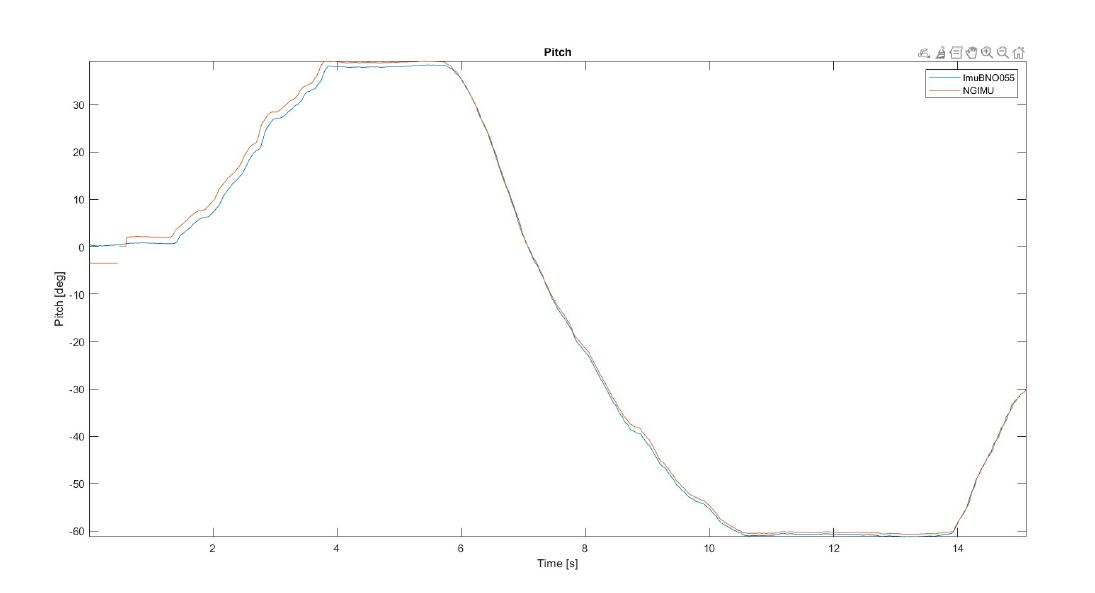
\includegraphics[width=0.8\textwidth,keepaspectratio]{figures/04_test_risultati/grafico_risultati_test.jpg}
		\caption{Esempio di grafico}
		\label{fig:grafico}
	\end{figure}
	\section{Test VL53L1X e motori}
	
	\section{Test BNO055 e servomotori}
	
	\section{Test di volo e taratura dei PID}
	
	\newpage
	\addcontentsline{toc}{chapter}{Conclusioni e sviluppi futuri}
	\section*{Conclusioni e sviluppi futuri}
	Riassumere brevemente il lavoro svolto rispetto al task assegnato, evidenziando quali risultati sono stati raggiunti e quali no. Se ci sono aspetti del task non completati spiegare quali sono stati i problemi riscontrati in merito.\\
	Inserire considerazioni personali su possibili sviluppi futuri dell'attività svolta (idee per migliorarla che non avete avuto modo di sperimentare, aspetti che suggerite di approfondire, problemi da risolvere..).
	
	\addcontentsline{toc}{chapter}{Appendici}
	\appendix
	\chapter{Appendice1}
	Se necessario ricorrete alle appendici per spiegare le parti "di contorno" dell'attività svolta e/o ciò che non riuscite ad inserire nello schema generale dei capitoli della relazione (es acquisizione dei dati con Matlab).
	
	
	\bibliographystyle{ieeetr}
	\bibliography{bibl}
\end{document}
